% !TEX TS-program = pdflatex
% !TEX encoding = UTF-8 Unicode

% This is a simple template for a LaTeX document using the "article" class.
% See "book", "report", "letter" for other types of document.

\documentclass[11pt]{cmuthesis} % use larger type; default would be 10pt
\linespread{2}

\usepackage[utf8]{inputenc} % set input encoding (not needed with XeLaTeX)
\usepackage[table,xcdraw]{xcolor}

%%% Examples of Article customizations
% These packages are optional, depending whether you want the features they provide.
% See the LaTeX Companion or other references for full information.

%%% PAGE DIMENSIONS
\usepackage{geometry} % to change the page dimensions
\geometry{a4paper} % or letterpaper (US) or a5paper or....
% \geometry{margin=2in} % for example, change the margins to 2 inches all round
% \geometry{landscape} % set up the page for landscape
%   read geometry.pdf for detailed page layout information

\usepackage{graphicx} % support the \includegraphics command and options
\usepackage{amsmath}
\usepackage{amssymb}
\usepackage{pdflscape}
%\usepackage{pdfpages}
\usepackage{tabularx}
\usepackage{bibentry}

\usepackage{algorithm2e}
%\usepackage{algorithmicx}

\usepackage[english]{babel}

% \usepackage[parfill]{parskip} % Activate to begin paragraphs with an empty line rather than an indent

%%% PACKAGES
%\usepackage{booktabs} % for much better looking tables
%\usepackage{array} % for better arrays (eg matrices) in maths
%\usepackage{paralist} % very flexible & customisable lists (eg. enumerate/itemize, etc.)
%\usepackage{verbatim} % adds environment for commenting out blocks of text & for better verbatim
%\usepackage{subfig} % make it possible to include more than one captioned figure/table in a single float
% These packages are all incorporated in the memoir class to one degree or another...





%%% END Article customizations

%%% The "real" document content comes below...

\title{Variational Methods for Energy Systems}
\author{Henning Lange}
%\date{} % Activate to display a given date or no date (if empty),
         % otherwise the current date is printed 

\begin{document}

\input{content/preconfig}
%> ------------------------------------------------------------------------------
%> This file contains most of the definitions you will need to put together
%> your thesis. All requirements were taken from the sources below:
%> http://www.cit.cmu.edu/current_students/graduates/thesis_dissertation_policies.html
%> https://www.epp.cmu.edu/graduate/thesis_format_guide.html
%> ------------------------------------------------------------------------------

%> Your title goes here.
\title{Variational Methods for Energy Systems}

%> Your own name goes here.
\author{Henning Lange}
\affiliation{Advanced Infrastructure Systems}

%> Put your previous degrees here.
\bsdegree{Cognitive Science, Universit\"at Osnabr\"uck}
\msdegree{Machine Learning \& Data Mining, Aalto University}

%> Put the month you will be graduating here, NOT the month in which you
%> actually finished the thesis. The only admissible months here are May,
%> August and December.
\Month{May}

%> Year in which you graduated (or plan to graduate).
\Year{2019}

%> Copyright notice. This may be whatever you want. My personal choice is to
%> make it as widely accessible as possible :)
\permission{\textit{Some rights reserved.} Except where indicated, this work
is licensed under a Creative Commons Attribution 3.0 United States License. 
Please see \smallurl{http://creativecommons.org/licenses/by/3.0/us/} for
details.}

%> Keywords.
\keywords{variational inference, sustainaible energy, machine learning,
non-intrusive load monitoring, alternating current optimal power flow.}
\maketitle

%> ------------------------------------------------------------------------------
%> Abstract. Mandatory and very important. Keep it under 350 words.
%> ------------------------------------------------------------------------------
\begin{abstract}
In this work, two engineering problems that could potentially lead to reductions in energy consumption and waste are identified and solutions are proposed that make use of an approximate statistical inference technique called Variational Inference. These problems encompass a sensing problem on the demand-side, namely Non-Intrusive Load Monitoring, as well as a control problem on the generation-side known as Alternating Current Optimal Power Flow. We show that the application of Variational Inference can dramatically reduce the computational time required to obtain approximate solutions to otherwise NP-hard problems by making use of an auxiliary distribution parameterized by Neural Networks that avoids any independence assumption whilst still be computationally efficient.
\end{abstract}

%> ------------------------------------------------------------------------------
%> Dedication. Optional. This is whatever you want.
%> ------------------------------------------------------------------------------
\begin{dedication}
To the one boy, with only one eye.
\end{dedication}


%> ------------------------------------------------------------------------------
%> Acknowledgements. Mandatory. At the very least you should acknowledge
%> your committee and your funding sources.
%> ------------------------------------------------------------------------------
\begin{acknowledgments}
I acknowledge my committee: Soummya Karr 
\end{acknowledgments}
\input{content/postconfig}


\chapter{Introduction}

According to the Environmental Protection Agency (EPA), in 2014, carbon dioxide ($CO_2$) made up 81\% of all green house gases emitted in the United States~\cite{EPA}. Furthermore, it is reported that ``the combustion of fossil fuels to generate electricity was the largest single source of $CO_2$ emissions in the nation, accounting for about 35 percent of total U.S. $CO_2$ emissions and 29 percent of total U.S. greenhouse gas emissions"~\cite{EPA} making electricity generation the single largest contributor to green house gas emissions overall. See Figures \ref{fig:intro} and \ref{fig:intro2} for a breakdown of $CO_2$ emissions by source and the makeup of green house gas emissions.
\begin{figure}
\centering
\includegraphics[width=0.45\linewidth]{co2b.png}
\caption[Total share of green house gas emissions by sector.]{Total share of green house gas emissions by sector~\cite{EPA}.}
\label{fig:intro}
\end{figure}

\begin{figure}
    \centering
    \includegraphics[width=0.50\linewidth]{ghgs.png}
    \caption[Make up of green house gases emitted]{Make up of green house gases emitted~\cite{EPA}.}
    \label{fig:intro2}
\end{figure}

Green house gas emissions in turn are the primary driver of climate change~\cite{change2014mitigation} and according to the EPA, climate change impacts society in many different ways. For example, climate change can influence rainfall and crop yields, affect human health, and impact forests and other ecosystems, as well as have adverse affects on the supply-side of the electrical grid."~\cite{EPA}.\\
Apart from these non-monetary costs, energy production also incurs substantial monetary expenditures: The Federal Energy Regulations Commission (FERC) estimates the total energy generation cost for the U.S. to be 112B USD annually~\cite{ferc2012history}, thus making minuscule improvements in energy efficiency often financially viable. However, considering the fact that renewable energy sources have become or are on the verge of becoming cheaper than fossil fuels~\cite{eia2016} and cost adverse consumers try to minimize energy consumption anyways, i.e. reducing energy consumption or increasing energy efficiency seems to be in everyones interest, it is pertinent to ask why sustainable energy sources have not yet found widespread adoption. The American Energy Innovation Council identifies two reasons: apart from politicism, they opine that technological advancements are required to reduce green house gas emissions associated with electricity generation and consumption~\cite{AEIC}.\\
In this work, two problems are identified and solutions are proposed whose adoption can lead to improvements to energy efficiency and energy conservation. They encompass inference and control problems on both the demand- and generation-side of the electrical grid and, as we will show later, the reason why these problems are challenging are due to computational issues, i.e. computing the exact solution to these problems is intractable because the computational cost oftentimes grows exponentially with the problem size. As we will show later, these problems share that the intractability stems from the difficulty of computing posterior distributions over binary configurations. The intractability of posterior distributions in turn usually stems from the difficulty of computing the Bayesian inversion:
\begin{align}
p(z|x) = \frac{p(x,z)}{\sum_{z' \in \mathcal{Z}} p(x,z')} \label{eq:bayes_inversion}
\end{align}
 where $z$ and $\mathcal{Z}$ denote the latent variable and its domain respectively and $x$ specifies some measured quantity. Note that for most latent domains of interest, computing the sum in the denominator (or integral when the latent variable is continuous) is computationally very hard. For the problems at hand, because the latent variable is multi-dimensional and binary, the computational complexity is in $\mathcal{O}(2^N)$ where $N$ denotes the dimensionality of the latent variable $z$. Furthermore, note that for many distributions that model temporal dependencies even computing the joint distribution can often be intractable~\cite{ghahramani1996factorial}. This intractability usually stems from the computational difficulty of computing the forward probabilities:
 \begin{align}
     p(x_t, z_t | x_{1:t-1}) = p(x_t|z_t) \sum_{z' \in \mathcal{Z}} p(z_t| z') p(z'|x_{1:t-1}) \label{eq:forward_probs_intro}
 \end{align}
 Note that similarly to (\ref{eq:bayes_inversion}), evaluating (\ref{eq:forward_probs_intro}) requires a summation over the latent domain $\mathcal{Z}$ which, again, can be computationally expensive if $\mathcal{Z}$ is large.\\
 
 When discussing these problems in more depth, we will show that current solutions make use of approximations and often-times greedy simplifying assumptions and heuristics in order to circumvent these computational costs. In this work, improvements to these approximations are sought. Specifically, we will make use of recent technological advancement in the field of Machine Learning for posterior inference that, in principle and under some conditions, allow for asymptotically exact solutions. As we will show later, we will make use of Variational Inference which circumvents the need to compute the Bayesian inversion in (\ref{eq:bayes_inversion}) by minimizing a divergence measure between the true posterior $p(z|x)$ and an approximate posterior.

\section{Problem descriptions}
We focus on two specific problems in this thesis whose solutions require obtaining an optimal binary vector, which in turn entails that $\mathcal{Z} = \{0,1\}^N$. These problems constitute Non-Intrusive Load Monitoring and Alternating Current Optimal Power Flow. The semantics of this optimal vector is different depending on the problem: In the case of Non-Intrusive Load Monitoring the optimal vector describes the most likely state of appliances in a building, whereas for Alternating Current Optimal Power Flow this optimal vector describes which generators are \emph{on} or \emph{off} in the most cost efficient configuration of generators. In the following section, brief descriptions of these problems.

\subsection{Demand-side sensing: Non-Intrusive Load Monitoring} 
Buildings account for 73\% of the energy and 40\% of the electricity consumption in the United States~\cite{li2014review}. However, knowledge about how buildings consume energy is scarce, i.e. end-users are typically faced with a monthly aggregate electricity bill. Even though, as discussed earlier, it is in the end-users interest to save energy, more fine-grained information about how much and when individual appliances consume electricity is often required to actually achieve this. According to a 2013 study~\cite{armel2013disaggregation}, providing feedback about the power consumption of individual appliances can lead to savings between 12-15\% of the energy consumed. On top of that, appliance-level energy consumption information can have secondary use-cases such as e.g. demand response~\cite{he2013incorporating}, geriatric care~\cite{alcala2015detecting}, fault detection~\cite{denucci2005diagnostic} and so on. However, obtaining this information can be costly, i.e. installing a single meter for individual appliances can be prohibitively expensive, because potential energy savings do not justify installation and maintenance costs of electricity meters for every appliance. Non-Intrusive Load Monitoring (NILM) could potentially alleviate this problem~\cite{hart1992nonintrusive}. For recent reviews of the technique, the reader is referred to ~\cite{zoha2012non,zeifman2011nonintrusive,faustine2017survey}. NILM, also called energy disaggregation, is a class of source separation algorithms whose goal it is to infer the energy consumption of individual appliances algorithmically given measurements collected at a limited number of sensing points in a building. Specifically, because power as well as current are additive, a small number of sensors is usually installed at the main distribution panel where the sum of the power draws of appliances is measured. NILM then tries to break down this sum into its summands. Arguably, one of the reasons why decades of NILM research has not produced acceptable solutions is in part due to the difficulty of the problem: Inferring the operational states of appliances is often cast as a posterior inference problem and the associated posterior distributions are usually intractable.

\subsection{Generation-side control: AC Optimal Power Flow}
Alternating current optimal power flow (ACOPF) is the scholarly term for the decades old problem of finding the optimal configuration of power generators such that demands are met throughout an alternating current transmission network, where optimality is usually defined in terms of generation cost. For a review of ACOPF and modern techniques to tackle the problem, the reader is referred to \cite{ferc2012history,capitanescu2016critical}. Note that suboptimal configurations can lead to unnecessary waste due to transmission losses and unnecessary costs due to not fully utilizing cheap generation sources. However, the potential payoff of improvements to existing solutions is big: The FERC estimates that the introduction of mixed-integer programming approaches has already saved over one-half billion dollars yearly and projects that a 5\% increase in optimality could save consumers another 6 billion dollars annually~\cite{ferc2012history}.\\
However, despite the size of potential payoffs, the FERC opines that algorithms that produce robust, fast and optimal solutions do not exist even decades after the inception of the problem~\cite{ferc2012history}. This is arguably also due to the complexity of the problem: When ACOPF is cast as a constrained optimization problem, the constraints pose computational challenges. Some of the constraints are non-linear whereas others are non-convex. As we will show later, compliance with the non-convex constraints can be achieved by turning the problem into a posterior inference problem, though, this posterior distribution is, again, intractable.



\section{Non-Intrusive Load Monitoring}

As described earlier, Non-Intrusive Load Monitoring is the problem of inferring the power consumption of individual appliances given measurements obtained at a limited number of sensing points, specifically often measurements collected at the main electrical feed of a building. The problem was first described in the seminal paper by George Hart in 1992~\cite{hart1992nonintrusive}. 

%The goal of NILM is to ultimately reduce the cost of providing appliance-level electricity measurements within a building. In the next section the potential benefits of NILM in different scenarios are discussed.
\iffalse
\section{When to use Non-Intrusive Load Monitoring?}

As mentioned earlier, the goal of NILM is to provide a service cheaper than a competing approach. In this case, the competing approach is Intrusive Load Monitoring (ILM), i.e. installing a sensor for every single appliance. Because NILM algorithms provide appliance state \emph{estimates} as opposed to real measurements, i.e. the value that NILM provides is arguably smaller compared to ILM, the question arises in which scenarios NILM is the appropriate choice for appliance load monitoring.\\
The answer to this question is dependent on numerous factors:
\begin{description}
\item[Load Monitoring application] Load monitoring in itself does provide little value without a specific intention on what to use the additional information for. Just providing the information of appliance level electricity consumption to e.g. residential customers in some cases even lead to an increase in consumption~\cite{kelly2016does}. However, there are tasks for which appliance-level consumption information is helpful such as:
\begin{itemize}
    \item Demand response: If a specific reduction in peak demand is to be achieved, appliance-level electricity consumption can facilitate the identification of appropriate actions to meet the reduction goal. For example, the knowledge that a certain relaxation of the temperature set point of an HVAC system reduces its energy consumption by a certain amount requires knowledge of the power consumption of the HVAC system.~\cite{he2013incorporating}
    \item Fault detection: Appliance faults can potentially be identified by the means of load monitoring. For example, faulty gaskets or sealings will increase the electricity consumption of fridges. Such an increase could potentially be detected by the means of load monitoring. The value of load monitoring for fault detection is a potential reduction in energy waste and improved lifetime of appliances.
    \item Operational point verification: Opposed to inferring whether or not appliances are faulty, load monitoring could also be used to verify if appliances are used correctly. Load monitoring could be used to verify if e.g. lighting are turned off at night, etc.
    \item Activity detection: Appliance usage patterns can, in principle, be used to infer information about occupants. Load monitoring could be used for occupancy detection or, going one step further, to infer 'Activities of Daily Living' (ADL). Inferring ADLs in a cost effective way could be helpful in e.g. geriatric care and reduce the need for either additional sensing equipment or other intrusive or costly methods to infer ADLs such as interviews.~\cite{alcala2015detecting}
\end{itemize}
\item[Appliances types] Whether or not a NILM approach will be successful crucially depends on which appliances are to be monitored. NILM as opposed to ILM solutions will oftentimes struggle with appliances that have highly varying signatures and appliances that consume little power. There are numerous appliances that NILM algorithms struggle with such as personal computers, printers, phone chargers, etc. However, for other appliances a NILM solution might yield appliance state estimates that are sufficient for the load monitoring application at hand such as appliances with regular signatures like e.g. traditional fridges and appliances with a high power draw such as kettles. Note that when multiple appliances of the same make and model are present within the aggregate, NILM algorithms will most likely fail to distinguish them. Because their features will most likely be close to identical, most NILM algorithms will lump these appliances together which in turn means that the value that NILM solutions provide is limited in such a scenario.
\item[Number of appliances of interest] If the specific load monitoring application only requires appliance energy estimates for very few appliances, there is little to gain from a NILM solution. However, when a more holistic energy monitoring approach is to be employed, i.e. when multiple load monitoring applications are to be tackled in parallel and the number of appliances for which load estimates are required is high, the potential savings by making use of NILM are high.
\item[Potential value] If the value of the load monitoring application is below a certain threshold, there is no incentive to either use an ILM or NILM solution. On the flip side, if the potential value of the load monitoring solution is above a certain threshold, it is hard to justify a non-intrusive solution. The additional cost of installing more meters outweigh the uncertainty that is inherent to a non-intrusive solution. NILM solutions will be the most economical approach to load monitoring between these two thresholds, i.e. when the potential value of the load monitoring application is large enough to warrant the installation of at least one meter and when potential value is small enough such that ILM is not economical.
\end{description}
\fi



\subsection{State of current research}

\subsubsection{Event-Based approaches}
\begin{figure}
\centering
\includegraphics[width=0.8\linewidth]{nilm_hart.png}
\caption[A graphical depiction of the NILM process.]{A graphical depiction of the NILM process taken from the seminal paper by Hart 1992. Taken from~\cite{hart1992nonintrusive}}
\label{fig:hart}
\end{figure}

\begin{figure}
    \centering
    \includegraphics[width=0.65\linewidth]{nilm_event.png}
    \caption[Schematic of the data flow of generic event-based NILM algorithms.]{Schematic of the data flow of generic event-based NILM algorithms. Taken from~\cite{anderson2012event}.}
    \label{fig:hart2}
\end{figure}


 Figures \ref{fig:hart} and \ref{fig:hart2} show graphically how early approaches operated, i.e. they tackled the problem by detecting sudden changes~\cite{anderson2012event}, so called events, in the aggregate power followed by a feature extraction phase~\cite{patri2014extracting}, i.e. signatures of the detected events are extracted in the hopes that classification algorithms can associate appliances with the extracted event features~\cite{pereira2015semi}. After a sequence of labeled events is extracted, this discrete time series is then in turn transformed into a power trace for each appliance.\\
Even though this approach was refined in numerous ways by e.g. using transient and high frequency information as features for classification~\cite{norford1996non}, improving the energy estimation phase~\cite{giri2015energy} or post processing of the extracted event sequence~\cite{he2016non}, generalizable and accurate power estimates could not be achieved. One of the reason why these event-based approaches struggle is the fact that the individual algorithmic stages make independent and local decisions which leads to errors propagating through the different algorithmic steps, i.e. the classification stage could result in a nonsensical sequence of appliance switches, i.e. it could e.g. result in a sequence where an appliance is assumed of having turned \emph{off} at time point $t$ even though it already was assumed to be \emph{off} at time point $t-1$. The energy estimation stage of the algorithmic chain is then tasked to achieve something impossible, i.e. transform a nonsensical event sequence into power estimates of individual appliances.
\subsubsection{Temporal Motif Mining}
One approach to overcome the problem of errors propagating through the stages of event-based approaches is Temporal Motif Mining (TMM)~\cite{shao2012temporal}. Specifically, the approach tries to tackle potentially nonsensical event sequences. TMM in a sense, merges the classification and energy estimation phase, i.e. it tries to solve both problems jointly, specifically, by trying to match events such that 
\begin{enumerate}
\item The sum of power changes of an event sequence is nearly 0.
\item Every prefix sum of event sequences is positive.
\item Power changes cannot be smaller than a certain percentage of the biggest transition in an episode.
\end{enumerate}
However, since the learning objective of TMM is combinatorial, simplifying assumptions over possible event sequences were made, such that no more than $x$ events can lie between events from the same appliance. Even though these approaches avoided the problem of nonsensical event sequences successfully, the assumption that an appliance episode is zerosum is often overly simple because appliances often exhibit transient behaviors and furthermore, the approach suffers from the reliance on a perfect event detector, i.e. if an event was missed, TMM struggles. Thus, even though the problem of error propagation from the classification into the energy estimation phase is mitigated by TMM, errors can still flow from the event detection into the energy classification stage.

\subsubsection{State-based approaches}
In order to overcome the problem of error propagation through the algorithmic stages, ideally, energy disaggregation is performed in an end-to-end manner, i.e. by a single unified model that tells the generative story of the aggregate power measured at the main distribution. Because the states of several appliances evolve independently in parallel and the aggregate observation is a function of all hidden states, Factorial Hidden Markov Models lend themselves as a modeling choice~\cite{ghahramani1996factorial}. Factorial Hidden Markov Models are a generalization of Hidden Markov Models where multiple hidden chains evolve marginally independent and the aggregate observation $x_t \in \mathbb{R}^S$ at time point $t$, is a function of all hidden states $z_t \in \{0,1, ..., K\}^N$, with $S$ being the observation dimensionality, $K$ being the number of states each hidden chain can take and $N$ being the number of latent chains. See Figure \ref{fig:fhmm} for a representation of the associated graphical model. The joint distribution is defined as the following:
\begin{align}
p(x_{1:T},z_{1:T}) = \prod_t^T p(x_t|z_t)\prod_i^N p(z_{t,i}|z_{t-1,i})p(z_{0,i})
\end{align}

\begin{figure}
\centering
\includegraphics[width=0.5\linewidth]{FHMM.png}
\caption[The graphical model corresponding to Factorial Hidden Markov Models.]{The graphical model corresponding to Factorial Hidden Markov Models. Multiple hidden chains evolve independently in parallel whereas the observation at time point $t$, $x_t$ is a function of all hidden. Graphic taken from~\cite{parson2012non}}
\label{fig:fhmm}
\end{figure}

Each appliance is then modeled by a single HMM chain and the aggregate observation constitute the measurements collected at the main electrical feed of the building. Supervised energy disaggregation can then be posed as inference in the associated probabilistic model, i.e. inferring $z^* = \arg\max_z p(z_{1:T}|x_{1:T})$, whereas unsupervised energy disaggregation can be posed as the learning problem. Note that inference is computationally intractable mainly because of the fact that the individual latent chains become dependent conditioned on the observation and fact that the number of possible states grows exponentially with the number of hidden chains. This also entails that unsupervised energy disaggregation is computationally intractable, because inference is usually required for learning.

\begin{description}
\item[Iterative Viterbi] The problem of computational intractability of learning and inference in FHMMs has been tackled in a number of ways. In~\cite{parson2012non}, the problem is tackled by iteratively applying the Viterbi algorithm to a single latent chain. Specifically, parameterized general models of appliance types were specified and then iteratively, the parameters were fit to the observation and the Viterbi algorithm was used to compute the most likely state sequence for an appliance type. Then, this appliances contribution to the aggregate was removed and the process was repeated. Even though, this procedure allows for inference as well as limited learning, it is not invariant to the order in which appliances are processed, i.e. processing appliances in different orders will lead to different results.
\item[Optimization] In comparison, the AFAMAP algorithm poses inference as an optimization, specifically an integer programming problem~\cite{kolter2012approximate,shaloudegi2016sdp}. Specifically, by introducing the one-at-a-time constraint postulating that only a single HMM chain can change states at any given point in time, posterior inference is converted into a convex quadratic programming problem by relaxing the integer constraints associated with the integer program that results from translating posterior inference into such a problem. Additionally, a robust mixture model is introduced that absorbs power associated with appliances for which no ground truth is provided and the difference signal is modeled to improve accuracy. Even though the inference engine seems powerful and could in principle be extended to perform exact inference of the mode of the posterior by e.g. employing branch-and-bound, this approach has drawbacks. The inference technique needs to be provided with ground truth and will only produce power estimates for appliances for which ground truth is provided. In the paper, the authors describe an unsupervised strategy for obtaining ground truth, however this approach seems to not generalize well to other datasets. On top of that, extending the algorithm to handle the learning problem is challenging since solving the convex quadratic program only yields the mode of the distribution, therefore making the application of EM-like algorithms difficult. Only hard-EM schemes like Viterbi learning could in principle be employed though they often underfit considerably~\cite{gutmann2008parameter}. Furthermore, a na\"ive implementation of such an EM-scheme would only improve the model parameters for the appliances for which ground truth estimates are available. Moreover, strategies that try to extract ground truth for all appliances by iteratively subtracting appliance power traces for which estimates are available struggle with subtraction artifacts, i.e. because appliance estimates are imperfect, subtraction will effectively result in the addition of residuals that depending on the amplitude can easily confuse the ground-truth extraction module of the algorithm.
\item[Markov Chain Monte Carlo] On the other hand, Markov Chain Monte Carlo (MCMC) techniques were employed in order to deal with the intractable posterior distributions of the FHMM distribution~\cite{johnson2013bayesian,jia2015fully,el2009rjmcmc,egarter2015paldi}. In~\cite{johnson2013bayesian}, Factorial Hidden Markov Models were additionally extended to handle semi-Markovian state transitions trying to overcome the implicit assumption introduced by the Markov property of Hidden Markov Models, namely that the distribution of state durations, i.e. the time each Markov chain spends in a single state, is geometric. In the context of energy disaggregation, assuming geometrically distributed state durations is usually not valid.\\
The general idea of MCMC algorithms is to construct a Markov Chain whose equilibrium distribution provides a sample of the intractable posterior distribution. It can be shown that Gibbs sampling~\cite{casella1992explaining}, i.e. repetitively sampling from the conditional posterior distribution, constitutes a Markov Chain whose equilibrium distribution can provide a sample from the posterior distribution and that the quality of the sample improves with the length of the Markov Chain~\cite{geman1987stochastic}. However, Gibbs-based MCMC techniques in the context of energy disaggregation have two drawbacks. First, because posterior distributions in the context of energy disaggregation exhibit strong multi-modality, Gibbs samplers often exhibit very slow mixing of the posterior and therefore require prohibitively long Markov chains in order to acquire a high-quality sample of the posterior. The multi-modality of the posterior distribution encountered in the context of energy disaggregation can be explained by the fact that multiple appliances often exhibit a similar power draw, thus more than one appliance might be able to explain away the aggregate consumption. For illustration, consider a scenario with 2 two-state appliances with comparable power draw and an aggregate observation $x'$ that is similar to the power consumption of each appliances. Thus we can assume that for the posterior the following holds:
\begin{align*}
p(z|x') &= \begin{pmatrix}
0&
0.5&
0.5&
0
\end{pmatrix}\\
 \text{with } z &=\begin{pmatrix} 0,0&
0,1 &
1,0 &
1,1 
\end{pmatrix}
\end{align*}

A Gibbs sampler that resamples a single latent variable will `get stuck' in either of the modes ($z = (0,1)$ or $z = (1,0)$), i.e. in this contrived example the modes constitute probability islands which the sampler will never escape. In more realistic scenarios, when all probabilities are strictly greater than 0, even though the sampler will escape modes eventually, this process can be prohibitively slow. Second, even though these approaches allow for learning by introducing distributions over model parameters, inference is computationally expensive. Because of the multi-modality of the posterior that causes slow mixing, for every data point, an often times quite long Markov chain needs to be computed. Ideally inference takes a functional form that incurs little computational costs.
\iffalse
\item[Variational Inference] As stated earlier, recent advances in Bayesian optimization, specifically, Variational Inference and in particular the introduction of recognition distributions have led to the development of methods that allow for amortized statistical inference. 
Amortizing VI has been employed to the problem of energy disaggregation~\cite{ng2016scaling}, however even though temporal dependencies were modeled by making use of Gaussian copulas, because feed forward neural networks were used to parameterize the auxiliary distribution $Q$, temporal dependencies could not be modeled at the edges of temporal minibatches. Another drawback of the approach is the choice of objective function in conjunction with the choice of the auxiliary distribution: as an objective the ELBO introduced in \eqref{eq:ELBO} was used. As stated earlier, implicitly, the ELBO objective minimizes the backward KL-divergence. It can be shown that minimizing the backward KL-divergence is zero-forcing, i.e. most probability mass in $Q$ will be assigned to the mode of $P$. Because as an auxiliary distribution a factored multi-variate Bernoulli distribution is chosen, i.e.
\begin{align*}
 q_\sigma(z) = \prod_i^N \sigma_i^{z_i}(1-\sigma_i)^{1-z_i}
\end{align*}
with $\sigma \in [0,1]^N$ being the vector of coin-flip probabilities, it can be shown that:
\begin{align*}
 \arg \min_{\sigma} D_{KL}(Q_\sigma||P) &= \arg \min_{\sigma} \sum_{z \in \mathcal{Z}} q_\sigma(z)\log \frac{q_\sigma(z)}{p(z)} = \arg \max_z p(z|x)
\end{align*}
Thus, minimizing the backward KL-divergence will lead to $Q$ learning the mode of $P$ which in turn entails that the resulting learning algorithm will assign most probability mass to a single latent configuration $z$. In the experience of the author, this is problematic in the context of energy disaggregation and leads to considerable underfitting. This is because, ideally, when a change in aggregate power suggest that an appliance has changed its state, the uncertainty of previous state changes should be taken into consideration. For example, consider a scenario where the algorithm is unsure whether an \emph{off}-transition should be associated with appliance $a$ or $b$ and future observations strongly indicate an \emph{on}-transition for appliance $a$, then the algorithm should assign more probability mass to the state sequence in which appliance $a$ turns \emph{off} in the past.
\fi
\item[Function Learning] Recently, approaches emerged that directly try to learn a function that maps aggregate observations to single appliance power traces or energy estimates~\cite{kelly2015neural}. These approaches usually assume knowledge of single appliance episodes and training is facilitated by creating synthetic aggregate observations by randomly summing up these episodes. Function approximators are then trained to infer the power or energy consumption of single appliances. These approaches make the implicit assumption that patterns introduced by other appliances when inferring the power consumption of one appliance can be considered noise and will be ignored by the function approximator. However, that assumption is in the opinion of the author not valid because the patterns introduced by other appliances are highly structured and will often confuse function approximators. Furthermore, apart from being inherently supervised, these approaches struggle with shifts in the data distribution, thus making even a simple shift in the baseload potentially a problem for these approaches. However, these approaches might find application in niche scenarios where the load composition is known and static. For other approaches based on this idea, see \cite{zhang2018sequence,barsim2018neural,salerno2018extreme,de2018appliance,roos1994using}
\end{description}

\subsection{Knowledge Gaps}

For state-based NILM algorithms, one of the biggest challenges seems to be the computational burden associated with the learning problem in graphical models appropriate for NILM. This problem seems to not have been solved sufficiently: some algorithms circumvent learning altogether by applying heuristics to acquire ground truth, other algorithms avoid the combinatorial nature of the problem by performing learning one-appliance-at-a-time whereas other approaches rely on computationally expensive and typically slow approaches for learning. Thus, existing algorithm either introduce considerable bias or are too expensive for real-world applications. Note that because exactly solving the learning problem is known to be a NP-hard problem, any successful algorithm performs some kind of approximation. Ideally, such an approximate algorithm is (asymptotically) unbiased and incorporates a parameter that allows to trade-off computational time for accuracy. An approximate but asymptotically unbiased algorithm that allows trading computational burden for accuracy is still missing.\\
Furthermore, so far, even though many publicly available data sets contain high frequency information, most algorithms typically only make use of information at a much lower sampling frequencies. Although event-based algorithms sometimes employ features extracted from high frequency measurements, for state-based algorithms, high sampling rates are oftentimes solely used to compute accurate active and reactive power measurements. Thus, state-based algorithms, so far, discard a potentially vital source of information and the question arises whether high frequency information can be used to improve state-based energy disaggregation algorithms.

\newpage
\subsection{Research Questions}
\subsubsection{Research Question 1.1}

Because state-based algorithms do not make sufficient use of high frequency information, the following research questions arise:

\begin{enumerate}
\item How can we leverage high frequency information from voltage and current measurements in a computationally efficient manner to obtain appliance state estimates?
\item What is the performance of the resulting algorithm in terms of disaggregation error in an unsupervised and supervised setting?
\end{enumerate}

The publication in section \ref{chapter:bolt} answers these research questions. The resulting paper was published in the \emph{Proceedings of the 3rd ACM International Conference on Systems for Energy-Efficient Built Environments}.

\newpage
\subsubsection{Research Question 1.2}
The algorithm resulting from answering research question 1.1 has shown promising results. However, it has some fundamental drawbacks. Because only micro-temporal dependencies are exploited, i.e. temporal dependencies within a single voltage-cycle, some degree of supervision is required to achieve acceptable disaggregation results. However, for a NILM algorithm to be commercially viable, disaggregating energy in an unsupervised fashion is paramount. When introducing temporal dependencies into the model, a computationally efficient strategy to approximate the forward probabilities defined in (\ref{eq:forward_probs_intro}) is required. Because of this, the following research questions arise:

\begin{enumerate}
\item How can a computationally efficient approximation of the filtering recursion be obtained that allows for temporal regularization?
\item What is the performance of the resulting algorithm in an unsupervised setting?
\end{enumerate}

The publication in section \ref{chapter:varbolt} answers the research questions above. The resulting paper was published in the \emph{Proceedings of the 2018 AAAI Conference on Artificial Intelligence}.

\newpage
\subsubsection{Research Question 1.3}

The algorithm introduced by answering Research Question 1.2 makes use of a factored multi-variate Bernoulli distribution. In order to avoid a parameterization that grows exponentially with the number of appliances, this distribution makes an unnecessary independence assumption, specifically, that states of appliances are independent given previous observations. As will be shown later, this independence assumption makes it difficult to learn either-or relationships. Because of this, the following question arises:

\begin{enumerate}
\item How can a distribution as flexible as a mutli-variate Bernoulli be parameterized such that the parameterization does not grow exponentially?
\end{enumerate}

This research question is answered in the publication in section \ref{chapter:factornet}. It was published in the \emph{Proceedings of the 4th International Workshop on Non-Intrusive Load Monitoring. 2018}.

\newpage
\subsubsection{Research Question 1.4}

The time-complexity of the algorithm introduced by answering Research Question 1.2 was mainly reduced by making an application-specific sparsity assumption as well as exploiting the structure of a factorized posterior distribution in conjunction with the factorization inherent to FHMMs. However, as stated earlier, using this factored posterior limits the accuracy of the inference technique and, on top of that, despite of the sparsity assumption, the scalability of the algorithm is limited. The question arises whether we can abolish these simplifying assumptions that were required to ensure computational efficiency but still be computational efficient. Note that because such an approach does not exploit structure unique to NILM, i.e. it is a generic algorithm for inference and learning in dynamical systems, the following question arises:

\begin{enumerate}
\item What is an asymptotically unbiased algorithm for inference in learning in non-linear stochastic dynamical systems with binary latent states?
\item How sample-efficient is the resulting algorithm?
\end{enumerate}

The publication in section \ref{chapter:nvif} answer this research question. It was published in the \emph{Proceedings of the 2019 International Conference on Acoustics, Speech, and Signal Processing}.

\newpage
\section{Problem Statement: AC Optimal Power Flow}


As stated earlier Alternating Current Optimal Power Flow (ACOPF) tries to answer the question of how to configure generators in an alternating current transmission network optimally such that generation meets demand. Generation meets demand when a set of non-linear constraints, the so called power flow equations, are satisfied. Optimality is defined by minimizing an objective function. ACOPF should not be confused with two similar and related problems, i.e. the load flow problem and economic dispatch. The former problem deals with inferring the system state given partial knowledge, i.e. solving the power flow equations, whereas the latter is concerned with optimally dispatching power whilst ensuring a power reserve but by simplifying or completely ignoring the power flow equations.

\subsection{State of current research}

Early approaches to optimally operate alternating current transmission networks relied on ``experienced engineers and operators using judgment, rules of thumb, and primitive tools"~\cite{cain2012history}. However, soon computational tools were introduced. In as early as 1929, analog network analyzers that model the transmission network were used to solve the power flow equations\cite{cain2012history}. Then, in 1956, Ward and Hale introduced the first automated and digital power flow solver~\cite{hale1956digital}. In 1962, Carpentier introduced the optimality conditions for the ACOPF problem based on Karush-Kuhn-Tucker conditions which is considered today to be the first formulation of the ACOPF problem~\cite{carpentier1962contribution}. Even though there are many different ACOPF formulations with different objectives, most ACOPF formulations can be represented by the following standard form:
\begin{align*}
min_x f(x)\\
\text{s.t. } g(x) &= 0\\
h(x) &\leq 0
\end{align*}
where $f$ is the objective function to minimize, usually the generation cost, and $h$ and $g$ are constraint functions that describe the power flow equations, system constraints and control limits. As stated earlier, in order to ensure that the system is in a physical state and that generation meets demand considering the transmission losses, the power flow equations need to be satisfied. There are multiple equivalent formulations of the power flow equations. However, the most commonly used are in polar form~\cite{schaffer1988nondiverging}:
\begin{align*}
0&=-P_{{i}}+\sum _{{k=1}}^{N}|V_{i}||V_{k}|(G_{{ik}}\cos \theta _{{ik}}+B_{{ik}}\sin \theta _{{ik}}) = g_i\\
0&=-Q_{{i}}+\sum _{{k=1}}^{N}|V_{i}||V_{k}|(G_{{ik}}\sin \theta _{{ik}}-B_{{ik}}\cos \theta _{{ik}}) = g_{i+N}
\end{align*}
Thus, the power flow equations describe the non-linear relationship between nodal voltages $V_i$ and active and reactive power ($P_i$ and $Q_i$) in the transmission network specified by the admittance matrix $Y_{ik} = G_{ik} + jB_{ik}$. Note that $N$ specifies the number of buses and $\theta _{{ik}}$ the difference in voltage angle between bus $i$ and $k$. Although equivalent, the power flow equations can also be expressed in matrix form with $S_i = P_i + jQ_i$, $S \in \mathbb{C}^N$, $V \in \mathbb{C}^N$ and $Y \in \mathbb{C}^{N \times N}$,
\begin{align*}
0 = S - diag(V)(YV)^* = g
\end{align*}

Note that in many instantiations of the ACOPF problem, the inequality constraints specify control limits of the nodal voltages and active and reactive power generation. Note that power generation constraints are often non-convex, i.e.
\begin{align*}
h_i = P_i - P^{max}_i o_i \leq 0\\
h_i =  P^{min}_i o_i - P_i \leq 0
\end{align*}
with $o_i \in \{0,1\}$ specifying whether a generator is online.\\
Even though the cost function $f$ is often well-behaved and e.g. convex, constraints are usually non-convex and non-linear.\\

Because the non-convexities encountered in the ACOPF constraint set can usually be represented by integer constraints, mixed integer program solvers based on e.g. branch-and-bound~\cite{lawler1966branch} can be employed to deal with the non-convexities. However, because multiple, and in the worst case exponentially-many, linearly relaxed problems need to be solved, these approaches incur substantial computational cost and require a \textbf{robust}\footnote{Robust in this context means that convergence to the physical solution can be guaranteed.} solver for the relaxed sub-problems.\\

Furthermore, the non-linearities encountered in the ACOPF problem pose additional challenges. Because of their non-linear nature, the power flow constraints do not exclude all non-physical solutions. It can be shown that for the much simpler load flow problem, a transmission system consisting of $N$ buses can have up to $2^N$ solutions even though there is only one single physical solution~\cite{thorp1997load,tamura1983relationship}. This entails that the load flow problem is underspecified, i.e. the power flow equations are solely a necessary condition for a solution to be physical but they are not sufficient.

\subsubsection{Decoupled-OPF}
In order to overcome the problem of under-specificity of the ACOPF formulation, approaches were developed that linearize the power flow equations~\cite{stott1974fast}. Specifically, by making two assumptions a bilinear approximation of the power flow equations can be obtained.
\begin{enumerate}
\item The imaginative part of the admittance matrix dominates the real part, thus assuming that $Y_{ik} = jB_{ik}$ is a valid approximation
\item Because voltage angles are small, $\cos(\theta_{ik}) \approx 1$ and $\sin(\theta_{ik}) \approx \theta_{ik}$
\end{enumerate}
which results in the equations:
\begin{align*}
0 = P_i - \sum_{k=1}^N |V_i||V_k| B_{ik} \theta_{ik} = g_i\\
0 = Q_i - \sum_{k=1}^N -|V_i||V_k| B_{ik} \theta_{ik} = g_{i+N}
\end{align*}
If furthermore it is assumed that voltage magnitudes are approximately unit, the power flow equations can be reduced to:
\begin{align*}
0 = P_i - \sum_{k=1}^N B_{ik} \theta_{ik} = g_i
\end{align*}
 Note that if the constraints are linear, introducing these simplifying assumptions results in a linear program that can be solved efficiently by e.g. the Simplex algorithm or Interior Point methods~\cite{klee1970good}.\\
Even though this formulation effectively disregards all network transmission losses, it is used in many commercial and industrial applications as a de facto standard but according to~\cite{stott2009dc}, the formulation introduces unacceptable errors in large systems.

\subsubsection{Full ACOPF solvers}
To avoid these errors for large systems, many different ACOPF solvers that operate directly on the non-linear power flow equations were proposed.

\begin{description}
\item[Sequential Linear Programming] One such algorithm to solve the ACOPF problem is Sequential Linear Programming (SLP)~\cite{kirschen1988mw}. SLP tries to solve non-linear programs by a series of linear approximations, i.e. SLP is an iterative procedure that solves a linear program at every iteration. Specifically, given a guess about the solution $x_0$, a linear program (LP) relaxation around $x_0$ is performed and the resulting LP is solved by an LP solver, typically either by variants of the Simplex Method or an Interior Point solver, in order to obtain a better guess $x_{i+1}$. The linear program relaxation is obtained by a first order Taylor series expansion and every iteration is proved to improve the objective, therefore guaranteed to find a local optimum.
\item[Sequential Quadratic Programming] Similarly to SLP, Sequential Quadratic Programming (SQP) is an iterative process that solves an optimization problem at every iteration~\cite{grudinin1998reactive}. However, instead of performing a first order Taylor expansion, a second order expansion is performed resulting in a quadratic program to solve at every iteration. Because second order information are leveraged, SQP usually converges faster than SLP. Note that when the program is unconstrained, SQL will reduce to performing Newton-Raphson.\\

These approaches implicitly assume that applicable functions display “suitable convexity”~\cite{carpentier1962contribution}, i.e. implicitly it is assumed that gradient-based approaches will find physical solutions despite the non-convexity of e.g. the power flow constraints. This becomes abundantly clear when realizing that all of the introduced solvers rely on an initial guess of the optimal solution $x_0$, also called the seed or initial point, and follow some kind of gradient that results from either solving an LP or QP or some program involving barrier or penalty functions. Ultimately, these solvers perform projected gradient steps. The authors of~\cite{hiskens2001exploring,schecter2013exploration} argue that given the structure of the power flow equations, the assumption of ``suitable convexity" may be a big assumption.\\

The fact that ``suitable convexity" might be an invalid assumption is further supported by research that investigates the convergence properties of solvers for the power flow equations. It can be shown that Newton-Raphson based solvers exhibit a property commonly referred to as \emph{Newton fractals}~\cite{klump2000new,thorp1997load}, i.e. convergence to the true solution can only be guaranteed if the seed point $x_0$ is ``close enough" to the true solution because ``the boundaries between basins of attraction under the iterative scheme are fractal. As two or more solutions get closer, their basins become more and more intertwined, so that, the neighborhood of any given solution becomes peppered by points attracted to different ones"~\cite{trias2012holomorphic}. Figure \ref{fig:fractals} shows an example of \emph{Newton fractals} graphically.\\

\begin{figure}
\includegraphics[width=\linewidth]{fractals.png}
\caption[Fractal basins of attraction for the two-bus load flow problem, under
the FDLF (Decoupled-PF) method.]{``Fractal basins of attraction for the two-bus load flow problem, under
the FDLF (Decoupled-PF) method. Initial seeds that lead to the correct solution are shown in
green; to the spurious solution in red; and non-convergence in black."~\cite{trias2012holomorphic}}
\label{fig:fractals}
\end{figure}

Because of \emph{Newton fractals}, these approaches are in danger of not finding any physical solution at all because as described earlier and shown in Figure \ref{fig:fractals}, the power flow equations have solutions which are not physical, i.e. there are assignments to the complex nodal voltages and complex power such that the power flow equations are fulfilled that can however not be realized physically. These spurious solutions act as attractors, i.e. the power flow solvers introduced earlier, because solutions are obtained by projected gradient steps, might be attracted to these false solutions, in order to reach their goal of satisfying the power flow equations.\\

Note that because these solvers are deterministic, the solution depends crucially on the guess of the initial solution $x_0$. That is why researchers have tried to alleviate these convergence issues by initializing $x_0$ in a way that encourages convergence to the true solution, i.e. by initializing $x_0$ with the solution to a simpler problem such as the solution to decoupled-OPF~\cite{leonidopoulos1995approximate,klump2000techniques,stott1971effective}.\\
\item[Continuation] Another strategy is to the employ the continuation method, in the context of ACOPF also called power stepping, by iteratively solving problems by scaling demand by a factor $\lambda$ and use the solution obtained for small $\lambda$ as the initial guess for a solution at a bigger $\lambda$ starting at $\lambda = 0$ until the original problem is recovered at $\lambda = 1$~\cite{milano2009continuous}. Especially for problems whose solution is close to the feasibility boundary where convergence issues are predominant, it is easier to obtain solutions further away from the feasibility boundary and then follow the solution paths to $\lambda = 1$. 
\item[Homotopy] A similar strategy is the Homotopy method whose general idea is the following: similarly to the continuation method a scaling factor $\lambda$ is introduced, however for the Homotopy method, $\lambda$ interpolates between two functions~\cite{okumura1991solution,ponrajah1989minimum}. Specifically, if one tries to infer complex voltages $v$, the Homotopic function $H$ can be defined as:
\begin{align*}
H(v,\lambda) = \lambda g(v) + (1-\lambda) \hat{g}(v)
\end{align*}
In this case $\hat{g}$ is some function and $g$ denotes the power flow equations. Varying $\lambda$ and following the solution path can allow for finding solutions for ill-conditioned problems, i.e. for problems that do not converge when the initial guess is a flat (all load voltage
magnitudes equal to 1 and all bus voltage angles equal to
0).\\

However, both the Continuation and Homotopy methods incur substantial computational cost because numerous ACOPF problems need to be solved for varying $\lambda$. Note that these costs multiply when integer constraints are handled by branch-and-bound algorithms. For every branch, a relaxed optimization problem needs to be solved and if this relaxed problem is in turn solved by the Continuation and Homotopy method which requires solving multiple problems for varying $\lambda$, the number of requires solutions oftentimes explodes.
\item[Holomorphic Embedded Load Flow Method] In the context of the load flow problem, these issues were recently addressed by the introduction of a solver called Holomorphic Embedded Load Flow Method (HELM) \cite{trias2012holomorphic,trias2015fundamentals}. Specifically, HELM overcomes the problem of multiple solutions by performing analytic continuation of a function at a solution known to be physical~\cite{beach2000reliable}. Note that analytic continuation yields a unique solution if the function to continue is holomorphic~\cite{range2013holomorphic}. Which solution is found depends on the point from which continuation is performed and the authors of HELM argue that holomorphic continuation from a known physical solution ``guarantees that the solution always corresponds to the correct operative solution, when it exists; and it signals the non-existence of the solution when the conditions are such that there is no solution"~\cite{trias2012holomorphic}. However, so far, HELM has only found applications in the realm of power flow as opposed to \emph{optimal} power flow.
\end{description}

\subsection{Knowledge Gaps}

As described earlier, because of the non-linearity of the power flow equations, existing optimal power flow solvers lack robustness because convergence to non-physical solutions that nevertheless satisfy the power flow equations cannot be ruled out. Furthermore, because of non-convex in particular integer constraints, these approaches incur substantial computational cost. To put it into the words of the FERC, ``even 50 years after the problem was first formulated, we still lack a \textbf{fast} and \textbf{robust} solution technique for the full ACOPF problem"~\cite{cain2012history}.\\
Furthermore, as stated earlier, HELM overcomes some of the convergence issues of traditional load flow solvers by embedding the power flow equations into holomorphic functions. Even though this strategy seems to alleviate the problem of the ambiguity of the power flow equations, there is no straight-forward way for HELM to be used in \emph{optimal} power flow applications.

\newpage
\subsection{Research Questions}
Existing approaches for ACOPF seem to predominately be based on optimization strategies and the question arises whether a learning-based approach can overcome some of the problems introduced earlier. Specifically, can a function be learned that produces optimal and feasible generator configurations given demand assignments reliably and fast? Note that because ACOPF solutions need to comply with numerous safety constraints, it is paramount that this function produces outputs that comply with these constraints. Furthermore note that, because generators can be shutdown completely, the action-space of such a learning based approach is non-convex. The following questions arise:

\begin{enumerate}
    \item How can the ACOPF problem be formulated as a learning problem?
    \item Given a learning-based formulation:
     \begin{itemize}
        \item How can a learning signal be obtained?
        %\item What is a load flow solver that allows for differentiation through its operators?
        \item How can safety constraints like e.g. voltage magnitude constraints be enforced?
        \item What is a computationally efficient strategy to deal with non-convex action spaces?
    \end{itemize}
\end{enumerate}



\chapter{Variational Inference}
Successful solutions to the problems discussed above have one thing in common: they allow to obtain an optimal binary vector. This process can be posed as statistical posterior inference in distributions over binary configurations. However, because the normalizing constant of these distributions usually involves enumerating all binary states, posterior inference is oftentimes computationally intractable because the number of possible binary configurations grows exponentially with the dimensionality of this vector, therefore requiring approximate inference techniques. For example, in the case of ACOPF, every generator is associated with a binary variable and even moderately sized problems can have up to 50 generators. Thus, na\"ive inference on posterior distribution of that size would require evaluating $2^{50} \approx 10^{15}$ generator configurations.\\
There seem to be a dichotomy in approximate approaches to deal with intractable posterior distributions. On one hand, there are Markov Chain Monte Carlo techniques which are a collection of tools to draw samples from the desired posterior. Specifically, a Markov chain is introduced whose equilibrium distribution converges to a sample from the posterior~\cite{geman1987stochastic}. It is well known that the quality of the sample increases with the length of the Markov Chain, however, this process is often too slow when the probability surface is multi-modal, i.e. the Markov Chain can `get stuck' in modes of the posterior which leads to prohibitively slow mixing~\cite{geyer1992practical}. 

On the other hand, Variational Inference~\cite{wainwright2008graphical} techniques have emerged as an alternative tool to deal with intractable posterior distributions. Variational Inference turns stastistical inference into an optimization problem by optimizing parameters of an auxiliary distribution $Q$ such that $Q$ best approximates $P$. Because the true posterior is approximated by an auxiliary distribution, unless $Q=P$, VI is an approximate inference technique, whereas MCMC is asymptotically exact albeit being slow. Recent advances have greatly improved the scalability, applicability, speed and accuracy of VI based approaches. Because of these advances, especially in terms of speed, modern VI approaches seem to be a prime candidate to control and observe physical systems in real time.

In this section a brief overview on Variational Inference is provided. For a more thorough discussion of VI the reader is refered to~\cite{blei2017variational,zhang2017advances}. The main idea behind VI is the following: Given a distribution $P$ for which posterior inference is intractable, posterior inference is translated into an optimization problem. Specifically, a tractable distribution $Q_\psi$ parameterized by the variational parameters $\psi$ is introduced and the parameters $\psi$ are optimized in such a way that $Q_\psi$ best approximates $P$ as measured by some divergence criterion. Then, in order to perform inference on $P$, because $Q_\psi$ is maximally similar to $P$ but tractable, inference is performed on $Q_\psi$ instead.\\
Because acquiring samples from or computing $p(z|x)$ is intractable, directly minimizing $D(q(z|x)||p(z|x))$ with $D$ being some divergence measure is usually intractable. In order to overcome this problem, a surrogate loss is minimized. By making use of Jensen's inequality~\cite{kuczma2009introduction}, it can be shown that:
\begin{align}
\log p(x) &= \sum_z \log p(x|z) p(z)\\
              &= \sum_z \frac{q(z|x)}{q(z|x)} \log p(x|z) p(z)\\
              &\geq D_{KL} [q(z|x) || p(z)] + \mathbb{E}_{q(z|x)} [\log p(x|z)]\label{eq:ELBO}\\
              & = \log p(x) - D_{KL}(q(z|x) || p(z|x)) \label{eq:lowerbound}
\end{align}
with $D_{KL}$ being the Kullback-Leibner divergence (KL-divergence), i.e.
\begin{align*}
D_{KL}(q(z|x) || p(z|x)) = \sum_z q(z|x) \log \frac{q(z|x)}{p(z|x)}
\end{align*}
For learning, i.e. when some parameters of $P$ are free, maximizing equation \ref{eq:ELBO} is equivalent to maximizing a lower bound of the data log-evidence $\log p(x)$. Hence, equation (\ref{eq:ELBO}) is called Evidence Lower Bound (ELBO). Specifically, one can see that when inspecting equation equation \ref{eq:lowerbound}, the bound is tight when $q(z|x) = p(z|x)$. Thus maximizing the ELBO defined in equation \ref{eq:ELBO} results in jointly maximizing the data log-likelihood as well as minimizing the backward KL divergence. Note that maximizing equation \ref{eq:ELBO} does not require knowledge of the true posterior $p(z|x)$. This is paramount because, in the cases we are interested in, the true posterior $p(z|x)$ is computationally intractable.
\section{Mean Field}
Different choices of the auxiliary distribution $Q$ lead to different instantiations of VI. One prominent instantiation is Mean Field approximation where $Q_\psi$ is assumed to be fully factored~\cite{ghahramani1996factorial,jaakkola1998improving}. However, Mean Field approximation has drawbacks: Ultimately, Mean Field results in a recursive learning objective that is similarly susceptible to local optima resulting from the multi-modality of the true posterior in the same way as MCMC techniques. Furthermore, because the auxiliary distribution is not a conditional distribution, i.e. the auxiliary distribution specifies $q_\psi(z)$ instead of $q_\psi(z|x)$ and the dependency on $x$ is introduced by minimizing the divergence to $p(z|x)$, inference cannot be amortized easily, i.e. the relationship between $x$ and $p(z|x)$ is not learned explicitly and therefore inference once new data is collected, requires running a rather expensive learning algorithm again.
\section{Speed: Amortizing VI}
Modern VI approaches amortize inference through the use of recognition distributions by parameterizing $q_\psi(z|x)$ with a neural network~\cite{kingma2013auto,mnih2014neural}. Specifically, $q_\psi(z|x)$ is assumed to be some function $f$ that takes $x$ as input, i.e. $q_\psi(z|x) = f^z_\psi(x)$ and because of recent successes of neural networks for non-linear optimization, $f^z_\psi$ is often chosen to be a neural network which in turn entails that the variational parameters constitute its weights. If this is the case, because the neural network links $x$ and $p(z|x)$, after training, posterior inference is as simple as a forward pass through a neural network and can therefore be carried with a much lower computational complexity. Such a neural network is often called `recognition network' and the associated auxiliary distribution is then called `recognition distribution'~\cite{kingma2013auto}. Thus, in such a setting, VI teaches a neural network to perform posterior inference and because evaluating a neural network is usually computationally cheap, posterior inference compared to other approaches is extremely fast.
\section{Applicability: Black Box VI}
Evaluating the ELBO introduced in equation (\ref{eq:ELBO}) poses challenges: For most distributions that model physical systems, because the auxiliary and true distribution do not form conjugate pairs, the expectation in equation (\ref{eq:ELBO}) does not have a closed form solution. This complicates computing the gradient of equation (\ref{eq:ELBO}) with respect to $\psi$ which in turn limits the applicability of Variational Inference techniques considerably. This problem has recently been alleviated by the introduction of Black-Box VI~\cite{ranganath2014black}. To paraphrase the main idea of Black-Box VI: In order to circumvent having to compute the exact gradient of the expectation with respect to $\psi$, an unbiased estimate of the gradient is computed by sampling from the auxiliary distribution. The introduction of Black-Box VI results in a generic framework that allows using, in principle, any auxiliary distribution to perform inference on any intractable posterior as long as both distributions share the same support. However, because the gradient is estimated by sampling from the auxiliary distribution, the auxiliary distribution is required to take a functional form that allows for efficient sampling. As we will in chapter \ref{chapter:factornet}, finding a parameterization of the auxiliary distribution that allows this is sometimes not trivial.
\section{Scalability: Stochastic VI}
The amount of data collected of energy systems, such as e.g. the data collected at the main distribution panel of a building or voltage phasors in a distribution network, has increased substantially over the recent years. This in turn poses additional challenges for inference techniques: they need to scale gracefully with the amount of available data points. This problem has recently been addressed by the introduction of Stochastic VI~\cite{mesbah2017stochastic}. Because the data log likelihood can be expressed as a sum over the entire data set, computing model updates scales unfavorably to large data sets, i.e. the computational cost associated with a single iteration grows with the size of the data set. The main idea of Stochastic VI to alleviate this problem is to randomly select mini-batches of the available data points and optimize the variational objective for this mini-batch similarly to how stochastic gradient descent performs gradient descent on randomly sampled points of the training set~\cite{zinkevich2010parallelized,bottou2010large}.
\section{Accuracy: Flows}
As stated earlier, in general, unless $Q$ can approximate $P$ perfectly, VI performs approximate inference, i.e. the KL-divergence between the auxiliary and true posterior does not reach 0. When choosing the functional form of the auxiliary distribution, an implicit assumption about the shape of the true posterior is introduced. Furthermore, because efficient sampling from the auxiliary posterior is required for Black-Box VI, the auxiliary distribution is often chosen from a family of fairly simple distributions such as multi-variate Gaussian for continuous latent variables~\cite{kingma2013auto}. However, such an assumption is overly simple in most cases resulting in unnecessarily high KL-divergence after training, i.e. the auxiliary distribution underfits to the true posterior. In order to overcome this problem for continuous latent variables, flows that reshape the auxiliary posterior distribution have been proposed~\cite{rezende2015variational,kingma2016improved}. The general idea is to apply parameterized, invertible and mass-preserving functions, also called flow-operators to the latent variable. Recently, flow operators with the universal approximator property have been proposed~\cite{huang2018neural,grathwohl2018ffjord} allowing for, in principle, arbitrary reshaping of the auxiliary distribution in order to achieve tighter fits to the true posterior and therefore improving the accuracy of VI approaches. Note that this area of research is still rapidly evolving.
\section{Intuition}
Modern VI approaches combine the ideas introduced earlier to ultimately arrive at an accurate, scalable, fast and general technique for posterior inference. Note that these advancement have been made fairly recently, i.e. the algorithmic tool chain that has become modern Variational Inference has only been at our disposal for a short amount of time and is still being developed rapidly. It might not be intuitive why and how such a modern VI approach speeds up inference and learning. The general intuition can be explained by means of analogy: Posterior inference is usually intractable because evaluating a sum in the case of discrete distributions or an integral in the case of continuous distributions is intractable. Thus, posterior inference is intractable because enumerating the latent space is intractable. However, the probability distributions of interest are often highly structured which in turn entails that most of the probability mass is located within smaller subregions of the latent space. Thus, instead of enumerating all of the latent space, it is usually sufficient to investigate the regions of high probability density. This however poses a challenge: How can we identify regions with high probability mass? Because sampling from the posterior is intractable, we cannot use the true posterior to identify high density regions. Instead, the auxiliary distribution is used to guide the `search for probability mass'. For learning, i.e. when parameters of $P$ are unknown, every iteration tries to lift the probability surface at those regions identified by the auxiliary distribution whilst at the same time improving the auxiliary distribution at identifying high probability regions. Then, after learning, the auxiliary distribution has become sufficiently good at identifying these regions and can therefore be used for inference.


\newpage
\chapter{BOLT: Binary Online Matrix Factorization}
\label{chapter:bolt}

As discussed earlier, the following publication tries to answer the question of how to incorporate high frequency information into state-based NILM algorithms and what a computationally efficient algorithm for inference of appliance states is. Furthermore, it poses the question how well an algorithm that solely makes use of single-cycle information can disaggregate energy in a supervised and unsupervised way.\\


Lange, Henning, and Mario Bergés. "BOLT: Energy disaggregation by online binary matrix factorization of current waveforms." \emph{Proceedings of the 3rd ACM International Conference on Systems for Energy-Efficient Built Environments.} ACM, 2016.


\newcommand{\ourname}{BOLT}

\section{Abstract}
In this paper we introduce \ourname, a novel approach for the problem of energy disaggregation that performs online binary matrix factorization on a sequence of high frequency current cycles collected in a building to infer additive subcomponents of the current signal. The system learns these constituent current waveforms in an unsupervised fashion and, in a subsequent step, seeks to find combinations of these subcomponents that constitute appliances. By doing so, points in time when appliances are active and, to some degree, their power consumption can be estimated by \ourname. Our system treats energy disaggregation as a binary matrix factorization problem and uses a neural network, with binary activations in the one but last layer and a linear output layer, to solve it. The algorithmic performance of the proposed method is evaluated on a publicly available dataset. Furthermore, we show that, once the model is trained, the algorithm can perform inference in real-time on inexpensive off-the-shelf and general purpose hardware which allows leveraging high-frequency information without having to explicitly transmit and store large amounts of data to a centralized repository.



%
% The code below should be generated by the tool at
% http://dl.acm.org/ccs.cfm
% Please copy and paste the code instead of the example below. 
%


\section{Introduction}

Energy disaggregation, the problem of inferring the power consumption of appliances given voltage and current measurements at a limited number of sensing points in a building, has received increasing attention in recent years \cite{zeifman2011nonintrusive, zoha2012non}. The problem was first described in the seminal paper by Hart in 1982 \cite{hart1992}. However, despite decades of research into this problem, many technical and scientific challenges remain unsolved. Real-time inference of appliance power usage, for instance, has remained an elusive goal as the proposed solutions thus far are either computationally very expensive, or are very sensitive to changes in the hand-crafted features used to recognize appliances ultimately leading to poor performance over time or across homes. 

In this paper we present \ourname: the Binary OnLine facTorization engine, as a step towards both solving the computational complexity of real-time inference and doing away with the fine-tuning of discriminative features for identifying appliances. \ourname~is inspired by recent advances in deep learning and casts the problem of disaggregation as a binary matrix factorization problem. Specifically, a non-linear transformation of a single period of a phase-aligned current waveform is learned by a neural network. This non-linear mapping is constrained in such a way that the network learns sub-component waveforms that, when added together, best explain the aggregate current. To describe this idea in more detail, in the first part of the paper we review existing approaches through the lense of matrix factorization, then provide a brief introduction to neural networks, and finally describe \ourname's neural binary matrix factorization approach. 
 \\
In AC circuits, loads (appliances) can be characterized by their respective real and reactive power consumption. Early approaches identified sudden changes in the power time series (also called events) and extracted features of these events, which were subsequently clustered in the hopes that the clusters would characterize the \emph{on}-transitions or \emph{off}-transitions of appliances. In order to infer power traces of individual appliances, \emph{on}-transition clusters were matched with \emph{off}-transition clusters. These approaches, however, sometimes do not perform well because temporal patterns of state transition sequences cannot be directly modeled.\\ Variants of Factorial Hidden Markov Models (FHMMs) were soon employed to overcome some of the weaknesses  \cite{jiafully,johnson2013bayesian,kolter2012fhmm,lange2016disaggregation}. FHMMs \cite{ghahramani1997factorial} are a generalization of Hidden Markov Models (HMMs) where a number of latent variables evolve in parallel. The observation $y(t) \in \mathbb{R}^{k}$ is a function of all hidden states $x(t) \in \mathbb{N}^d$. Let $X$ and $Y$ be the concatenation of $x(t)$ and $y(t)$ into matrices, respectively. Typically, FHMM approaches disaggregate active and reactive power, i.e. $k=2$. Each appliance $(1, ..., d)$ is represented by one HMM chain. Since the hidden states become conditionally dependent given the observation, inference of the posterior $P(X|Y)$ becomes computationally intractable. Numerous approximate inference techniques have been proposed: Kolter et al. reformulated inference as an integer programming problem \cite{kolter2012fhmm}, the authors of this paper showed how a modified Viterbi algorithm can be used for inference with a number of simplifying assumptions \cite{lange2016efficient} and Jia et al. used Markov Chain Monte Carlo (MCMC) sampling techniques to approximate the posterior \cite{jiafully}.

For energy disaggregation, FHMMs usually model the deviation of the sum of the individual HMM chains from the observed aggregate observation (or its first difference) using a Laplace distribution \cite{kolter2012fhmm,lange2016disaggregation}. For every point in time $t$ and latent variable $i$, MCMC sampling techniques iteratively sample from the conditional posterior $P(x(t)_i|X_{\backslash t,i}, Y)$ with $X_{\backslash t,i}$ being $X$ without $x(t)_i$. However, as we showed in \cite{lange2016disaggregation}, at any given time $t$ the probability of FHMM paths drops exponentially, which in turn leads the conditional posterior to exhibit very low entropy (i.e. the probability of one value the state can take is close to 1), thus turning MCMC sampling into a greedy algorithm that explains away local deviations between the aggregate and the sum of estimates.\\
Furthermore, multi-state appliances pose an additional challenge for energy disaggregation systems. To overcome this, some authors decompose electrical appliances with $n$-states into $n$ 2-state appliances ($X \in \{0,1\}^{T\times c}$ with $c$ being the total number of states of all appliances) and later re-aggregate the inferred components into appliances \cite{jiafully}. Let $G \in \mathbb{R}^{c \times k}$ be the emission matrix, i.e. if active and reactive power are being disaggregated ($k=2$), a matrix whose $i$th row contains the active and reactive power of component $i$.

Inference then effectively approximates 
\begin{align*}
\underset{X,G}{\text{minimize}} ||XG - Y|| + f(X)
\end{align*}
 with $f(X)$ incorporating the temporal regularization that is governed by the state-transition probability matrices of the individual HMM chains. When decomposing $n$-state appliances into $n$ 2-state appliances, the state transition probabilities loose most of their representation power: the matrices cannot capture the successor state of an appliance properly anymore and it can be argued that, under these conditions, $f(X)$ has little influence on the optimization problem and can therefore be ignored.\footnote{Comment: Note that the argument that $f(X)$ has little influence on the optimization problem was made under specific conditions, namely that multi-state appliances are decomposed and decomposed states are independent. When these conditions are not met, incorporating $f(X)$ can be a powerful tool for regularization and ironically, most of the other research in this thesis on NILM deals with computationally efficient ways to include $f(X)$ into the optimization problem.} Under this view, FHMM approaches are effectively approximating the solution to a Binary Matrix Factorization problem.

Binary Matrix Factorization has received some attention from the research community but mainly in the context of hashing \cite{carreira2015hashing}. In Information Retrieval, a hashing function that can map items to a binary representation is frequently desired, given that it provides two important advantages: big datasets containing the representation of millions of items can easily fit into memory, and computing similarity scores becomes computationally inexpensive (simple bit manipulation).\\
Non-Binary Matrix Factorization techniques of the type
\begin{align*}
\underset{A,B}{\text{minimize}} ||AB - Y||
\end{align*}
 usually initialize either $A$ or $B$ randomly and then alternate between optimizing $A$ or $B$ while keeping the other matrix fixed \cite{sparse}. This technique becomes intractable under the constraint that either of the matrices is binary since exact inference of the binary matrix is known to be NP-complete \cite{carreira2015hashing}.\\
Despite these difficulties, approximate solutions to the binary matrix factorization problem can be found especially if one uses a flexible-enough model. \ourname~leverages these insights and employs a neural network architecture especially designed for this. Specifically, the one-but-last layer of the network contains binary hidden units representing an additive subcomponent each, whereas the last layer contains linear activations. Let $x(t) \in \{0,1\}^c$ denote the binary activations at time $t$ and $G$ be the weights coming into the output layer. Because of the linearity of the output units, the output of the network is $x(t)G$. If the network is trained to produce output $y(t)$, applying standard learning algorithms will solve $\underset{x,G}{\text{minimize}} ||x(t)G - y(t)||$ or $\underset{X,G}{\text{minimize}} ||XG - Y||$ if the hidden states and desired outputs are concatenated into matrices $X$ and $Y$.\\
Neural networks have becom a prominent approach to tackle NILM, see e.g. \cite{kelly2015neural,zhang2018sequence,barsim2018neural,salerno2018extreme}. These approaches often disaggregate energy by directly predicting the power consumption of individual appliances in a sliding window given the aggregate power trace. Similarly, matrix factorization techniques have also been employed previously for this problem (e.g., \cite{sparse,matsumoto2016energy}). However, whereas existing techniques extract temporal patterns over periods of a few minutes, a day or a week, BOLT extracts temporal patterns in single current cycles. Extracting long temporal patterns implicitly assumes that these patterns re-occur with some regularity and few modifications. Instead, \ourname~only assumes that single-cycle current waveforms of an appliance are consistent across time.\\
 As we will show later, this approach allows \ourname~to leverage high-frequency information while avoiding data transmission and storage problems common in other high-frequency energy disaggregation systems. The information needed to infer appliance states is contained in the binary matrix $X$ and since $X$ is binary, transmitting and storing $X$ is cheap. Furthermore, because $X$ is inferred by a neural network and inference (as opposed to training) for neural networks is computationally rather cheap, rows of $X$ can be inferred on the fly by low-cost off-the-shelf embedded hardware.
 
\section{Neural Networks}
With the advent of big datasets and advances in computing hardware, neural networks have seen a resurgence in recent years and have shown human-competitive or even super-human performances in various machine learning fields including vision and speech. In their most general sense, neural networks are mathematical models that be used to approximate any continuous function from samples of known input and output examples. Here we provide only a brief introduction to neural networks but for a more thorough explanation we refer the reader to \cite{schmidhuber2015deep}. \\
 A feed-forward neural network consists of nodes (neurons) that are organized in layers. Each layer of neurons is associated with a weight matrix $W_i$ and receives inputs from neurons in the preceding layer. In order to obtain the output of a layer, the matrix-vector product of the inputs received from the preceding layer and the weight matrix is computed and an element-wise non-linearity is applied to the resulting vector. Given a training set of known function points, i.e. pairs of inputs and desired outputs, training a neural network consists of finding the optimal weight matrices $W_i$ such that the error over all known functions points in the training set is minimized. This is usually achieved by gradient descent, which, in turn, requires that the non-linearities of the layers be differentiable.\\
 In order to train a neural network to identify cats in images, for example, the network needs to be presented with a set of input vectors representing the images and the information about which of the images contain cats and which ones do not, usually encoded by a 0 or 1. In this example, the images serve as inputs whereas the bit encoding whether or not the image contains a cat is the desired output. A special case of neural networks called autoencoders are trained to reconstruct the inputs, i.e. the desired output is equal to the input~\cite{hinton1994autoencoders}. Autoencoders have been used to find a compressed representation of the inputs: consider a 3-layer neural network whose hidden layer dimensionality (number of neurons) is smaller compared to the input and output layer dimensionality\footnote{For autoencoders, the number of input neurons is equal to the number of output neurons}. Once the network is trained, the outputs of the intermediate layer given some inputs can be viewed as a compressed representation of the input. Autoencoders are closely linked to source-separation/matrix decomposition algorithms like Principal or Independent Component Analysis~\cite{hyvarinen2000independent,jolliffe2011principal}.

\section{Neural Binary Matrix Factorization}
 \begin{figure}[!ht]
\centering
\includegraphics[width=0.75\linewidth]{bolt/neural_net.pdf}
\caption[BOLT: A graphical representation of the neural network used to identify binary additive subcomponents.]{A graphical representation of the neural network used to identify binary additive subcomponents. $x_i(t)$ denote nodes with binary outputs. The activation functions used in the network body are unconstrained.}
\label{fig_sim}
\end{figure}
Unlike existing energy disaggregation approaches that try to disaggregate power, the approach introduced here tries to disaggregate current waveforms. Like power, current is an additive quantity and appliances often exhibit very distinct waveforms. If two appliances are turned on at the same time, the superposition of both appliance waveforms will be measured. In this paper, we show how to recover building blocks of the aggregate current waveforms that contain appliance information using Binary Matrix Factorization as solved by the neural network described above. Every building block or component $i$ is associated with a binary time series ($i$th row of $X$, \emph{when}) and a waveform or loading ($i$th column of $G$, \emph{what}).\\
The neural network that decomposes the aggregate current waveforms into components is trained like an autoencoder, i.e. the desired output is equal to the input but in principle additional information could be incorporated in the input layer that might aide energy disaggregation (e.g., time of the day or outside temperature\footnote{A coffee machine is more likely to be turned on in the morning, a heater is more likely to be turned on when it is cold outside.}). The topology of the network is constrained in such a way that the network has to piece the aggregate current waveforms together using a limited number of additive components. This is achieved by using a linear activation in the output layer and a binary activation in the one but last layer. Figure \ref{fig_sim} shows a graphical depiction of such a network.\\
The stream of current measurements is sliced according to zero-crossings detected in the voltage signal. This results in a matrix $Y \in \mathbb{R}^{N \times T}$ with $T$ being the number of detected cycles and $N$ the number of samples within one cycle (i.e. 200 for a sampling rate of 12kHz and a line frequency of 60Hz). Let $y(t)$ with $t \in [0,T]$ be the current measured within cycle $t$ (i.e., the $t$-th column of $Y$). Let $x(t) \in \{0,1\}^c$ be the activation of the binary layer given the input $y(t) \in \mathbb{R}^{N}$ and $G \in R^{c \times N}$ be the weights connecting the binary and output layer. \\
The network is fed the aggregate current waveforms as a vector of size $N$ containing both the real and imaginary parts of the Fast Fourier Transform (FFT) of $y(t)$. Since the active power consumed by an appliance cannot be negative and most of the power is consumed at line frequency, $G$ is constrained in such a way that the column representing the line frequency (60Hz in the U.S. and 50Hz in Europe) must be non-negative. Note that enforcing this constraint in time-domain is non-trivial.\\
The model is trained in a fully unsupervised way: given the aggregate waveforms, the network is trained to reconstruct them using a limited number of additive building blocks which are assumed to constitute (sub-)appliance waveforms.\\
In order to minimize its training error, the network is forced to activate some of its binary units and adjust the binary-linear weights in such a way that it can capture most of the variability of the aggregate signal. That means, the network must find a set of reoccurring patterns in the aggregate waveforms and for every aggregate waveform, the network must activate a subset of these patterns whose sum best explains the aggregate waveform. In other words, the network finds appropriate values for $X$ and $G$, which minimize $||XG - Y||$.\\
The binary units in the one-but-last layer cause the network's output to be non-smooth, i.e. if the input is slightly perturbed, an additional binary unit might become active or deactivate, thus causing a sudden jump or drop in the output. This is actually a desirable characteristic of the network since the aggregate power trace is also highly non-smooth, i.e. if an appliance is turned on or off, the aggregate power will also jump or drop according to the power consumption of the appliance. The non-smoothness however causes gradients to be ill-defined. \\
 The activation of the binary units is defined as: 
\begin{equation*}
f_b(x)=
\begin{cases}
1 & \text{if } x > 0\\
0 & \text{else}
\end{cases}
\end{equation*}
The derivative of $f_b$ is always $0$ except for $x = 0$ where it is not defined. 
The binary activation can also be understood as 
\begin{align*}
f_b(x) &= \lim_{a \rightarrow \infty} \frac{1}{1 + e^{-ax}}\\
\end{align*}
Let $s(x) = (1 + e^{-ax})^{-1}$.  The derivative of $s(x)$ asymptotically tends to $0$ for $\lim_{x \rightarrow \pm \infty}$ and the bigger $a$, the faster $s(x)$ becomes practically $0$ for digital computing purposes. In order to avoid \emph{vanishing gradients}, the gradient of $f_b(x)$ is set to $\frac{d s(x)}{dx}$ with $a = 1$. This is similar to rounding the outputs in the forward pass and using the actual values for backpropagation.\\
The activations of the hidden units in layers lower than the one-but-last are unconstrained. In principle any activation can be used but, in this work, a leaky rectifying linear unit is employed whose activation is: $f_r(x) = max(ax, x)$. The body of the network (all layers up until the binary layer) has to approximate an NP-complete problem, whereas the linear output units perform a simple linear regression. That means that we choose a computationally powerful body, i.e. many layers and units\footnote{To illustrate this point, in our experiments we noticed that adding a single non-linear layer before the binary layer decreases the training error 5-fold.}. 


\section{Subcomponent identification}
The neural network described was used to identify additive subcomponents in the BLUED \cite{anderson2012blued} dataset. BLUED was collected at a residential building in Pittsburgh, PA, USA during October 2011 with a sampling frequency of 12kHz. In order to preserve phase information of the current signal, zero-crossing which signify the beginning and end of cycles were detected in the voltage signal. Voltage-aligned current measurements spanning 60 consecutive cycles (\~{}1 second) were extracted, i.e. sequences of 12000 data points aligned with the detected zero-crossing. The real and imaginary parts of the first 2400 values of the FFT of the 12000 data points were concatenated into a matrix $Y \in \mathbb{R}^{T \times 4800}$ resulting in an effective sampling rate of 4.8kHz with $T$ being the length of the dataset in seconds (in this case 440000). A 3-layer neural network created with keras\footnote{http://keras.io} was used to perform the binary matrix factorization described earlier. The input layer consists of 3000 leaky rectifying units ($a = 0.5$) that project the input down onto a layer with 2000 leaky rectifying units, which in turn output onto 100 binary hidden units. Thus, the aggregate current waveforms are assumed to be composed from 100 additive building blocks.\\
\begin{figure}[!ht]
\begin{tabular}{cc}
  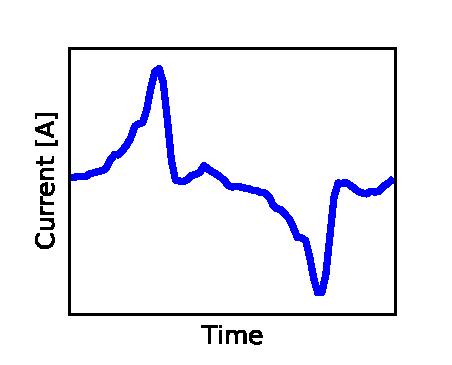
\includegraphics[width=0.45\linewidth]{bolt/comp_all18.eps} &   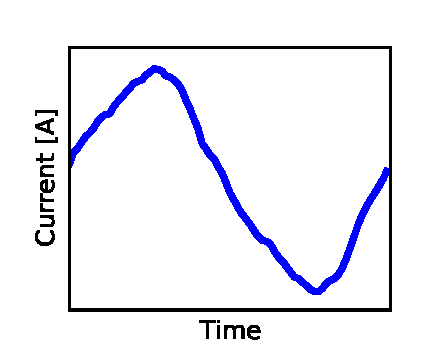
\includegraphics[width=0.45\linewidth]{bolt/comp_all78.eps} \\
(a) & (b) \\
 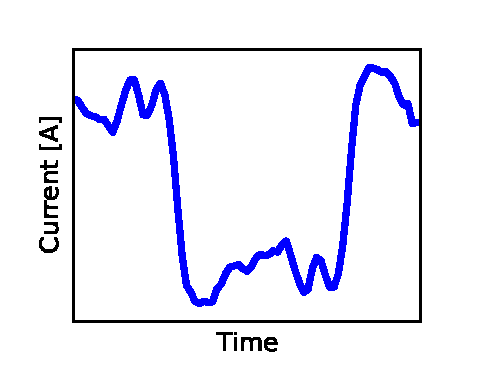
\includegraphics[width=0.45\linewidth]{bolt/comp_all1.eps} &   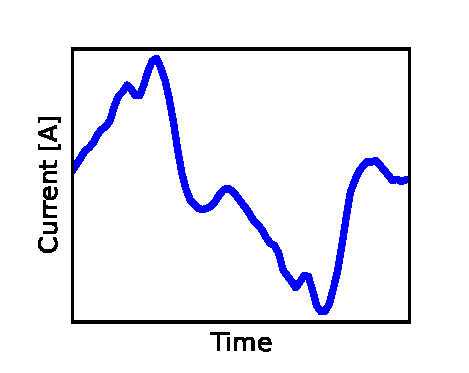
\includegraphics[width=0.45\linewidth]{bolt/comp_all26.eps} \\
(c)  & (d) \\
\end{tabular}
\caption[BOLT: Example inferred subcomponents extracted with BOLT.]{Four out of the 100 inferred subcomponents in the aggregate signal: (a) waveform of a power supply for a computer, (b) an almost purely resistive load, (c) highly reactive load, and (d) superposition of appliances}
\label{fg:wv}
\end{figure}

The weights between a binary unit and the linear output units (i.e., the columns of $G$) incorporate the information about the waveform of the corresponding component. Figure \ref{fg:wv} shows some of the inferred subcomponents identified in the aggregate signal after transforming them back into time-domain. Figure \ref{fg:wv} a) shows a waveform whose temporal activity is highly correlated with the activity of a computer. Computers like many other electronics are powered by a power supply unit (PSU) which transforms AC to DC current by rectification. The inferred waveform shows how the rectifier consumes power when the voltage peaks. We can also infer that the computer's PSU performs full-wave rectification as opposed to half-wave rectification in which case only single peak would be shown.\\

Figure \ref{fg:wv}b shows a generic sinusoidal waveform. Unfortunately, this waveform cannot easily be attributed to any specific appliance. In the experiment conducted on the BLUED dataset, the network infers 12 highly sinusoidal components, and for none of these their corresponding $X$ row correlates highly with any single appliance ground truth. This is most likely due to the fact that the network can use purely sinusoidal components as building blocks for purely resistive loads. For example, if there are two purely resistive loads consuming 200W and 250W respectively, the network has multiple equally valid solutions for decomposing their waveforms. In a perfect world, the network would allot one component to be a 200W sinusoidal and the other to be a 250W sinusoidal. This would readily disaggregate the energy of both appliances. However, the network could also explain the aggregate waveform by inferring one 200W sinusoidal and another 50W sinusoidal in which case non-linear re-aggregation of the inferred subcomponents is required to disaggregate the appliances.\\

Figure \ref{fg:wv} c) shows a component consuming solely reactive power. With very few exceptions, this component is almost always active during the whole duration of the dataset. The component does not consume any active power.\\

Figure \ref{fg:wv} d) shows a component with two peaks. The inferred component shows similarly high temporal correlation with the laptop and the desk lamp which suggests that the inferred component might be the superposition of those two appliances. The algorithm does not guarantee that the waveform of every inferred subcomponent is caused by a single appliance.

\begin{figure}
\begin{tabularx}{\textwidth}{XcXcX}
\noindent\parbox[c]{\hsize}{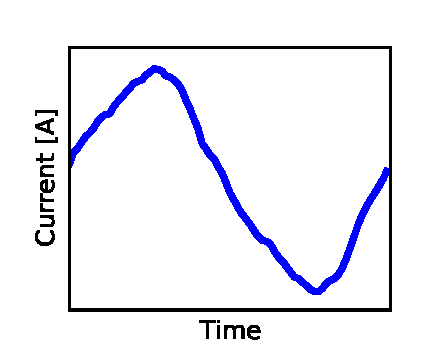
\includegraphics[width=0.75\linewidth]{bolt/comp_all78.eps}}  &+&  \noindent\parbox[c]{\hsize}{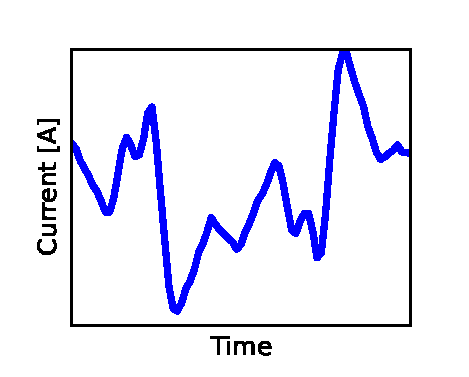
\includegraphics[width=0.75\linewidth]{bolt/comp_all5.eps}}   &=&  \noindent\parbox[c]{\hsize}{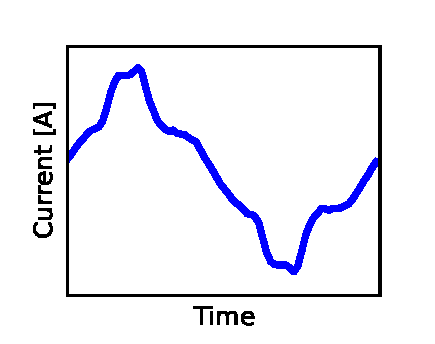
\includegraphics[width=0.75\linewidth]{bolt/sum70_5.eps}}
\end{tabularx}
\caption[BOLT: The sum of a seemingly noisy and a sinusoidal component.]{The sum of a seemingly noisy and a sinusoidal component.}
\label{fg:wv_sum}
\end{figure}

Figure \ref{fg:wv_sum} shows a seemingly noisy component. Even though the network is constrained in such a way that the power at line frequency must be greater than zero, the component exhibits negative power overall (assuming stable voltage at 110V), i.e. the component alone cannot represent an appliance. However, if this component is added to a sinusoid, the resulting component shows much structure and is similar to other inferred components. The seemingly noisy component can modify other components whose structure it can partially hijack. %The 'noisy component' could also be an indicator for a multi-state device whose waveform scales up with power consumption since it can take an arbitrary resistive load and shift its shape.\footnote{We are unable to verify this claim so far}\\

To sum up, the inferred subcomponents seem to be either: (a) the waveform of a specific appliance, (b) the superposition of the waveforms of multiple appliances, (c) modifier that requires the presence of another subcomponent, (d) a sinusoidal building block; or (e) a duplicate of another subcomponent.

\section{Combining Binary Components}
Following the intuition gained about the nature of the inferred subcomponents, supervised and unsupervised approaches for inferring appliance activity given the activities of inferred subcomponents will be discussed.\\
Let the matrix containing the activations of the inferred subcomponents be $X \in (0,1)^{d \times T}$, with $d$ being the number of components and $T$ the number of current and voltage cycles. The $t$th row of $X$ denotes the hidden states of the network $x(t)$ given input $y(t)$.

\begin{description}
\item[Supervised Re-Aggregation] In the supervised case, we also assume knowledge of a matrix containing ground truth of whether or not a specific appliance is turned on or off at any given voltage cycle. Let $G \in (0,1)^{T \times A}$ denote this matrix with $A$ being the number of appliances.
\item[Logistic Regression] An algorithm is sought that can model a binary response given predictors. Logistic regression can be used to predict the probability of binary probabilistic outcomes. We are interested in modeling $P(g_i (t) = 1 | x(t))$. Using logistic regression to model this distribution assumes that $P(g_i (t) = 1 | x(t))$ is a Bernoulli distribution with
\begin{align*}
P(g_i (t) = 1 | x(t)) = \frac{1}{1+exp[w_i^T x(t)]}
\end{align*}
 The model parameter $w_i$ can be obtained using a maximum likelihood estimate.
\item[Boolean Re-Aggregation] Logistic Regression learns a complex non-linear function but scenarios in which Logistic Regression can be applied without access to ground truth seem unlikely. Collecting ground truth requires sub-metering of appliances and is often prohibitively expensive. An unsupervised approach to re-aggregation will most likely analyze the temporal activity and the shape of the waveform of the inferred subcomponents and then combine subcomponents into appliances.\\
The temporal activity of a subcomponent, i.e. $x_j \in \{0,1\}^T$ (the columns of $X$), can be viewed as a sequence of truth values indicating if the respective component is active. Let $\lor$ be the element-wise $or$-operator such that $x_j \lor x_i \in \{0,1\}^T$. Since the network might infer the same component (according to its waveform) multiple times, a successful re-aggregation strategy would need to identify components with similar waveforms and connect them via the $\lor$-function.\\
Furthermore, imagine a scenario with two purely resistive appliances consuming 200W and 250W. As described earlier, the network could explain the aggregate waveforms by allocating one 200W sinusoid and one 50W sinusoid. Let $x_1$ and $x_2$ be the subcomponents constituting the inferred sinusoidal building blocks respectively. For the temporal activity pattern of the appliance consuming 250W, the following needs to be true: $x_1 \land x_2$, whereas for the appliance consuming 200W, we need to have $x_1 \land \neg  x_2$.\\
In order to provide an upper bound for an unsupervised algorithm that finds a boolean function connecting subcomponents, an algorithm is introduced that performs a greedy search over boolean functions in a supervised way: A function $f(x_j,...,x_k)$ is sought that maximizes the similarity between $g_i$ (the temporal activity of appliance $i$) and the output of that function on a subset of binary components $x_j,... ,x_k$. We furthermore assume that $f$ solely contains the operators $\lor, \land$ and $\neg \land$. As a similarity measure the F1 score is used.\\
The greedy algorithm iteratively adds one component to the function. The algorithm is initialized believing that $g_i$ is always turned on, i.e. $f_0 = (1)^T$. Then it iterates over all $x_i$ and computes the F1 score that would result in either appending $\land x_i$, $\lor x_i$ or $\land \neg x_i$ to $f$. After one sweep, the component that resulted in a maximal increase in F1 score is selected and appended to $f$. This is repeated until the F1 score cannot be improved further.
\end{description}
 
 \section{Unsupervised Re-Aggregation}
 \subsection{Lower bound on unsupervised Re-Aggregation}
 The assumption that every inferred subcomponent readily constitutes an appliance is a far-fetched assumption but can serve as a lower bound for unsupervised re-aggregation strategies. For each appliance, the component resulting in the highest F1 score compared to the ground truth is selected. This assumes that it is possible to classify subcomponent waveforms and their temporal activity patterns in order to infer appliances or receive this information from a user.
 
 \subsection{Na\"ive Re-Aggregation}
 When applying the supervised boolean re-aggregation described earlier, the algorithm seems to favor connecting subcomponents using the $\land$-operator. Following this intuition, a na\"ive re-aggregation strategy is introduced: two similarity metrics are defined: $d_w$ and $d_a$. The purpose of $d_w$ is to measure the similarity between the waveforms of two subcomponents, whereas $d_a$ measures the similarity between the temporal activity patterns of two subcomponents. We assume knowledge of a seed-component which in this case is the component resulting in the highest F1 score when comparing components to the ground truth. So ultimately, the goal is to improve the lower bound on unsupervised re-aggregation introduced earlier.\\
 For every appliance the seed-component is found using the ground truth. Let $x_{a,s}$ be the seed-component of appliances $a$. Then, for every component, a weighted sum of the similarity scores is computed: $d(x_{a,s}, x_i) = \lambda d_w(x_{a,s}, x_i) + (1-\lambda) d_a(x_{a,s}, x_i)$. Let $X_d$ be the set of components for which this similarity is bigger than a threshold $\epsilon$, i.e. $X_d(a) = \{x_i | d(x_{a,s}, x_i) > \epsilon\}$. All components in $X_d(a)$ are connected using the $\land$-operator, i.e. $\hat{g}_a = \bigwedge_{x_i \in X_d(a)} x_i$.
 
 \section{Results}
 \subsection{Supervised}
 In the supervised scenario, the power trace of the individual appliances can be estimated in a straight forward way if we assume that the $on$ and $off$ consumptions of appliances are known. Let $\hat{g}_a$ be the boolean time series representing the estimate for appliance $a$, then $\hat{p} = p_{on} \hat{g}_a  + p_{off}(1-\hat{g}_a)$. As a measurement of the goodness of the inferred power trace, the mean deviation error is employed: \begin{align*}
E(p, \hat{p}) = \sum_{i,t} \frac{|p_i(t) - \hat{p}_i(t)|}{p_i(t)}
\end{align*}

BOLT poses energy disaggregation as a waveform classification problem. Current waveforms are highly non-iid (independently and identically distributed), which poses a challenge for properly evaluating the performance. Thus, we evaluate the performance in two ways: first, we assume the current readings are iid and therefore randomly split matrix $X$ into a training and test set (50/50 split) for the logistic regression. This might, however, overestimate the performance in some cases but allows us to obtain disaggregation results for every appliance. Second, we perform \emph{snippet cross-validation}. For this, the ground truth is sliced into non-overlapping snippets that contain a single run-cycle of an appliance, i.e. the data is separated between an \emph{off} and an \emph{on}-transition such that every snippet contains a run-cycle and some examples where the appliance is off to ensure that no data is lost. The logistic regression is then trained on all but one snippet and evaluated on the snippet that it was not trained on. Note that such an evaluation is not possible for all appliances (e.g. those appliances that only contain a single run-cycle).
Table \ref{bolt:results} shows the results on the individual appliances for which ground truth data was available. The column ``active'' shows the proportion at which the appliance is active. Since the energy was estimated assuming 2-state appliances, \emph{mean disaggregation error} captures the variance of the appliances to some degree. A perfect 2-state prediction of an appliance with higher variance will always lead to a higher \emph{mean disaggregation error}, even though the energy in sliding windows (or power at a lower temporal resolution) would be predicted perfectly. The lower bound for assuming 2-state appliances and a perfect prediction is shown in the column $E(p)$. $E(\hat{p})$ and $E_S(\hat{p})$ shows the mean disaggregation error using iid- and snippet-evaluation, respectively.\\
Whether or not the algorithm can detect if an appliance is turned on or off was measured using the F1 score (0 - worst, 1 - best). As expected, for iid-evaluation, combining binary subcomponents using logistic regression ($F1_{L}$) outperforms the approach based on greedy search ($F1_{B}$). $F1_{S}$ shows the performance using snippet evaluation.\\
\begin{table}[]
\setlength{\tabcolsep}{1pt}
\centering
\begin{tabular}{l|c|c|c|c|c || c | c}
\hline
Appliance      & Active            & $F1_{B}$ & $F1_{L}$ & E($\hat{p}$) & E($p$) & $F1_{S}$ & $E_s(\hat{p})$ \\ \hline
A/V LR         & 60\%              & 0.89        & 0.98       & 0.04      & 0.009  & - & -\\
Computer 1     & 27.3\%            & 0.88        & 0.99       & 0.05      & 0.042 & 0.96 & 0.10  \\
Desk Lamp      & 21.4\%            & 0.84        & 0.95       & 0.06      & 0.013 & 0.81 & 0.38  \\
DVR            & 20.7\%            & 0.94          & 0.99       & 0.006      & 0.005 & 0.89 & 0.05  \\
Socket LR      & $>0.1\%$ & 0.96        & 0.92       & 0.09      & 0.089 & - & -  \\
Garage Door    & 0.4 \%            & 0.49          & 0.89       & 0.07      & 0.063 & - & -  \\
Iron           & 0.1 \%            & 0.74        & 0.92       & 0.12      & 0.115 & - & -   \\
Laptop 1       & 33.3\%            & 0.75        & 0.92       & 0.34      & 0.272 & - & -  \\
LCD Monitor    & 16.2\%            & 0.73        & 0.94       & 0.12      & 0.029 & 0.79 & 0.38  \\
Monitor 2      & 17.3\%            & 0.80        & 0.92       & 0.20      & 0.089 & - & -   \\
Printer        & 0.1\%             & 0.45           & 0.70       & 0.05      & 0.045 & - & -  \\
Tall Desk Lamp & 21.4\%            & 0.84        & 0.95       & 0.06      & 0.008 & 0.80 & 0.38  \\
TV Basement    & 20.7\%            & 0.94        & 0.99       & 0.05      & 0.029 & 0.88 & 0.26 \\ \hline
Random         & 30\%              & 0           & 0          & -         & -    & 0  & -   \\ \hline \hline
Overall        &                   &             &            & 0.058      & 0.037 & - & 0.18
\end{tabular}
\caption[BOLT: Supervised performance comparison]{``Active'' denotes the proportion during which the appliance was active, $F1_{B}$ and $F1_{L}$ show the performance of the Boolean Search and logistic regression in the iid-evaluation setting whereas $F1_{S}$ shows the performance of the logistic regression using snippet crossvalidation, $E(\hat{p})$ and $E(p)$ show mean disaggregation error of the inferred power trace (Logit) and the lower bound assuming 2-state appliances. $E_S(\hat{p})$ shows the same error using snippet crossvalidation. }
\label{bolt:results}
\end{table}


\begin{table}[]
\setlength{\tabcolsep}{3pt}
\centering
\begin{tabular}{lcc}
\hline
AV-LR  \\
 \includegraphics[width=20mm]{comps/comp_all63.pdf}        & \includegraphics[width=20mm]{comps/comp_all49.pdf}       & \includegraphics[width=20mm]{comps/comp_all23.pdf}   \\ \hline
Computer 1     \\
 \includegraphics[width=20mm]{comps/comp_all30.pdf}        & \includegraphics[width=20mm]{comps/comp_all60.pdf}       & 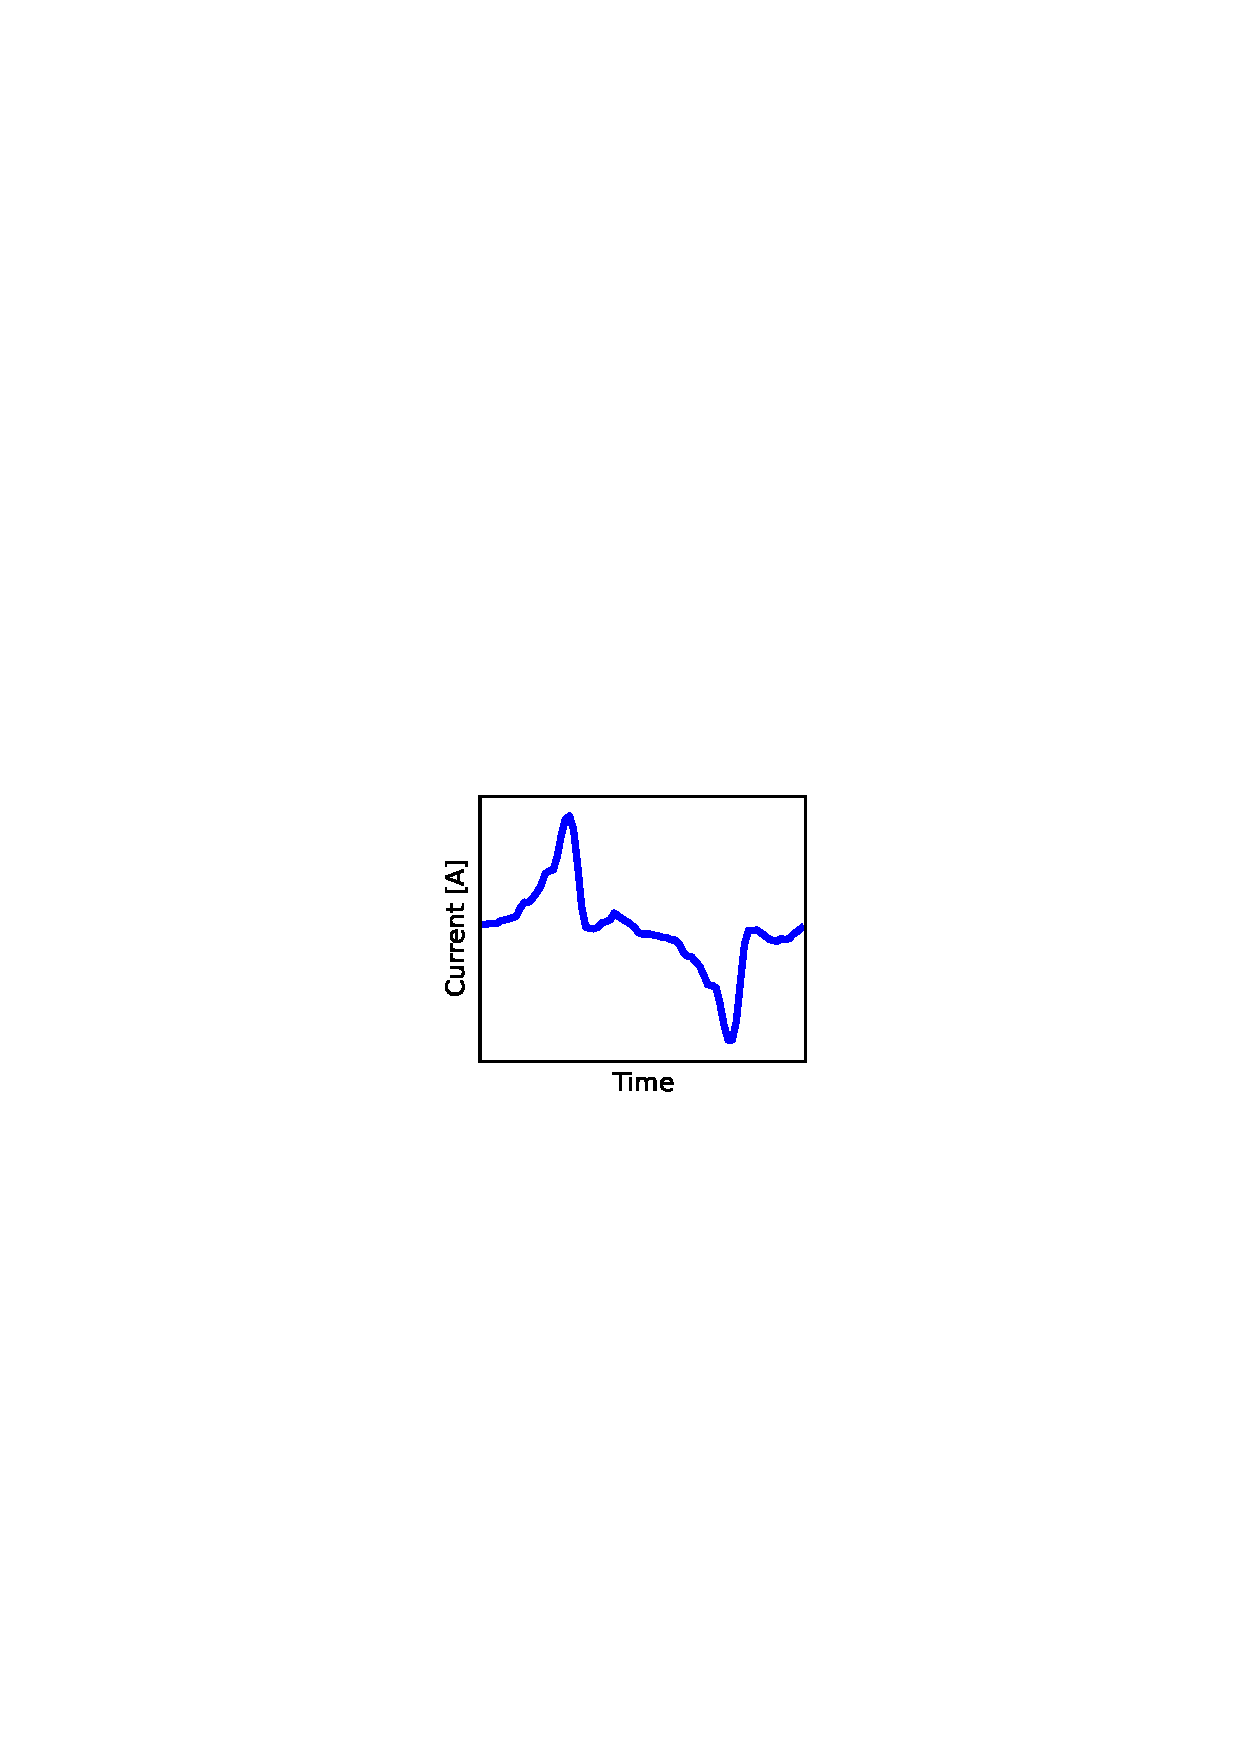
\includegraphics[width=20mm]{comps/comp_all18.pdf}   \\ \hline
DVR            \\
\includegraphics[width=20mm]{comps/comp_all34.pdf}        & \includegraphics[width=20mm]{comps/comp_all82.pdf}       & \includegraphics[width=20mm]{comps/comp_all47.pdf}   \\ \hline

Laptop 1     \\
\includegraphics[width=20mm]{comps/comp_all36.pdf}        & \includegraphics[width=20mm]{comps/comp_all69.pdf}       & \includegraphics[width=20mm]{comps/comp_all90.pdf}   \\ \hline

LCD Monitor  \\
\includegraphics[width=20mm]{comps/comp_all81.pdf}        & \includegraphics[width=20mm]{comps/comp_all30.pdf}       & \includegraphics[width=20mm]{comps/comp_all55.pdf}   \\ \hline
Monitor 2      \\
\includegraphics[width=20mm]{comps/comp_all97.pdf}        & \includegraphics[width=20mm]{comps/comp_all13.pdf}       & \includegraphics[width=20mm]{comps/comp_all50.pdf} 

\end{tabular}
\caption[BOLT: The components that contributed most to the disaggregation of the respective appliances.]{The components that contributed most to the disaggregation of the respective appliances.}
\label{waveforms}
\end{table}
The Boolean Re-Aggregation allows the recovery of the components which contributed most to the disaggregation of the appliances. Table \ref{waveforms} shows the three most influential components for some of the appliances excluding components that are connected by $\neg \land$, i.e. only appliances that have a positive influence on disaggregation. What is surprising is that, for example, the first waveform inferred for AV-LR seems to be more similar to the waveforms of the Computer than to its other waveforms. Since ground truth of the waveforms of the appliances is not available, it is unclear why this is the case. One possible explanation is that the algorithm exploited appliance co-variance information, i.e. if an appliance is only active when another appliance is active, the algorithm might learn the waveform of that other appliance.

\subsection{Unsupervised}
Table \ref{results_unsup} shows the results of the unsupervised approaches. The dataset is heavily biased towards some appliances, i.e. some appliances are active for just a fraction of the dataset. This bias seems to be reflected in the performance of the unsupervised disaggregation: only appliances that were active for at least 15\% achieved an F1 score of over 0.6. Even though the performance dropped substantially in comparison to the supervised case, it still seems to perform well in comparison to existing energy disaggregation algorithms. It is hard to compare different NILM systems since different algorithms are evaluated on different datasets. But to give an intuition on how well BOLT performs in comparison to other systems, we compared BOLT to the algorithm proposed in \cite{jiafully}. In \cite{jiafully} a disaggregation system based on non-parametric FHMMs is introduced and evaluated on the REDD \cite{kolter2011redd} dataset. REDD is of comparable complexity but the high-frequency portion of the dataset is compressed in a lossy way which might have a detrimental effect on the performance of BOLT. Their proposed method based on NFHMM achieves a score of 0.25 (GSPA, 0 worst, 1 best) on the REDD dataset in comparison to 0.61 unsupervised BOLT on the BLUED dataset.\\
For the na\"ive unsupervised re-aggregation, the optimal parameters $\lambda$ and $\epsilon$ were obtained for every appliance using cross-validation. The na\"ive unsupervised re-aggregation was only able to slightly improve the performance on a small subset of the appliances but it shows that it seems to be possible to further improve the unsupervised approach.

\begin{table}[]
\setlength{\tabcolsep}{3pt}
\centering
\begin{tabular}{lccccc}
\hline
Appliance      & Active            & Lower Bound F1 & Na\"ive F1 \\ \hline
A/V LR         & 60\%              & 0.85        & 0.85         \\
Computer 1     & 27.3\%            & 0.67        & 0.74      \\
Desk Lamp      & 21.4\%            & 0.70        & 0.70     \\
DVR            & 20.7\%            & 0.85         & 0.85      \\
Socket LR      & $>0.1\%$ & 0.0       & 0.0      \\
Garage Door    & 0.4 \%            & 0.24          & 0.3  \\
Iron           & 0.1 \%            & 0.09        & 0.30   \\
Laptop 1       & 33.3\%            & 0.71        & 0.71   \\
LCD Monitor    & 16.2\%            & 0.63        & 0.63  \\
Monitor 2      & 17.3\%            & 0.67        & 0.70  \\
Printer        & 0.1\%             & 0.07           & 0.07 \\
Tall Desk Lamp & 21.4\%            & 0.70        & 0.70   \\
TV Basement    & 20.7\%            & 0.85        & 0.85   \\ \hline
\end{tabular}
\caption[BOLT: Unsupervised performance comparison]{ ``Lower Bound F1'' and ``Na\"ive F1'' show the performance using different unsupervised reaggregation techniques.}
\label{results_unsup}
\end{table}

\newpage
\section{Hardware Implementation}

\begin{figure}[!ht]
\includegraphics[width=0.85\linewidth]{bolt/OEM.jpg}
\caption[BOLT: The OpenEnergyMonitor setup.]{1.) Voltage Input, 2.) Power Supply, 3.) Current Transformer 4.) OpenEnergyMonitor 5.) Metered Power Strip }
\label{fg:oem}
\end{figure}

NILM systems that rely on high sampling rates of the current or voltage signal quickly run into data transmission and storage problems. For example, a system which carries out inference on a centralized server and that requires a sampling rate of 12kHz would need to transmit and store approximately 4GB per sensor day assuming a sensor resolution of 16bits per sample. Such a system would not scale well to many sensors (or buildings). \ourname, however, can infer the states of the subcomponents directly and then only transmit these states. Since the states of the subcomponents can be encoded by a single bit per subcomponent, inferring the subcomponents can be viewed as very strong compression and, as we have shown earlier, this compression preserves the information of appliance activities. By doing so, the data that needs to be transmitted can be reduced to 8.5MB per sensor/day, resulting in a 500 fold reduction.\\
Ultimately, the data that needs to be transmitted is independent of the internal sampling frequency and only depends on the number of subcomponents. This means that theoretically, megahertz sampling frequencies could be leveraged while still keeping the data transmission and storage costs low. However practically, with increasing internal sampling frequency, the computational burden increases which in turn requires computationally more powerful smart-metering hardware.\\
We conducted an experiment to show the maximum sampling rates achievable with a Raspberry Pi 2\footnote{http://raspberrypi.org}. Figure \ref{fg:oem} shows a picture of the experimental setup. The Raspberry Pi is a ubiquitous, low-cost (US \$35) embedded computing platform powered by a 900MHz quad-core ARM Cortex-A7. The open source Open Energy Monitor\footnote{http://openenergymonitor.org} was used for our experiments. The Raspberry Pi built into the Open Energy Monitor is internally connected to a micro-controller powered by an ATMega328p with an internal clock rate of 16MHz which serves as a sensing relay.

\begin{figure}[!ht]
\centering
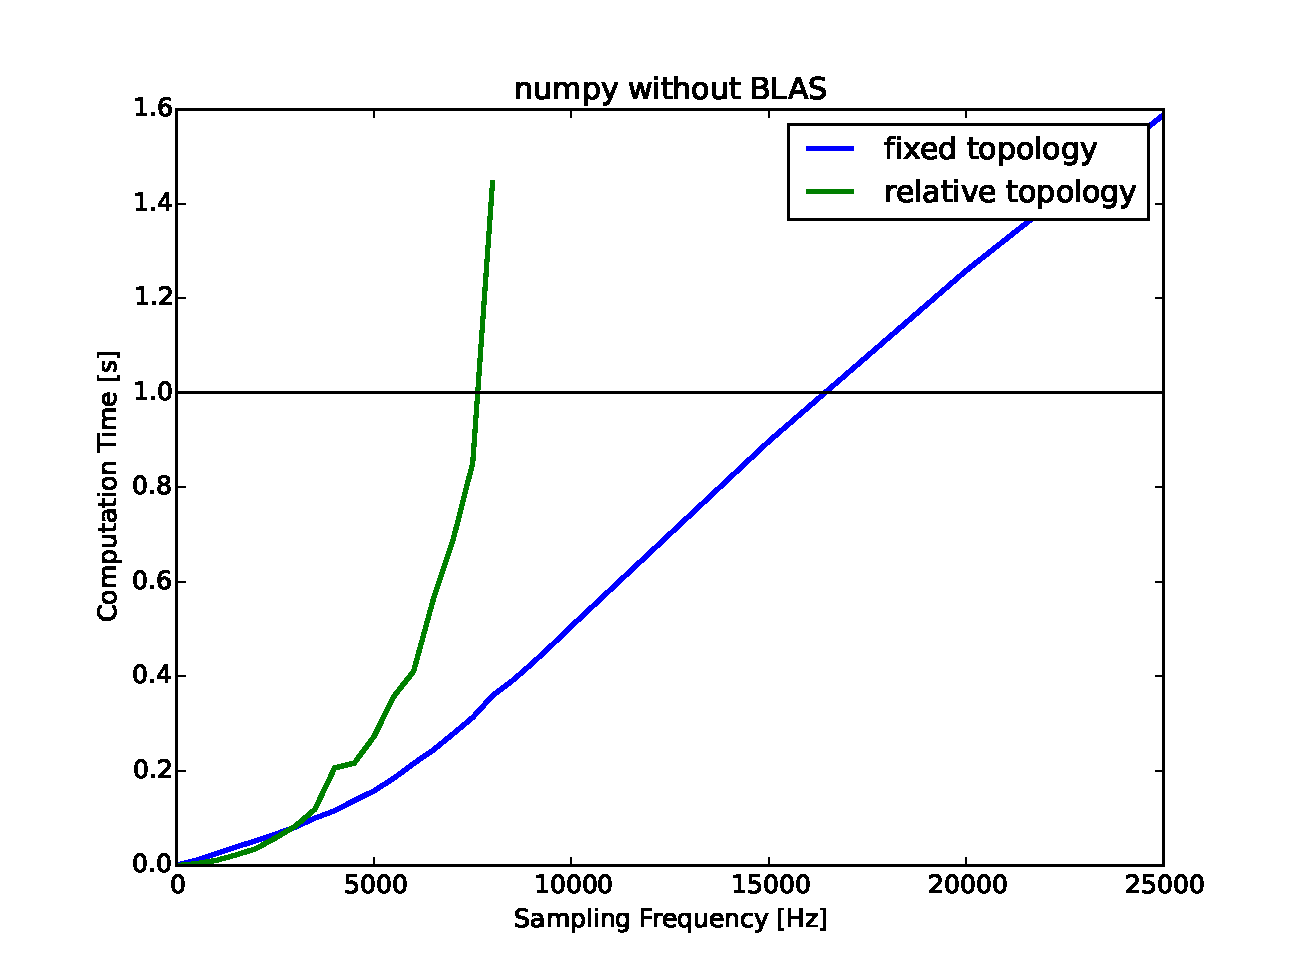
\includegraphics[width=0.75\linewidth]{bolt/sampling_freq.eps}
\includegraphics[width=0.75\linewidth]{bolt/sampling_freq_blas.eps}
\caption[BOLT: Computational time as a function of the sampling rate.]{The computational time as a function of the sampling rate. The top figure assumes a simple numpy implementation whereas the bottom figure uses numpy and BLAS. The black horizontal line marks up until when real time inference is possible.}
\label{fig_imp}
\end{figure}

The computational cost of inferring the states of the subcomponents is a function of the number of computational nodes in the network and by increasing the sampling frequency, at the very least, the number of the computational nodes in the input layer increases. In order to investigate the limits of real-time inference as a function of the sampling rate two sets of experiments were conducted. In the first experiment a fixed topology of the network is assumed: Let $f$ be the sampling rate. The topology of the network is in the first experiment: $f \rightarrow 500 \rightarrow 100 \rightarrow f$, i.e. there are $f$ input neurons that project the input onto a hidden layer consisting of 500 neurons which in turn projects the input down onto 100 binary units. The states of the binary units in turn are used to recreate the input, i.e. the output dimensionality is also $f$. In the second experiment, we considered a network whose topology grows linearly with the sampling rate. Data with a higher sampling rate might contain more structure and in turn require more flexibility of the network to disaggregate the waveforms. The topology of the `relative network' is set to: $f \rightarrow f/10 \rightarrow 100 \rightarrow f$. Inference is carried out with an implementation using the Python package numpy. Since inference in neural networks can be implemented by a succession of matrix-multiplications followed by the application of a non-linearity, the potential speed-up by using BLAS (Basic Linear Algebra Subprograms\footnote{http://www.netlib.org/blas/}) is also investigated.\\
Note that with a simple trick, the costs of having to transform the inputs into frequency domain during inference, i.e. the costs of the FFT can be avoided by exploiting the linearity of the matrix-multiplications and FFT. Let $y(t)$ be the input at time $t$ and $w$ be the first column of the weights coming into the first layer. Let $\mathcal{F}$ denote the Fourier transform, i.e. $\mathcal{F}(y(t))_k = \sum_{j=0}^N exp(-2\pi jk/N)y(t)_j$. For the activation of the first neuron in the first layer before applying the non-linearity the following holds: 
\begin{align*}
\mathcal{F}(y(t))^Tw &=\sum_{k=0}^N w_k \sum_{j=0}^N exp(-2\pi jk/N)y(t)_j\\
 &=\sum_{k=0}^N y(t)_k \sum_{j=0}^N exp(-2\pi jk/N) w_j = \mathcal{F}(w)^Ty(t)
\end{align*}
 This ultimately means that instead of computing the Fourier Transform of every input, instead the Fourier transform of the weight-matrix can be computed once leading to a substantial decrease in computational cost. Training the network in frequency-domain and doing inference in time-domain allows for enforcing frequency-constraints while at the same time keeping the computational time needed for inference low.\\
Figure \ref{fig_imp} shows the increase in computational time as a function of the sampling rate for the topologies described above. The top figure shows the inference time using a simple numpy implementation whereas the bottom figure shows a numpy implementation using BLAS. The sampling frequency describes the data collected within 1 second and as long as the data collected can be processed in less than 1s, real time inference is possible on the smart meter. It can be seen that when using a fixed topology, real-time inference using BLAS is possible up until sampling rates of 55kHz. But as we have shown earlier, even a sampling rate of only 4.8kHz suffices to infer appliance states with high precision.

\section{Conclusion}

The approach introduced in this paper seems to be the first approach that acknowledges the fact that loads are not necessarily linear, i.e. not all loads are phase-shifted sinusoids. Most approaches simply use active and reactive power as features and neglect the fact that some appliances have very distinct waveforms which cannot be characterized in the traditional resistive, inductive and capacitive load trichotomy. Applying Binary Matrix Factorization in order to infer reoccurring additive subcomponents in the current signal allows to decompose the current signal and extract a very rich set of features: component waveforms. Combining the inferred components to ultimately infer whether or not an appliance is active has shown great potential. The supervised case approaches what is theoretically possible under the assumption of 2-state appliances but requires the availability of training data whereas the results of unsupervised approaches indicate the possibility of re-aggregating appliances in an unsupervised way.\\ The approach introduced in this paper also shows advantages from a computation point of view: the hidden state given some input can be viewed as a drastically compressed representation of the input that preserves information about which appliances are active and, since inference of the hidden states using the neural network is computationally cheap, only the hidden states (component states) need to be transmitted, which in turn reduces the data storage and transmission burden while still leveraging high-frequency information. For instance, an approach that requires remote inference and a sampling frequency of 12kHz would need to send out 96kb/s as opposed to 16byte/s (100bits per component + 32bits for the aggregate signal) using this approach. Additionally, inferring which appliances are active at any given time requires only a 1 second slice of current, which in turn implies that inference can be carried out without the need of a warm-up phase such as those required by approaches based on FHMM.

\section{Future work}

Some machine learning systems such as, for example, a system that predicts the future value of a random variable in can continuously learn from its mistakes. In order to obtain the information of whether or not a past prediction was right or wrong, simply time needs to pass and the correct value can be observed. In this respect, NILM systems face an additional difficulty: a purely non-intrusive system can never learn from its mistakes because it cannot observe the true state of appliances. This characteristic is detrimental for supervised approaches that assume snapshot knowledge of appliances because, implicitly, these approaches also assume that loads do not change over time. For unsupervised approaches, this means that the entire NILM system can only be evaluated on a minuscule subset of homes which are submetered and buildings for which the systems performs suboptimally can at most only tried to be identified by indirect metrics. Because of the unsupervised nature of the subcomponent identification step of the system introduced in this paper, continuous retraining of the system is possible. However, combining the subcomponents into appliances still requires training to allow for high precision disaggregation. The requirement for training can, nonetheless, be alleviated. Two strategies that might alleviate the need for ground truth will be discussed here in more detail.
\begin{description}
\item[Sparse Coding and Waveform Library] As we have discussed earlier, especially in the unsupervised case, the proposed system struggles with purely resistive loads as they lack discriminative features. The algorithm can always stitch together and re-use sinusoids. This problem could however be alleviated by enforcing sparsity of the binary hidden layer of the neural network. If the algorithm stitches sinusoids together, more subcomponents are active in comparison to a scenario in which each subcomponent represents an appliance. This is why the effect of enforcing sparsity in the hidden layer of the neural network might be worth investigating.\\
Enforcing sparsity in the hidden layer is closely linked with infusing prior knowledge into the system. If knowledge about the appliances present in a building is assumed, this knowledge could be used to alleviate the need for ground truth. In case the waveforms of the appliance are known, i.e. the algorithm can access a waveform library that contains the waveforms of individual appliances, a prior distribution over the weights coming into the output layer (the component waveforms) could be imposed in order to enforce that the component waveforms are similar to the elements in the waveform library.
\item[Distributed Sensing] Another way to alleviate the need for ground truth is to build a hybrid approach. For some chain franchises like e.g. fast food restaurants, gas stations, supermarkets, etc. the assumption that loads are similar across different buildings might be valid. This could be leveraged by submetering a subset of the franchise locations and broadcasting the appliance specifics knowledge from the submetered to the non-submetered locations. BOLT seems to be a prime candidate for such a strategy since the subcomponent identification portion of the algorithm is unsupervised. This allows to fuse the data collected at all franchise locations into a single stream of data. This stream of data can then in turn be used to train the unsupervised neural network model. In order to infer appliance states of non-submetered locations, the data at the submetered locations can be leveraged to create a supervised model which is then shared with the non-submetered locations. Such a strategy has many advantages over traditional NILM systems: 
\begin{itemize}
\item Continuous re-training allows handling of load patterns that might change over time
\item Potentially high precision NILM while still bringing down the costs substantially - only a small subset locations would need to be submetered
\item Training a joint unsupervised model of all franchise locations allows to incorporate information of non-submetered locations into the modeling process which might make the overall system very robust
\item Deep Learning seems to thrive on big datasets and in such a scenario BOLT could in principle leverage the information of an infinite data stream
\end{itemize}
Such a distributed NILM system however creates new challenges. For example, the system needs to communicate information between different smart meters extensively. Whether BOLT can be used to reduce the data transmission requirements is an interesting future research direction, especially as technologies like Low Power Wide Area Networks (LP-WAN) become more widespread.
\end{description}

\section{Postamble}
This publication introduces an algorithm to obtain appliance state estimates solely based on information present within a single cycle of current. The algorithm approximates an otherwise NP-hard problem by estimating the gradient through the Heaviside non-linearity. The publication answers Research Question 1.1.1, because inference requires only a forward pass through a neural network and can be carried out in real-time on embedded hardware, therefore fulfilling the additional requirement of computational efficiency. Furthermore, Research Question 1.1.2 is answered by evaluating the performance in a supervised and unsupervised fashion. In a supervised setting, the algorithm shows competitive performance in terms of disaggregation error. However, note that the performance drops considerably in an unsupervised setting.\\
In order to achieve computational efficiency, any temporal regularization that is usually present in state-based NILM approaches is ignored. Because of this BOLT seems to overfit, i.e. the algorithm finds solutions that are not constrained enough. Specifically, when a single appliance changes its state, the state of multiple components switch. Note that enforcing temporal regularization is computationally expensive because it requires an approximation of the filtering recursion. In the next chapter, an algorithm is presented that makes use of Variational Inference to achieve this.

\chapter{VarBOLT: Approximate Learning in Factorial HMMs}
The following publication can be viewed as an extension of BOLT. Specifically, it tries to overcome the problem that BOLT requires supervision in order to achieve competitive disaggregation results. In order to achieve this, temporal dependencies between appliance states are modeled which in turn requires an approximation of the filtering recursion, i.e. the publication tries to answers the question what a computationally efficient algorithm to approximate the filtering distribution to ultimately achieve temporal regularization is. Furthermore, the performance of the resulting algorithm is evaluated in an unsupervised fashion.

Lange, Henning, and Mario Berges. "Variational BOLT: Approximate Learning in Factorial Hidden Markov Models with Application to Energy Disaggregation." \emph{Thirty-Second AAAI Conference on Artificial Intelligence. 2018.}

\label{chapter:varbolt}

\subsection{Abstract}
The learning problem for Factorial Hidden Markov Models with discrete and multi-variate latent variables remains a challenge. Inference of the latent variables required for the E-step of Expectation Minimization algorithms is usually computationally intractable. In this paper we propose a variational learning approach mimicking the Baum-Welch algorithm. By approximating the filtering distribution with a variational distribution parameterized by a recurrent neural network, the computational complexity of the learning problem as a function of the number of hidden states can be reduced to quasilinear instead of quadratic time as required by traditional algorithms such as Baum-Welch whilst making minimal independence assumptions. We evaluate the performance of the resulting algorithm, which we call Variational BOLT, in the context of unsupervised end-to-end energy disaggregation. Specifically, we conduct experiments on the publicly available REDD dataset and show competitive results when compared with a supervised inference approach and state-of-the-art results in an unsupervised setting.


\subsection{Introduction}
Because of its potential to discover and unlock energy saving opportunities in buildings, the problem of energy disaggregation~\cite{hart1992} has received increased interest from various academic communities. The objective of this single-channel source separation problem, also known as non-intrusive load monitoring (NILM), is to infer appliance-level power consumption information given data from only a single sensing point at the main electrical panel of a building. The observed aggregate power measured at the main panel constitutes the sum of the power of the individual appliances. Since, appliance states (e.g., {\em on}, {\em off}) can be assumed to evolve independently and the aggregate observation is dependent on the joint state of all appliances, Factorial Hidden Markov Models (FHMM)~\cite{ghahramani1997factorial} have emerged as a prominent model for the generative process of the aggregate observations. However, because latent states become conditionally dependent given the observations, exact inference of the posterior, i.e. the distribution of appliance states given the aggregate observation, is assumed to be intractable. Numerous approximate inference techniques have been proposed and employed in the past to tackle this problem. Authors in~\cite{kolter2012fhmm} introduced the one-at-a-time constraint that postulates that only a single appliance can change its state at any given time. This constraint allows for posterior inference by either posing the problem as an integer programming problem~\cite{kolter2012fhmm} or by truncating the Viterbi algorithm~\cite{lange2016efficient}. However, these approaches were focused on the decoding rather than the learning problem. On the other hand, ~\cite{jia2015fully} proposed a solution to the learning problem based on MCMC sampling but this approach seems to struggle with slow mixing of the posterior.\\
The model introduced in this paper makes use of a highly tractable auxiliary distribution that approximates the true filtering distribution. This tractable distribution is parameterized by a deep recurrent neural network, specifically stacked LSTMs~\cite{hochreiter1997long}. We build on recent results showing how neural networks in conjunction with Variational Inference can be used as a powerful tool for statistical inference~\cite{kingma2013auto}. This combination is favorable because Variational Inference allows one to pose statistical inference as a (non-linear) optimization problem and neural networks have become a dominant approach for non-linear optimization.\\
Because we assume the latent variables to be binary (i.e. a Bernoulli auxiliary distribution) we face the additional difficulty of dealing with non-conjugate discrete distributions, which pose significant challenges in the context of neural networks and variational inference \cite{kingma2013auto}. As we will show later, this problem is circumvented by directly approximating the expectation of the true filtering distribution and introducing a loss function that directly penalizes the neural network outputs for deviating from that approximation. By making use of a tractable auxiliary distribution and making minimal independence assumptions (i.e. only posterior independence of the latent variables at a single time point) computations required for the filtering distribution that are typically quadratic in the number of hidden states can be reduced to quasilinear time. This ultimately allows modeling rich temporal dependencies between latent variables whilst keeping computational costs low. Although we focus on the application of energy disaggregation in this paper, our proposed method could find applications in other fields where FHMMs with binary latent states are employed such as in certain Bioinformatics problems, e.g., \cite{stanculescu2014hierarchical,asif2011large}.\\
The decreased computational costs for inference afford our solution with the additional advantage of addressing security and privacy concerns associated with energy disaggregation solutions. In other words, disaggregation can, in principle, be carried out in real-time on cheap off-the-shelf embedded hardware located within the premises.\\
In the next subsection, we introduce Factorial Hidden Markov Models and explain the need for variational approximation of the filtering distribution. The subsection that follows shows how variational estimates of the filtering distribution can be obtained efficiently. The next subsection highlights the importance of modeling temporal dependencies and shows how this can be achieved by additionally modeling the difference signal of the aggregate observations. We then present experiments/results on the REDD dataset and conclusions.

\subsection{Factorial Hidden Markov Models and Variational Inference}

\begin{figure*}[h]
\centering
\includegraphics[width=0.95\textwidth]{varbolt/matrixX_rev.pdf}\\
\includegraphics[width=0.45\textwidth]{varbolt/matrixW.pdf}
\includegraphics[width=0.45\textwidth]{varbolt/FHMM.png}
  \caption[VarBOLT: Aggregate instantaneous power waveforms and extracted candidate waveforms.]{(a): Matrix $X$ containing aggregate instantaneous power waveforms alongside the aggregate power. (b): Matrix $W$ containing candidate component waveforms. (c): Representation of a Factorial Hidden Markov model}
\end{figure*}

%$\mathfrak{z}_i$
FHMMs are a generalization of Hidden Markov Models in which multiple hidden states evolve independently in parallel. See Figure 1c for a representation of the associated graphical model. When the parameters of the individual HMM chains are known, energy disaggregation can be posed as the decoding problem for FHMMs. However, obtaining these paramaters is usually prohibitively expensive. On the other hand, unsupervised energy disaggregation can be posed as the learning problem on this graphical model.\\
Because of its factorial nature, the probability of the observation at time $t$, $x_t$, is a function of the joint hidden state $z_t$, with $t \in \{1,...,T\}$. In general, the latent variables of FHMMs are modeled as categorical variables, which could lead to computationally tractable solutions (e.g., \cite{jang2016categorical}). In our case we restrict $z_t$ to be binary, specifically Bernoulli distributed. Assuming binary hidden states removes some of the ambiguity inherent to the learning problem: every latent representation with categorical variables can be decomposed into a representation with binary variables, i.e. by assigning a binary variable for each categorical state. This binary decomposition is unique and in a sense maximal. However, binary decompositions can be aggregated into exponentially-many categorical decompositions, i.e. any combination of binary latent variables can be joined into one categorical variable. In order to avoid this ambiguity, we restrict the latent variables to be binary.\\
Since hidden states are assumed to be binary and multiple hidden states evolve in parallel, $z_t \in Z  = \{0,1\}^C$ with $C$ being the number of parallel hidden chains. Thus, the joint likelihood can be expressed as:
\begin{align}
p(x_{1:T},z_{1:T}) = \prod_t^T p(x_t|z_t)\prod_i^C p(z_{t,i}|z_{t-1,i})p(z_{0,i})
\end{align}

For the application of energy disaggregation, we choose a representation of the aggregate observation similar to our prior work~\cite{lange2016bolt}, i.e. the observation $x_t$ constitutes the aggregate instantaneous power waveform aligned by zero-crossings detected in the voltage line, thus $x_t \in \mathbb{R}^N$ with $N$ being the number of samples per voltage cycle. Figure 1a shows aggregate instantaneous power waveforms alongside the observed aggregate active power over time. Since instantaneous power is additive, we model $p(x_t|z_t)$ to be a Gaussian distribution with $p(x_t|z_t) = \mathcal{N}(x_t | Wz_t, \alpha I)$ where $\alpha$ is a variance parameter, $W \in \mathbb{R}^{N \times C}$ is a matrix containing the power waveforms of the inferred components and is not assumed to be known. Figure 1b shows an example of inferred power waveforms.\\
Baum-Welch, an Expectaction-Maximization algorithm, is a prominent algorithm for the learning problem in Hidden Markov Models. Baum-Welch makes model updates based on the expected time spent in states, the expected number of state transitions and the expected number of times a state emits an observation. An efficient algorithm to compute these quantities is the forward-backward algorithm. The forward-probabilities (2) can be computed recursively. Given the forward probabilities, the filtering distribution can be computed according to (3).
%\begin{equation}
\begin{align}
p(x_{1:t},z_t) &= p(x_t|z_t) \sum_{z' \in Z} p(z_t|z') p(z_{t-1}, x_{1:t-1})\\
p(z_t|x_{1:t}) &= \frac{p(x_{1:t},z_t)}{\sum_{z' \in Z} p(x_{1:t},z')}
\end{align}
%\end{equation}
Because the number of possible latent states $z$ grows exponentially with the number of components, evaluating (2) is intractable for FHMMs. However, as we will show later, ideas from Variational Inference can be used to approximate forward-probabilities.\\
 Variational Inference is a tool to deal with intractable posterior distributions and relies on an auxiliary or variational distribution $Q$ governed by the variational parameter $\Theta$. Posterior inference in $Q$ is required to be tractable, which is usually achieved by making independence assumptions. To paraphrase the main idea behind Variational Inference: in order to perform inference on a distribution $P$ with intractable posterior, variational parameters $\Theta$ are chosen in such a way that $Q$ best approximates $P$ and then inference is performed on $Q$ instead of $P$. For our application, $P$ is the filtering distribution, i.e. (3), and we choose $Q$ to be an independent multivariate Bernoulli distribution with density $q_\sigma(z_t) = \prod_i^C \sigma_i^{z_{t,i}}(1-\sigma_i)^{1-z_{t,i}}$ and with $\sigma_i$ being the coin-flip probabilities of the latent variables. For the conditional $q_\sigma(z_t|x_t)$, we assume the coin-flip probabilities to be functions of the conditioning variable $x_t$, i.e. $q_\sigma(z_{t} =\vec{1}|x_t) = \sigma_{t} = f_\Theta(x_t)$. Because we want $Q$ to capture the temporal dependencies present in $P$, we chose $f$ to be a recurrent deep neural network governed by the variational parameters $\Theta$ (which in this case constitute the weights of the neural network). This in turn means that $\sigma_t = f_\Theta(x_{1:t})$ is a function of all previous observations $x_{1:t}$, i.e. $Q$ is also a filtering distribution: $q(z_t|x_{1:t})$. Note that this implies that the auxiliary distribution does not assume temporal independence between latent variables but assumes independence between elements of the latent variable at any given time.\\
The evidence lower bound (ELBO) as a variational objective can be derived as follows~\cite{blei2011variational}:
\begin{align}
\mathcal{L} &= \log p(x_{1:t}) - D_{KL}(q(z_{t}|x_{1:t}) || p(z_{t}|x_{1:t}))\\
&=  \mathbb{E}_{Q}[\log p(x_{1:t},z_{t})] - \mathbb{E}_{Q}[\log q(z_{t})]
\end{align}
Note that because of the equivalence of (4) and (5), maximizing (5) is equivalent to maximizing (4). This means that optimizing the parameters of $P$ and $Q$ w.r.t. to (5) leads to maximization of the log-likelihood of the data as well as minimization of the posterior divergence. Although the second expectation of (5) usually has an analytical solution, evaluating the first expectation is usually achieved by sampling from $Q$. However, approximating the expression by sampling disconnects the optimization problem from the variational parameters $\Theta$, i.e. $Q$ vanishes from the optimization problem. For some continuous non-conjugate distributions, this problem can be avoided by the re-parameterization trick, i.e. by finding a deterministic and differentiable function that provides samples of $Q$ given the variational parameters $\Theta$ and some random noise. For binary non-conjugate distributions such as the Bernoulli such a function does not seem to exist~\cite{kingma2013auto}.\\
We circumvent this problem by approximating the true filtering distribution, i.e. estimate $\hat{p}(z_{t}|x_{1:t})$ with the help of $Q$. Given estimates $\hat{p}(z_{t}|x_{1:t})$, the $\sigma^*$ as a function of $\Theta$ resulting in the lowest forward KL-divergence can be obtained, i.e. $\sigma^* = \arg \min_{\sigma}\sum_t D_{KL}(\hat{p}(z_{t}|x_{1:t}) || q_\sigma(z_{t}|x_{1:t}))$. Given $\sigma^*$, the binary cross-entropy loss between $\sigma$ and $\sigma^*$ ($H(\sigma_t, \sigma_t^*)$) is then minimized in order to minimize the forward KL-divergence of the posterior.\\
Minimizing the binary cross-entropy loss between $\sigma$ and $\sigma^*$ minimizes the posterior divergence but since the parameters of $P$ (the component waveforms $W$) are not known, the model needs to be forced to explain the aggregate signal explicitly. Otherwise the free parameter $W$ will be abused to minimize the divergence without explaining the data. Thus, we additionally maximize $\mathbb{E}_{Q}[\hat{p}(z_t, x_{1:t})]$ in order to explain the aggregate waveforms. Hence, the objective function becomes:
\begin{align*}
L(\sigma, W) &=  \sum_t\mathbb{E}_Q[\hat{p}(z_t, x_{1:t})] - H(\sigma_t, \sigma_t^*)\\
\text{with:\ \ } \sigma_t^* &= \min_{\sigma}D_{KL}(\hat{p}(z_{t}|x_{1:t}) || q(z_{t}|x_{1:t})) \\
 &= \mathbb{E}_{\hat{p}(z_{t}|x_{1:t})}[z] \\
\text{and:\ \ } -H(\sigma_t, \sigma_t^*) &= \sigma_t^*\log(\sigma_t) + (1-\sigma_t^*)\log(1-\sigma_t) \\
\end{align*}
To sum up the main ideas of this paper:
\begin{itemize}
\item Computing the filtering recursion required for the E-step of Baum-Welch is prohibitively expensive since it requires a summation over exponentially-many latent configurations.
\item An auxiliary distribution $q(z_t|x_{1:t})$ that assumes independence between elements in $z_t$ is introduced, which allows for approximating $\hat{p}(z_t|x_{1:t})$. Note that $q$ does not assume independence over time steps. The independence structure of the auxiliary distribution is then exploited to approximate the filtering recursion efficiently circumventing summation of exponentially-many latent configurations.
\item In order to optimize the parameters of the auxiliary distribution, the variational parameters minimizing the KL-divergence between $P$ and $Q$, i.e. $\sigma^*$, are estimated and the binary cross-entropy loss between the predicted parameters $\sigma$ and the optimal $\sigma^*$ is minimized. As we will show later, this is equivalent to minimizing the KL-divergence but circumvents the re-parameterization trick and allows for a compact representation of the problem.
\end{itemize}
Note that we interchangeably call $\sigma$ and $\Theta$ variational parameters. However, in reality, $\sigma$ is a function of the true variational parameters, i.e. the neural network weights $\Theta$, and when a loss is defined w.r.t. $\sigma$ gradients w.r.t. $\Theta$ can be obtained by application of the chain rule, i.e. back-propagation.\\
In the next subsection, we will discuss how to obtain estimates of the filtering distribution probabilities, i.e. $\hat{p}(z_t|x_{1:t})$.

\subsection{Estimating filter distribution probabilities}
\label{sec:esti}
When using the forward-algorithm to obtain the filtering distribution $p(z_{t}|x_{1:t})$ for FHMMs, the computational complexity is in $\mathcal{O}(2^{2C}T')$ with $C$ being the number of components and $T'$ being the number of discrete time steps. In this work, we propose a learning algorithm that operates in $\mathcal{O}(C^{\epsilon+1}T)$ with $C^\epsilon$ being the number of candidate latent state configurations being considered and $T \ll T'$ (by reducing decision variables) and $\epsilon < C$ (by enforcing sparsity).
\subsubsection{Reducing decision variables}
For the problem of energy disaggregation, the aggregate observation is highly non-iid, i.e. instantaneous power waveforms tend to repeat themselves over time since they are associated with the operational state of appliances (and these do not change very often). This implies that, as long as the aggregate observations have not changed significantly, the latent states will not have changed and no new decision needs to be made. Thus, by employing a simple change-point detector that extracts points in time, so called events, where a significant change in the aggregate power was observed, the number of decision variables can be reduced significantly. Let the number of detected events be $T$. Reducing the number of decision variables reduces the complexity to $\mathcal{O}(2^{2C}T)$. Depending on the change point detector, $T$ is often three orders of magnitudes smaller than $T'$.

\subsubsection{Enforcing sparsity}
A portion of the latent space can be excluded by enforcing sparsity of the latent variables. Usually only a small number of appliances are active at any given time. Thus latent configurations where more than $\epsilon$ components are active can be excluded. Let $\mathcal{Z} = \{z \in \{0,1\}^C|\sum_i z_i < \epsilon \}$ be the set of sparse candidate latent configurations. We assume that $p(x_{1:t}, z_t = z_i) = 0$ for all $z_i \notin \mathcal{Z}$. This assumption allows us to evaluate $p(z_t|x_{1:t})$, since the denominator of equation (3) has become tractable. This assumption reduces the complexity to $\mathcal{O}(C^{2\epsilon}T)$ with $|\mathcal{Z}| \in \mathcal{O}(C^{\epsilon})$.

\subsubsection{Variational approximation of $p(z_t|x_{1:t})$}
For many problems modeled with FHMMs, such as energy disaggregation, $p(z_t|x_t)$ and therefore $p(z_t|x_{1:t})$ are highly multi-modal distributions. However, since the auxiliary conditional distribution $Q$ assumes independence between elements of $z$, $Q$ is unable to learn the multi-modality of $p(z|x)$. However, $Q$ is able to either learn $\arg \max_z p(z|x)$ or $\mathbb{E}_{p(z|x)}[z]$. These two modeling choices are reflected in either minimizing the forward $D_{KL}(P||Q)$ or reverse $D_{KL}(Q||P)$, respectively. It can be shown that:
\begin{align*}
 \arg \min_{\sigma} D_{KL}(P||Q_\sigma) &= \mathbb{E}_{p(z|x)}[z] \\
 \arg \min_{\sigma} D_{KL}(Q_\sigma||P) &= \arg \max_z p(z|x)
 \end{align*}
Viterbi learning was proposed as a faster alternative to Baum-Welch. For Viterbi learning the model parameters are updated based on the most probable path $z^*_{1:T} = \arg \max_{z_{1:T}} p(z_{1:T} | x_{1:T})$.\\ Since minimizing the reverse KL-divergence forces $Q$ to learn the most probable mode of $P$, minimizing the reverse KL-divergence approximates Viterbi learning but tends to underfit considerably. On the other hand, minimizing the forward KL-divergence seems to preserve more information about state posterior probabilities. However, as we will show later, our proposed method does not correspond fully to learning like Baum-Welch, i.e. updating the model based on $p(z_t|x_{1:\boldsymbol{T}})$, but rather updating based on $p(z_t|x_{1:\boldsymbol{t}})$, that is, making model updates based on forward-probabilities alone whilst ignoring backward-probabilities.\\
As discussed earlier, the Baum-Welch algorithm as well as Viterbi learning require computations that are quadratic in the numbers of hidden states. Even with the domain-specific sparsity assumptions introduced earlier, computations that are quadratic in the number of latent configurations are still prohibitively expensive. The key insight into circumventing these computations is the fact that the filtering distribution at time $t$, i.e. $p(z_t|x_{1:t})$ can be approximated by exploiting the independence structure of $Q$, i.e. the fact that the auxiliary distribution assumes independence between components at any single point in time. Starting with equation (2):
\begin{align*}
&p(x_{1:t},z_t) \\
&= p(x_t|z_t) \sum_{z' \in \mathcal{Z}} p(z_t|z') p(z_{t-1} = z', x_{1:t-1})\\
			&\approx p(x_t|z_t) \sum_{z' \in \mathcal{Z}} p(z_t|z') \boldsymbol{q}(z_{t-1} = z'|x_{1:t-1})p(x_{1:t-1})\\
			&= p(x_t|z_t) \sum_{z' \in \mathcal{Z}} p(z_t|z') \prod_i \sigma_{t-1,i}^{z'_i} (1-\sigma_{t-1,i})^{1-z'_i}p(x_{1:t-1})
\end{align*}
Note that FHMMs components switch independently, i.e. $p(z|z') = \prod_i p(z_i | z'_i)$ and let $\pi(m,n)$ be the state-transition probabilities. Because $q(z_{t}|x_{1:t})$ assumes independence between elements of $z_{t}$, we can simplify the expression by recursively pulling out elements of $q(z_{t}|x_{1:t})$, ultimately allowing us to rewrite a sum over all possible $z$ into a sum over the number of components, i.e. circumventing computations that grow exponential with the number of parallel latent states:
\begin{align*}
p(x_{1:t},z_t)&\approx p(x_t| z_t)p(x_{1:t-1})\sum_{z' \in Z} \prod_i p(z_{t,i} = z_i | z_{t-1,i} = z'_i) \sigma_{t-1,i}^{z'_i} (1-\sigma_{t-1,i})^{1-z'_i}\\
&=p(x_t|z_t)p(x_{1:t-1})\sum_{z' \in Z} \prod_i (z_i \pi(1 , z'_i) + (1-z_i) \pi(0 ,z'_i))\sigma_{t-1,i}^{z'_i} (1-\sigma_{t-1,i})^{1-z'_i} \\
&= p(x_t|z_t)p(x_{1:t-1})\sum_{i}z_i\sigma_{t-1,i} \pi(1 , 1)+ z_i (1- \sigma_{t-1,i}) \pi(1 , 0) \\
  &\text{\ \ \ \ \ \ \ \ \ \ \ \ \ \ \ }\text{\vspace{1in}}  +(1-z_i) \sigma_{t-1,i} \pi(0, 1) + (1-z_i)(1- \sigma_{t-1,i}) \pi(0, 0)\\
&= \hat{p}(x_{1:t}, z_t)
\end{align*}
This allows us to approximate the forward probabilities $p(z_t, x_{1:t})$ based on $\sigma_{t-1}$ as provided by $Q$ and $W$ as a parameter of $P$. Since we can compute $\hat{p}(z_t, x_{1:t})$ for all sparse $z \in \mathcal{Z}$, we can approximate the filtering distribution $\hat{p}(z_t | x_{1:t})$ according to equation (3). Note that, since we are only interested in the filtering distribution, $p(x_{1:t-1})$ does not need to be modeled because it cancels out.\\ Let $\sigma^* = \mathbb{E}_{\hat{p}(z_t = z | x_{1:t})}[z]$. Even though $\sigma^*$ is a function of $W$, we treat $\sigma^*$ as a constant and do not allow the gradient of $W$ to flow into $\sigma^*$. This avoids $W$ being exploited to minimize the posterior divergence instead of explaining the aggregate data. Note that, when allowing the gradient of $W$ to flow into $\sigma^*$, the algorithm will infer nonsensical component waveforms, i.e. waveforms that draw significant power when the voltage is $0$. Based on the same reasoning, we do not allow the gradient of $\sigma$ to flow into $\mathbb{E}_Q[\hat{p}(z_t, x_{1:t})]$.\\
Thus by exploiting the independence assumption of the auxiliary distribution, the computational complexity estimating the filtering distribution can be reduced to $\mathcal{O}(C^{\epsilon+1} T)$.\\
There is at least one example in the literature showing an application of variational inference for learning in FHMMs: in \cite{ng2016scaling} Gaussian copulas are paired with variational inference to minimize an objective including the reverse KL-divergence, thus circumventing the problem of having to approximate the filtering distribution. Furthermore, although not applied to sequential data and therefore not modeling temporal dependencies between latent variables, previous work has proposed approaches for the subproblem of estimating the gradient through binary stochastic units, e.g. \cite{raiko2014techniques,bengio2013estimating}. When temporal dependencies are removed, ~\cite{tang2013learning} arrive at a similar solution to ours. Their respective loss is derived as: $L_{T\&S} = \sum_m \overline{w}^{(m)}[\log p(x|z^{(m)}) + \log p_{\sigma}(z^{(m)}|x)]$ with $\overline{w}^{(m)}$ being normalized importance weights of configuration $z^{(m)}$. Note that, if the sparsity constraints introduced here were to be applied, the importance weights would approximate $p(z|x)$. Also note that in that case, even though motivated differently, the gradient updates w.r.t. the component activation probabilities $\sigma$ are equivalent when temporal dependencies are not modeled. This justifies the seemingly arbitrary choice of minimizing the cross-entropy loss, i.e. $H(\sigma, \sigma^*)$ (instead of e.g. ($\sigma - \sigma^*)^2$). 

It can be shown that:
\begin{align*}
\frac{\partial L_{T\&S}}{\partial \sigma_i}=& \frac{1}{-(1-\sigma_i)}[1-\sigma_i^*]+ \frac{1}{\sigma_1}[\sigma_i^*]\\
 =&  \frac{\partial (1-\sigma_i^*)\log(1-\sigma_i) + \sigma_i^*\log(\sigma_i)}{\partial \sigma_i} \\
 =&  \frac{\partial H(\sigma, \sigma^*)}{\partial \sigma_i} 
\end{align*}

\subsection{Modeling temporal dependencies}
Building on experience from previous work~\cite{lange2016bolt}, the main objective of modeling the temporal dependencies between latent states is temporal regularization. Specifically for the problem of energy disaggregation, this means that when a single appliance changes its state, only one and not multiple components change state. Without modeling the temporal dependencies, models tend to `stitch', i.e. when a single appliance turns on, multiple model components switch states. Also without modeling temporal dependencies, the model `recycles' components, e.g. appliance $a$ might be explained by components $1$ and $2$, then appliance $b$ is explained by components $2$ and $3$ and appliance $c$ is explained by components $1$ and $3$. A linear mapping from components to appliances then becomes impossible.\\
Furthermore, for energy disaggregation, introducing fixed state transition probabilities is problematic because of vast differences in the power consumption of appliances. When every component pays a fixed cost for switching ($\pi(0,1)$ or $\pi(1,0)$), appliances with a high power consumption can still afford to be explained by multiple components because the cost for under-estimating the aggregate is higher than multiple switching costs. At the same time, appliances that consume little power will be ignored, since when they turn on, the associated increase in aggregate loss does not outweigh the switching cost.\\
To overcome this problem, we additionally model the difference signal $\delta x_t = x_t - x_{t-1}$ similar to ~\cite{kolter2012fhmm}. Note that although technically the graphical model changes (see Figure \ref{graph_mod}), $\pi$ can also be viewed as a function of $\delta x_t$, i.e. the switching probabilities depend on how well each component explains $\delta x_t$. We define switching probabilities associated with each component turning \emph{on} or \emph{off} at time $t$. Additionally, we define a switching probability associated with no component switching.

\begin{figure}
\centering
\includegraphics[width=0.35\linewidth]{varbolt/gmod.pdf}
\caption[VarBOLT: Graphical Model when additionally modeling the difference signal.]{\label{graph_mod} Graphical Model when additionally modeling the difference signal $\delta x_t$}
\end{figure}
Let,
\begin{align*}
\mathcal{I}(t,i) &= exp[-\beta||W_{i:} - \delta x_t||] & \text{\ \ \ \ \ \ (on-switch)}\\
\mathcal{O}(t,i) &= exp[-\beta||W_{i:} + \delta x_t||]&\text{\ \ \ \ \ \ (off-switch)}\\
\mathcal{X}(t) &= exp[-\beta||\delta x_t||]& \text{\ \ \ \ \ \ (no-switch)}
\end{align*}

Following the intuition gained earlier, we estimate the filtering distribution as,

\begin{equation}
\begin{aligned}
\hat{p}(z_t = z, x_{1:t}) = p(x_t|z_t = z)p(x_{1:t-1})
[&\sum_i^C (\sigma_{t-1,i}(1-z_i)\mathcal{O}(t,i) + (1-\sigma_{t-1,i})z_i \mathcal{I}(t,i)) \\
+ &\prod_i^C(z_i\sigma_{t-1,i} + (1-z_i)(1-\sigma_{t-1,i})) \mathcal{X}(t)]
\end{aligned}
\end{equation}%Note that forcing each switching component to individually explain $\delta x_t$ and additionally modeling the aggregate $p(x_t|z_t)$ imposes the one-at-a-time constraint implicitly: when two components switch and they both explain the difference, the aggregate power will overshoot by a factor of 2. However, if two components switch that jointly explain the aggregate, then the difference signal will undershoot by half. That means that all cases where multiple components switch incur either big errors in the difference or in the aggregate signal.\\
Note that the model described in equation (6) models dependencies between components to some degree. The product in the last line can be expanded into all combinations of component configurations where no component switches from $t-1$ to $t$. This factorization allows for a compact and differentiable representation of `no component'-switches without having to enumerate an exponential number of configurations, therefore modeling limited dependencies between components efficiently.

\subsection{Resulting Algorithm: Variational BOLT}

The resulting algorithm, which we call Variational BOLT, operates in temporal mini-batches of a fixed time-horizon $h$, i.e. the data is sequentially fed into the neural network and model parameters $\Theta$ and $W$ are updated before a new mini-batch of data is processed. This process is repeated until convergence. Algorithm 1 explains the process in pseudo-code.


\begin{algorithm}[htb]
\SetKwInOut{Input}{input}\SetKwInOut{Output}{output}
\Input{Dataset $X$ of size $T \times N$}
\Output{Trained model parameters $W$ and $\Theta$}
Initialize $W$ by clustering and $\Theta$ randomly\;
\While{not converged}{
	$t \leftarrow 0$\;
	$\sigma_0 \leftarrow \vec{0}$\;
	\While{$t < T$}{
		\For{$t' \in t:t+h$}{
			\emph{Neural Network forward pass}\;
			$\sigma_{t'} = f_\Theta(X[1:t',:])$\;
			\For{$z \in \mathcal{Z}$}{
				Compute $\hat{p}(x_{1:t'}, z)$ based on (6)\;
			}
			\For{$z \in \mathcal{Z}$}{
				Compute $\hat{p}(z| x_{1:t'})$ based on (3)\;
			}
			$\sigma^*_{t'} \leftarrow \mathbb{E}_{\hat{p}(z|x_{1:t'})}[z]$\;
		}
		Maximize $\sum_{t' = t}^{t+h}H(\sigma_{t'}, \sigma^*_{t'})$ w.r.t. $\Theta$\;
		Maximize $\sum_{t' = t}^{t+h}\mathbb{E}_Q[\hat{p}(z, x_{1:t'})]$ w.r.t. $W$\;
		$t \leftarrow t + h$\;
	}
}
\caption{Variational BOLT in pseudo-code}
\end{algorithm}


The resulting algorithm has similarities to Variational Autoencoders (VAE) as well as Expectation Maximization, specifically the Baum-Welch algorithm. Like VAE, an efficient auxiliary recognition distribution is trained to predict the parameters of the latent distribution. However, the auxiliary distribution is solely used to speed up computations of the filtering recursion. Unlike VAE and like EM, instead of approximating intractable expectations by sampling latent states from the recognition distribution, updates are computed based on a fixed set of possible hidden states.

\subsection{Experiments}
\begin{figure}
\centering
%\vspace{0pt}
\includegraphics[width=0.35\linewidth]{varbolt/lstm_topo.pdf}
\caption[VarBOLT: Neural Network Topology]{\label{topo} Topology of the neural network}
%\vspace{10pt} 
\end{figure}
%\end{minipage}
%\vspace{0pt} 

%\begin{minipage}{0.50\textwidth}
Experiments were conducted on the publicly-available REDD~\cite{kolter2011redd} dataset. The dataset contains current and voltage readings at the main distribution panel with a sampling rate of 16kHz and breaker level power readings with a sampling frequency of 0.3Hz. The neural network used to predict $q(z_t = \vec{1}|x_{1:t})$ is a 4 layer recurrent neural network. The bottom two layers constitute non-recurrent $tanh$ layers with 200 output units each. The top two layers are LSTM-layers with $sigmoid$-activations each with 100 and 10 output units respectively. This means that 10 components were extracted and maximally 6 out of these 10 inferred components were allowed to be active at any given time ($\epsilon = 6$). Figure \ref{topo} shows a graphical depiction of the neural network.\\
Change points of the aggregate power were detected by an event detection algorithm: Let $p(t)$ be the aggregate power at time $t$. The maximum value of the absolute difference in the power signal within a window of 5 time steps was extracted. Every window then casts a vote for the highest absolute power difference. However, only these timestamps for which $|p(t) - p(t-1)| > 50W$ holds can receive a vote. Every time stamp that received more than 3 votes is considered an event. Then, in order to reduce the number of decision variables, the mean instantaneous power waveforms in between events was extracted, and these constitute the set of $T$ values of $x_t$.\\
The neural network was then fed $x_t$ and $\delta x_t = x_t - x_{t-1}$ and tasked to explain $x_{t+1}$ and $\delta x_t$. In order to speed up convergence, the appliance waveforms $W$ were initialized by the cluster centroids obtained by applying K-Means to the difference signal $\delta x_t$. In the experiments the hyper-parameters $\alpha$ and $\beta$, i.e. the variance of the difference and aggregate model were kept at $1$. The model was trained for 200 iterations. For inference, the filtering distribution probabilities were simply binarized: $z = \sigma > 0.5$.

%\end{minipage}
%\begin{minipage}{0.45\textwidth}


\subsubsection{Results}

\begin{table}
%\small
\centering
\begin{tabular}{lll}
 (a)    & AFAMAP     & VarBOLT \\
   Circuit                 &  (supervised*)& (unsupervised) \\
                        \hline
                        \hline
    Microwave & 97.5\% / 66.1\%  & 88.8\% / 8.0\%     \\
    Bath GFI    & 82.7\% / 70.8\% & 71.9\% / 40.2\%      \\
    Electronics     & 41.6\% / 0.8\%    & 87.8\% / 40.7\%  \\
    Kitch. Out. 1 & 37.5\% / 12.9\%       &\ 8.6\% / 32.8\%  \\
    Furnace & 91.7\% / 70.8\%  & 85.0\% / 50.6\%  \\
    Kitch. Out. 2 .& 45.2\% / 16.0\%       & \ 5.3\% / 70.1\%  \\
     Washer/Dryer & 98.8\% / 73.6\%   & 97.3\% / 72.3\% \\
     \hline
     \vspace{0.01cm}\\
      (b)& NFHMM     & VarBOLT \\
      &  (unsupervised)& (unsupervised) \\
      \hline
      \hline
      Overall panel & 0.25 & 0.63 \\
      \hline
  \end{tabular}
  \caption[VarBOLT: Performance comparison]{(a) Performance comparison to AFAMAP, a supervised inference technique paired with an unsupervised strategy of obtaining ground truth. Performance is measured in Precision / Recall. (b) Performance comparison with NFHMM, another end-to-end unsupervised approach, in GSPA.}
  \label{vbolt:results}
  \end{table}

\begin{figure}[!h]
\centering
\includegraphics[width=0.8\linewidth]{varbolt/aggregate.png}\\
\rule{0.5\linewidth}{0.4pt}
\includegraphics[width=0.8\linewidth]{varbolt/furnace.png}
\caption[VarBOLT: Disaggregation performance and an example of `over-disaggregation'.]{\label{furnace} Top: Inferred components as well as circuit level ground truth. Bottom: An example of `over-disaggregation' of the furnace.}
\end{figure}

Since appliances were sub-metered at the circuit level and some circuits contain multiple appliances, precision and recall are used as a metric. ``Recall measures what portion of a given circuit’s energy is correctly classified, while precision measures, of the energy assigned to a circuit, how much truly belonged to that circuit''~\cite{kolter2012fhmm}. For every pair of inferred component and circuit, precision and recall were computed and the component resulting in the highest $(prec + recall)/2$ was selected for this circuit.\\
Note that because we assume $z$ to be binary, we implicitly assume appliances to be 2-state, i.e. they can either be \emph{on} or \emph{off}. However, appliances like e.g. a furnace are composed of multiple sub-elements. In that case, the proposed model `over-disaggregates', i.e. it assigns a component for every sub-element. An example of `over-disaggregation' can be seen in Figure \ref{furnace}. Furthermore, some appliances have different power levels according to their operational state, i.e. a hair-dryer has different heat settings. In this case, the proposed methods assigns different components for the same appliances. Note that supervised inference techniques usually do not suffer from these problems. This is why we expect supervised inference algorithms to outperform our approach. Table \ref{vbolt:results}(a) shows a comparison with AFAMAP~\cite{kolter2012fhmm}. AFAMAP is a supervised inference algorithm paired with an unsupervised strategy of obtaining model parameters for the individual HMM chains.
We also compare the performance to a fully unsupervised method based on Non-parametric FHMMs (NFHMM) proposed in \cite{jia2015fully} (\ref{vbolt:results}(b)). As a performance criterion, they propose GSPA (worst 0 - 1 best). GSPA does not measure differences in power but rather differences between activations, i.e. circuit power traces are binarized and then GSPA measures a weighted ratio between the intersubsection and union between binarized ground thruth and estimates.


\subsection{Conclusion \& Future Work}
We proposed a variational learning algorithm for discrete Factorial Hidden Markov Models and applied it to the problem of energy disaggregation. The algorithm compares promisingly to a supervised inference algorithm that is paired with an unsupervised approach of obtaining ground truth. When compared to another end-to-end unsupervised approach, our proposed method significantly outperforms it. An implementation in \emph{keras}~\cite{chollet2015} can be found at: \emph{\url{https://github.com/INFERLab/varbolt}}. Once the auxiliary distribution is trained, the corresponding neural network could in principle be deployed to sensing hardware located at the electrical panel for on-premise real-time inference.\\
Furthermore, we believe that our proposed method opens many interesting research paths as there is still much room for improvement. A possible research path is to combine our methods with ideas from~\cite{tang2013learning}. By sampling candidate hidden configurations, the sparsity constrains made in subsection 3 can, in principle, be relaxed. This may allow the model to scale up to more components while keeping computational cost low. Furthermore, the current model for the difference signal uses the Euclidean distance to judge the similarity between component waveforms and the difference signal, so investigating other similarity measures could further refine the model since Euclidean distances might overemphasize differences in power over differences in the shape of the waveform.



\newpage
\section{Postamble}

This publication answers Research Question 1.2.1 by introducing an algorithm we call VarBOLT that allows for an approximation of the filtering recursion in $\mathcal{O}(C^{\epsilon+1})$ where $\epsilon$ is the number of candidate latent states and $C$ is the number of inferred appliances. Note that this is mainly achieved by making a sparsity assumption and by exploiting the structure of a factored auxiliary distribution. Note that the sparsity assumption states that the number of appliances that are active at any given time is small which reduces the number of candidate latent states. However, note that this assumption limits the scalability of the resulting algorithm.

On top of that, as we will show in the next publication, the use of a factored auxiliary posterior distribution can limit the accuracy of the algorithm. Specifically, because of the structure of the auxiliary distribution that is required to achieve the computational speed-up, it is hard for the algorithm to learn either-or relationships. Furthermore, because inference is performed solely by consulting the auxiliary distribution, the algorithm does not allow to revise past decisions once new measurements have been collected.


\chapter{FactorNet: Multi-variate Bernoulli without indepdence assumptions}
\label{chapter:factornet}

The following publication investigates a crucial piece within Variational learning frameworks, namely the choice of the auxiliary distribution. Traditionally, in order to ease the computational burden, simple distributions that oftentimes lack flexibility are used. Specifically in the context of binary latent states, usually factored Bernoulli distributions are employed. As we will show in the publication, using such a factored Bernoulli distribution makes it difficult to learn either-or relationships between appliances. The questions the following publication tries to answer is if it is possible to introduce an auxiliary distribution that is as flexible as a non-factored multi-variate Bernoulli whilst at the same time avoiding a parameterization that grows exponentially like a na\"ive parameterization would.

Lange, Henning, and Mario Bergés. "FactorNet: Learning to Factorize Intractable and Multi-Modal Posterior Distributions for Energy Disaggregation." \emph{Proceedings of the 4th International Workshop on Non-Intrusive Load Monitoring. 2018.}


% As a general rule, do not put math, special symbols or citations
% in the abstract
\subsection{Abstract}
Factorial Hidden Markov Models (FHMM) have emerged as a prominent modeling approach for energy disaggregation. However, because latent variables become dependent conditioned on the observation, reasoning about the posterior is usually intractable which is required for inference as well as learning. Recent approaches try to deal with these intractable posterior distributions by applying Variational Inference with an auxiliary distribution that assumes independence between latent states of the posterior. However, because posterior distributions in the context of energy disaggregation are often multi-modal, independent auxiliary distributions fail to capture \emph{either}-\emph{or} relationships between appliance states. In this paper, we introduce an auxiliary distribution over posterior states that, in principle, can approximate any multivariate Bernoulli distribution arbitrarily well, while at the same time offering a functional form that allows obtaining independent samples as well as the mode required for inference in $\mathcal{O}(N)$ where $N$ is the number of parallel Hidden Markov chains. On top of that, training the distribution requires solely samples of the joint distribution which are typically easy to acquire. We conduct experiments in the context of waveform disaggregation illustrating the superior capacity of the proposed distribution in comparison to independent auxiliary distributions trained on minimizing the forward or backward KL-divergence.


\subsection{Introduction}
Factorial Hidden Markov Model \cite{ghahramani1997factorial} (FHMM) are a natural choice for modeling the generative process of energy disaggregation~\cite{kolter2012fhmm,lange2016varbolt,ng2016scaling,hart1992}. FHMM are a generalization of Hidden Markov Models were multiple hidden chains evolve independently in parallel. Usually, the state of a single appliance is modeled by a single HMM chain, whereas the aggregate power measured at the main distribution panel is modeled by the aggregate observation. Let $z \in \mathcal{Z} = \{0,1\}^{N \times T}$ be the latent variable and $x \in \mathbb{R}^{S \times T}$ be the aggregate observation with $T$ number of time steps, $N$ number of parallel HMM chains and $S$ being the observation dimensionality. The joint distribution is defined as: \begin{align*}
p(x_{1:T},z_{1:T}) = \prod_t^T p(x_t|z_t)\prod_i^N p(z_{t,i}|z_{t-1,i})p(z_{0,i})
\end{align*} However, reasoning about the posterior of $P$ is usually difficult because the latent variables become conditionally dependent given the observation, specifically for the forward and filtering distribution hold respectively:
\begin{align}
p(x_{1:t},z_t) &= p(x_t|z_t) \sum_{z' \in \mathcal{Z}} p(z_t|z') p(z_{t-1}, x_{1:t-1}) \label{fnet:joint}\\
p(z_t|x_{1:t}) &= \frac{p(x_{1:t},z_t)}{\sum_{z' \in \mathcal{Z}} p(x_{1:t},z')} \label{fnet:post}
\end{align}
Note that (\ref{fnet:joint}) and (\ref{fnet:post}) both contain summations over $\mathcal{Z}$ and that the cardinality of $\mathcal{Z}$ grows exponentially with $N$.\\
\begin{figure}[!t]
\centering
\includegraphics[width=0.4\linewidth]{factornet/graphmod.pdf}
% where an .eps filename suffix will be assumed under latex, 
% and a .pdf suffix will be assumed for pdflatex; or what has been declared
% via \DeclareGraphicsExtensions.
\caption[FactorNet: Latent variable models and independence structure.]{a) latent variables of the proposed distribution are marginally independent, however, become b) conditionally dependent given the observation}
\label{fnet:graphmod}
\end{figure}
Throughout this paper, for illustration, we will consider a slightly simpler distribution that nevertheless faces the same difficulty but for which exact solutions can be obtained and visualized for small $N$. Consider the graphical model that arises from removing the temporal dependencies between latent variables (Figure \ref{fnet:graphmod}a). Similar to FHMMs, latent variables become dependent conditioned on the observation $x$ (Figure \ref{fnet:graphmod}b). For the density holds: 
\begin{align}
p(x_{1:T},z_{1:T}) = \prod_t^T p(x_t, z_t) \label{fnet:factored}
\end{align}
As for FHMMs, the posterior of (\ref{fnet:factored}) is intractable, i.e. the number of states grows exponentially with the latent dimensionality rendering the denominator of the posterior intractable. However, previously, statistical tools such as Variational Inference \cite{jordan1999introduction} have been applied to reason about intractable posterior distributions in the context of energy disaggregation \cite{ng2016scaling,lange2016varbolt}. The main idea of Variational Inference is to introduce a tractable auxiliary distribution $Q_\psi$ parameterized by the variational parameters $\psi$. Inference is then turned into an optimization problem, i.e. $\psi$ is optimized in such a way that $Q$ best approximates $P$ as measured by the KL-divergence. Then, in order to perform inference on the intractable posterior $P$ inference can be carried out on $Q_\psi$ instead. Since $Q_\psi$ is required to be tractable, usually additional independence assumption are made and specifically, in the context of energy disaggregation, in order to deal with the difficulty of dependent latent variables, independence between latent states in the posterior is assumed. Note that $Q_\psi$ is usually required to be simpler than $P$, i.e. to have less capacity than $P$.\\
However, because inference is carried out on a simpler distribution, Variational Inference maximizes a lower bound on the data likelihood $p(x)$, i.e. it performs inference up to a constant and it can be shown that this constant is the KL divergence between $P$ and $Q_\psi$. Note also that because $Q$ is required to be simpler than $P$, the KL divergence usually never becomes 0.\\
Furthermore, if independence between latent states is assumed in $Q_\psi$, i.e. the posterior is factored as:
\begin{align}
q_\psi(z_{t}|x_{t}) = \prod_i f_\psi(x_t)_i^{z_i}(1-f_\psi(x_t)_i)^{1-z_i} \label{fnet:aux_dist}
\end{align}
with $f$ being bounded by $[0,1]$, $Q_\psi$ is often overly simple. It is easy to show that depending on whether the forward or backward KL divergence is employed as a divergence measure, the $Q$ introduced in (\ref{fnet:aux_dist}) either learns the mean or the mode of $P$. Specifically, for energy disaggregation, such a unimodal $Q$ is unable to learn \emph{either} this appliance \emph{or} the other.\\
Consider a scenario with 2 two-state appliances with comparable power draw and an aggregate observation $x'$ that is similar to the power consumption of each appliances. Thus we can assume that for the posterior the following holds:
\begin{align*}
p(z|x') &= \begin{pmatrix}
0&
0.5&
0.5&
0
\end{pmatrix}\\
 \text{with } z &=\begin{pmatrix} 0,0&
0,1 &
1,0 &
1,1 
\end{pmatrix}
\end{align*} Note that approaches that assume independence between latent states of the auxiliary distribution fail at capturing the \emph{either}-\emph{or} relationship between appliance states. Let $\psi^*_f$ and $\psi^*_b$ be optimal variational parameters that minimize the forward and backward KL-divergence between $P$ and $Q$ respectively. It can be shown that: 
\begin{align*}
q_{\psi^*_f}(z|x') = \begin{pmatrix}
0.25 &
0.25 &
0.25 &
0.25 
\end{pmatrix}\\
q_{\psi^*_b}(z|x') = \begin{pmatrix}
0 &
1 &
0 &
0 
\end{pmatrix}
\text{ or }
q_{\psi^*_b}(z|x') = \begin{pmatrix}
0 &
0 &
1 &
0 
\end{pmatrix}
\end{align*}
It is easy to see that independent of the choice of divergence measurement, $Q$ cannot capture a significant proportion of the information present in $P$, specifically the fact that one of the appliances is active but not both or none.\\
That is why we argue that previous approaches based on Variational Inference can be improved by a better choice of the auxiliary distribution. Thus, in this paper, we introduce a tractable auxiliary distribution $g$ that despite being tractable can approximate any discrete distribution arbitrarily well. To sum up, we propose an auxiliary distribution that has the following characteristics:
\begin{enumerate}
\item No independence assumptions and therefore unlimited capacity, i.e. in general, any multivariate Bernoulli distribution can be approximated arbitrarily well
\item The posterior can be trained efficiently based on samples of the joint $p(x,z)$
\item Computing the mode and drawing independent samples can be achieved in $\mathcal{O}(N)$
\end{enumerate}

In the next subsection we will provide a brief introduction into Variational Inference and introduce FactorNet, the proposed auxiliary distribution. We then conduct experiments in subsection 3 and conclude our findings.

\subsection{Variational Inference and FactorNet}

\begin{figure}
\centering
\includegraphics[width=0.9\linewidth]{factornet/factornet.pdf}
% where an .eps filename suffix will be assumed under latex, 
% and a .pdf suffix will be assumed for pdflatex; or what has been declared
% via \DeclareGraphicsExtensions.
\caption[FactorNet: A graphical depiction of the cascaded neural networks that factorize the joint probability distribution.]{A graphical depiction of the cascaded neural networks that factorize the joint probability distribution.}
\label{fnet:neuralnets}
\end{figure}

Variational Inference (VI) has experienced a recent surge in attention from various academic communities~\cite{hoffman2013stochastic,kingma2013auto}. One of the key advantages of VI over its alternatives such as Markov Chain Monte Carlo~\cite{geman1984stochastic} (MCMC) is speed. Since, as stated earlier, VI translates statistical inference into an optimization problem that produces a tractable distribution that best approximates the true posterior, inference can be amortized, i.e. time training the auxiliary distribution is spend once and after training, inference can be carried out extremely fast. This characteristic has direct implications in the context of energy disaggregation: VI-based approaches allow for inference on cheap hardware such as an electricity meter located in the premises whereas MCMC would require remotely collecting, storing and processing data. However, even in the asymptotic regime, VI is an approximate inference technique whereas (albeit slowly) MCMC is known to converge to the true posterior. The quality of the VI-based approximation crucially depends on the choice of the auxiliary distribution which can be seen when investigating the commonly used Evidence Lower Bound as the variational objective:
\begin{align}
\log p(x) &= \sum_z \log p(x|z) p(z)\\
              &= \sum_z \frac{q(z|x)}{q(z|x)} \log p(x|z) p(z)\\
              &\geq D_{KL} [q(z|x) || p(z)] + \mathbb{E}_{q(z|x)} [\log p(x|z)]
\end{align}
This inequality is tight if and only if $p(z|x) = q(z|x)$, however, this cannot be achieved when $Q$ is simpler than $P$. Furthermore note, that (7) is typically evaluated by Monte Carlo techniques, i.e. by evaluating the expectation by sampling from $Q$. Thus, in order for a Variational approach to be successful, $Q$ needs to be complex enough to be fit to $P$ tightly but simple enough to be sampled from efficiently.\\
For continuous distributions the problem of choosing a suitable posterior distribution has recently been addressed by introducing normalizing flows\cite{rezende2015variational}, i.e. a succession of invertible non-linear transformations of the random variable $z$. However, for discrete random variables this approach does not seem to be possible since the flow-operators are required to be differentiable but to be mapping into the same domain (in this case $\{0,1\}^N$). Or in other words, the flow-operator cannot at the same time be mapping into the discrete domain whilst being smooth and differentiable.\\
Furthermore, another difficulty that arises for VI-based approaches is the fact that the true posterior is usually not obtainable, thus all updates need to be made based on samples of the joint $p(x,z)$. Typically, this is circumvented by maximizing the variational objective (7), however, in the experience of the authors (7) has suboptimal convergence properties.\\
Thus, in this paper, we follow a different strategy. We directly learn the conditional factorization of the joint and show that once the joint is factorized, obtaining the posterior can be done efficiently. First, we note that any joint probability distribution can be factored according to the chain rule of probabilities:
\begin{align*}
p(z_{t}, x_{t}) &= p(z_{t,1},x_t)p(z_{t,2}, x_t|z_{t,1}) ... p(z_{t,N}, x_t| z_{t,N-1}, ..., z_{t,1})\\
		    &= \prod_n^N p(z_{t,n}, x_t|z_{t,1:n})
\end{align*}
The goal now is to learn this factorization. This is achieved by approximating every factor of the probability distribution by a neural network that takes the respective condition as input and produces the conditional joint probability. Thus, let $g$ be the FactorNet distribution and $f_n$ and $\overline{f}_n$ with $1 \leq n \leq N$ be the $N$ neural networks approximating the \emph{on} and \emph{off} factors of the joint distribution, i.e.:
\begin{align*}
f_i(x_t, z_1, ..., z_{i-1}) \approx p(x_t, z_{i} = 1 | z_1, ..., z_{i-1})\\
\overline{f}_i(x_t, z_1, ..., z_{i-1}) \approx p(x_t, z_{i} = 0 | z_1, ..., z_{i-1})\\
\end{align*}
therefore:
\begin{align*}
&p(z_i = 1 | x_t, z_1, ..., z_{i-1}) \\
\approx &\frac{f_i(x_t, z_1, ..., z_{i-1})}{f_i(x_t, z_1, ..., z_{i-1}) + \overline{f}_i(x_t, z_1, ..., z_{i-1})}\\
= &f^*_i(x_t, z_1, ..., z_{i-1})
\end{align*}
For the FactorNet joint distribution the following then holds:
\begin{align*}
g(z_{t}, x_{t}) = \prod_i^N &f_i(x_t, z_1, ..., z_{i-1})^{z_i} \\
			& \overline{f}_i(x_t, z_1, ..., z_{i-1})^{(1-z_i)}
\end{align*} 
and for its posterior:
\begin{align*}
g(z_{t}| x_{t}) = \prod_i^N &f^*_i(x_t, z_1, ..., z_{i-1})^{z_i} \\
			&(1- f^*_i(x_t, z_1, ..., z_{i-1}))^{(1-z_i)}
\end{align*} 
Note that because the joint instead of the posterior probability is factorized, $f_i(x_t, z_1, ..., z_{i-1}) + \overline{f}_i(x_t, z_1, ..., z_{i-1}) \neq 1$ and that even though no independence assumption between latent variables has been made, evaluating the joint as well as the posterior probability is linear in the latent dimensionality as opposed to exponential for evaluating $P$. Furthermore, we can take independent samples from the posterior of $G$ efficiently, i.e. linear time. That is, we do not have to resort to Markov Chain Monte Carlo techniques for drawing samples from $g$, which would, in principle, allow for an efficient Monte Carlo approximation of the expectation of (7) given the samples from $Q$. See Algorithm 1 for how to sample from $g(z|x)$.

\begin{algorithm}
 \KwResult{Sample or Mode of $g(z|x_t)$ }
 $z = \{\}$\;
 \For{$n = 1, ..., N$}{
  $p_n = f_n(x_t, z)/(f_n(x_t, z) + \overline{f}_n(x_t, z))$\;
  \eIf{$p_n > threshold$}{
   Append $1$ to $z$
   }{
   Append $0$ to $z$\;
  }
 }
 \caption{Outputs either an independent sample or the mode of $g(z|x_t)$. If the mode is desired, set $threshold = 0.5$ and to a sample from $g(z|x_t)$ set $threshold \sim U[0,1]$, i.e. to a sample from a uniform distribution.}
\end{algorithm}

However, as stated above, (7) has suboptimal convergence properties that can be circumvented by exploiting the fact that $G$ allows to efficiently obtain the joint as well as the posterior. That is why we propose a learning objective that directly minimizes the KL-divergence between the joint distributions, i.e.:
\begin{align*}
\mathcal{L} = -g(z_t, x_t) \log \frac{p(z_t, x_t)}{g(z_t, x_t)}
\end{align*}
Note that we do not allow the gradients to flow into the fraction, i.e. we treat $g(z_t, x_t)$ in the denominator as a constant.

\subsection{Experiments}

\begin{figure}
\centering
\includegraphics[width=0.9\linewidth]{factornet/waveforms.pdf}
% where an .eps filename suffix will be assumed under latex, 
% and a .pdf suffix will be assumed for pdflatex; or what has been declared
% via \DeclareGraphicsExtensions.
\caption[FactorNet: The current waveforms used in the synthetic experiment taken from PLAID datasets.]{The current waveforms used in the synthetic experiment taken from PLAID datasets. Current waveforms were extracted by alignment to zero-crossings in the voltage line.}
\label{fig_waveforms}
\end{figure}

The efficacy of FactorNet is evaluated on a synthetic experiment in the context of supervised waveform disaggregation. Specifically, we choose 8 appliances from the PLAID dataset\cite{gao2014plaid} and extract a single steady-state current waveform for every appliance aligned by zero-crossing of the voltage line. PLAID is a publicly available dataset containing high-frequency current and voltage measurements of single appliances. Since PLAID is collected at 30kHz, approximately 500 samples are collected per voltage cycle. Thus a matrix $W\in \mathbb{R}^{500\times8}$ was extracted from PLAID and Figure \ref{fig_waveforms} shows the waveforms used in the experiments. The 8 appliance waveforms were then mixed up, i.e. all 256 possible combinations of waveforms were created and corrupted by Gaussian noise: $X = \{Wz + \mathcal{N}(0, 0.1 I) | z \in \{0,1\}^8\}$. The probability of the aggregate observation was defined as:
\begin{align*}
p(x_t|z_t) = \mathcal{N}(x_t | Wz_t, 0.1 I)
\end{align*}
with $W$ being a matrix containing the appliance waveforms and $I$ being the identity matrix.
For the posterior thus holds:
\begin{align*}
p(z_t|x_t) = \frac{\mathcal{N}(x_t | Wz_t, 0.1 I)}{\sum_z \mathcal{N}(x | Wz, 0.1 I)}
\end{align*}
\begin{figure}
\centering
\includegraphics[width=0.9\linewidth]{factornet/posteriors2.pdf}
% where an .eps filename suffix will be assumed under latex, 
% and a .pdf suffix will be assumed for pdflatex; or what has been declared
% via \DeclareGraphicsExtensions.
\caption[FactorNet: Performance comparison.]{(a) The true posterior $\log p(z|x)$ (b) The FactorNet posterior $\log g(z|x)$ (c) The posterior $\log q(z|x)$ minimizing the forward KL-divergence (d) The posterior $\log q(z|x)$ minimizing the backward KL-divergence. Note that all probabilities were clipped between 0.001 and 0.999 to avoid $\log(0)$}
\label{fig_posteriors}
\end{figure}

For every combination of $z \in \{0,1\}^8$ and $x \in X$, $\log p(z|x)$ was computed and stored. See Figure \ref{fig_posteriors}(a) for a plot of the resulting $256 \times 256$ matrix.\\
Eight neural networks with a similar topology were created with an input dimensionality of $500 + (n-1)$, two intermediate \emph{relu}-layers with 512 hidden units and two-unit \emph{sigmoid} output-layer for $f$ and $\overline{f}$ respectively. The network was trained by minimizing $\mathcal{L}$ introduced earlier. The objective was minimized by drawing mini-batches of 144 samples uniformly from the joint distribution $p(z,x)$. The training procedure did not assume knowledge of the posterior $p(z|x)$ and was solely presented with sampled of the joint. The performance of the algorithm is compared to distributions $q_{\psi^*_f}$ and $q_{\psi^*_b}$ introduced earlier, i.e. distributions that assume independence between latent states in the posterior and minimize the forward and backward KL-divergence respectively. The parameters $\psi^*_f$ and $\psi^*_b$ were obtained with the knowledge of the true posterior that usually is not available, thus we compare to distributions in their globally optimal configuration.\\
Figure \ref{fig_posteriors} shows a visual comparison of the different resulting posterior distributions. One can see that FactorNet $G$ captures much more information present in $P$ compared to $Q$ in both settings. Figure \ref{fig_epochs} emphasizes this fact as it shows the KL-divergence over time. One can see that FactorNet reaches a KL-divergence of practically 0 after approximately 100 iterations.

\begin{figure}
\centering
\includegraphics[width=0.9\linewidth]{factornet/epochs.pdf}
% where an .eps filename suffix will be assumed under latex, 
% and a .pdf suffix will be assumed for pdflatex; or what has been declared
% via \DeclareGraphicsExtensions.
\caption[FactorNet: KL-divergence as a function of learning epochs]{The KL-divergence $D_{KL}(p(z|x) || f(z|x))$ summed over all $x$. In this case $f$ is either the FactorNet distribution $g$ or the $q_{\psi^*_f}$ minimizing the forward KL divergence. Note that $q_{\psi^*_b}$ minimizing the backward KL divergence did not fit onto the plot with a divergence of approximately $3800$.}
\label{fig_epochs}
\end{figure}



% An example of a floating figure using the graphicx package.
% Note that \label must occur AFTER (or within) \caption.
% For figures, \caption should occur after the \includegraphics.
% Note that IEEEtran v1.7 and later has special internal code that
% is designed to preserve the operation of \label within \caption
% even when the captionsoff option is in effect. However, because
% of issues like this, it may be the safest practice to put all your
% \label just after \caption rather than within \caption{}.
%
% Reminder: the "draftcls" or "draftclsnofoot", not "draft", class
% option should be used if it is desired that the figures are to be
% displayed while in draft mode.



% Note that the IEEE typically puts floats only at the top, even when this
% results in a large percentage of a column being occupied by floats.


% An example of a double column floating figure using two subfigures.
% (The subfig.sty package must be loaded for this to work.)
% The subfigure \label commands are set within each subfloat command,
% and the \label for the overall figure must come after \caption.
% \hfil is used as a separator to get equal spacing.
% Watch out that the combined width of all the subfigures on a 
% line do not exceed the text width or a line break will occur.
%
%\begin{figure*}[!t]
%\centering
%\subfloat[Case I]{\includegraphics[width=2.5in]{box}%
%\label{fig_first_case}}
%\hfil
%\subfloat[Case II]{\includegraphics[width=2.5in]{box}%
%\label{fig_second_case}}
%\caption{Simulation results for the network.}
%\label{fig_sim}
%\end{figure*}
%
% Note that often IEEE papers with subfigures do not employ subfigure
% captions (using the optional argument to \subfloat[]), but instead will
% reference/describe all of them (a), (b), etc., within the main caption.
% Be aware that for subfig.sty to generate the (a), (b), etc., subfigure
% labels, the optional argument to \subfloat must be present. If a
% subcaption is not desired, just leave its contents blank,
% e.g., \subfloat[].


% An example of a floating table. Note that, for IEEE style tables, the
% \caption command should come BEFORE the table and, given that table
% captions serve much like titles, are usually capitalized except for words
% such as a, an, and, as, at, but, by, for, in, nor, of, on, or, the, to
% and up, which are usually not capitalized unless they are the first or
% last word of the caption. Table text will default to \footnotesize as
% the IEEE normally uses this smaller font for tables.
% The \label must come after \caption as always.
%
%\begin{table}[!t]
%% increase table row spacing, adjust to taste
%\renewcommand{\arraystretch}{1.3}
% if using array.sty, it might be a good idea to tweak the value of
% \extrarowheight as needed to properly center the text within the cells
%\caption{An Example of a Table}
%\label{table_example}
%\centering
%% Some packages, such as MDW tools, offer better commands for making tables
%% than the plain LaTeX2e tabular which is used here.
%\begin{tabular}{|c||c|}
%\hline
%One & Two\\
%\hline
%Three & Four\\
%\hline
%\end{tabular}
%\end{table}


% Note that the IEEE does not put floats in the very first column
% - or typically anywhere on the first page for that matter. Also,
% in-text middle ("here") positioning is typically not used, but it
% is allowed and encouraged for Computer Society conferences (but
% not Computer Society journals). Most IEEE journals/conferences use
% top floats exclusively. 
% Note that, LaTeX2e, unlike IEEE journals/conferences, places
% footnotes above bottom floats. This can be corrected via the
% \fnbelowfloat command of the stfloats package.




\subsection{Conclusion}
We introduced an auxiliary distribution capable of approximating any multivariate Bernoulli distribution arbitrarily well whilst at the same time having a functional form that is simple enough to allow for drawing samples as well as computing the mode of the posterior efficiently. The joint as well as posterior distribution can be obtained in linear time by approximating the chain rule factorization through a succession of neural networks, which allows for using a training objective that minimizes the divergence between the joint distributions directly circumventing the need for ELBO minimization. Positive experimental results of the performance were obtained in the setting of supervised waveform disaggregation.\\
However, experiments in which FactorNet incorporates temporal dependencies have not yet been conducted. Note that FactorNet was conceived out of the realization that auxiliary distributions that assume independence in the posterior are detrimental when modeling temporal dependencies, i.e. the posterior collapses onto a single state and most of the uncertainty is falsely explained away. This prohibits temporal models from reversing previous decisions like e.g. the Viterbi~\cite{viterbi1967error} algorithm would. FactorNets performance with temporal dependencies needs yet to be determined.




\newpage
\section{Postamble}
This publication answers Research Question 1.3 by showing that a parameterization that grows linearly as opposed to exponentially can be achieved by learning the chain-rule factorization of a multi-variate Bernoulli distribution. The algorithm we call FactorNet exploits the fact that a conditional multi-variate Bernoulli distribution is a uni-variate Bernoulli distribution. In the publication we show computationally efficient algorithms to obtain the joint as well as posterior probabilities. Because the joint distribution can be obtained, in principle, joint-constrative Variational Inference could be employed ~\cite{ambrogioni2018wasserstein}. Note that the auxiliary distribution that was introduced was evaluated on a toy problem in which no temporal dependencies were modeled. Making use of FactorNet in a scenario with temporal dependencies is not trivial because the filtering recursion would need to be approximated. The trick to ease the computational burden of approximating the filtering recursion that stemmed from Research Question 1.2 is not at our disposal anymore, because a non-factored posterior cannot be used to collapse the sum over all latent states of within the filtering recursion. The next publication will introduce an algorithm that makes use of FactorNet as its auxiliary posterior whilst at the same time being computationally efficient.

\chapter{NVIF: Neural Variational Identification and Filtering}
\label{chapter:nvif}

As stated earlier, VarBOLT eases the computational burden of approximating the filtering recursion by exploiting the structure of a factored Bernoulli and by making an application-specific sparsity assumption. Even though VarBOLT shows promising unsupervised disaggregation results, it has a number of drawbacks. First, the algorithm is biased because it exchanges the true posterior in the filtering recursion for the auxiliary posterior without correcting for the bias. Second, the auxiliary posterior is factored and has therefore limited capacity. Third, the sparsity assumption is application-specific and it limits the scalability of the algorithm. In the following publication the question is posed how an algorithm can be constructed that is asymptotically unbiased and that makes use of the non-factored auxiliary distribution FactorNet introduced in chapter \ref{chapter:factornet}. Note that the resulting algorithm is general in its nature and could in principle be applied to any non-linear stochastic dynamical system with binary latent states. Furthermore, the sample efficiency of the resulting algorithm is probed.


Lange, Henning, Mario Bergés and Zico Kolter. "Neural Variational Identification and Filtering for Stochastic Non-Linear Dynamical Systems with Application to Non-Intrusive Load Monitoring." \emph{Proceedings of the 44th International Conference on Acoustics, Speech, and Signal Processing. 2019.}


\subsection{Abstract}

In this paper, an algorithm for performing System Identification and inference of the filtering recursion for stochastic non-linear dynamical systems is introduced. Additionally, the algorithm allows for enforcing domain-constraints of the state variable. The algorithm makes use of an approximate inference technique called Variational Inference in conjunction with Deep Neural Networks as the optimization engine. Although general in its nature, the algorithm is evaluated in the context of Non-Intrusive Load Monitoring, the problem of inferring the operational state of individual appliances given aggregate measurements collected in a home.


\subsection{Introduction}
\label{sec:intro}

System Identification and Inference for dynamical systems has a long history~\cite{ljung1998system}. In this paper we consider systems of the following type:
\begin{align*}
z_t \sim p(z_t | z_{t-1}, \Theta) \> \> \> \>x_t \sim p(x_t | z_t, \Theta)
\end{align*}
where $p$ is some distribution known up to parameters $\Theta$, $x$ and $z$ constitutes the observation and unknown latent state respectively. For e.g. linear dynamical systems optimal solutions such as the Kalman filters~\cite{kalman1960contributions} and subspace methods~\cite{van2012subspace} exists. However, when the system dynamics are assumed to be non-linear and stochastic non-optimal techniques such as particle filters in conjunction with Expectation Maximization need to be resorted to. The bottleneck for these approaches is oftentimes the computation of the filtering recursion $p(z_t | x_{1:t},\Theta)$ which for many latent variable models is computationally intractable. 
We propose a novel algorithm in which maximizing the data likelihood $p(x_{1:T}|\Theta)$ is learned jointly with performing inference of the intractable filtering recursion. The algorithm makes use of an approximate statistical inference technique called Variational Inference (VI). VI has recently received increased attention from the Machine Learning community. Recent breakthroughs have improved the applicability~\cite{ranganath2014black}, scalability~\cite{hoffman2013stochastic,kingma2013auto} and accuracy~\cite{rezende2015variational,lange2018factornet} of the technique. See~\cite{zhang2017advances,blei2017variational} for reviews of the approach. 
The algorithm will be showcased in the context of Non-Intrusive Load Monitoring~\cite{hart1992nonintrusive} (NILM) which is the problem of inferring the operational state of appliances within a home given aggregate consumption measurements collected at a single sensing point and was first introduced in the seminal paper by Hart~\cite{hart1992nonintrusive}. The application of VI to NILM is not new~\cite{lange2018varbolt,ng2016scaling}, however, previous approaches relied on the assumption that the system dynamics can be factorized, i.e. these approaches perform inference in a model called Factorial Hidden Markov Model~\cite{ghahramani1996factorial}. Note that NILM is a challenging problem because the latent variable is usually assumed to be binary, i.e. $z_t \in Z = \{0,1\}^C$ where $C$ is the number of components to be inferred. This integrality constraint is challenging for two reasons. First, linearizing approaches like Extended Kalman filters become hard to apply and enumerating the latent domain is computationally intractable because the cardinality of $Z$ grows exponentially with $C$. As we will show later, like VI generalizes Expectation Maximization to latent variable models with intractable posterior, the main contribution of this paper is the generalization of VI to a class of latent variable models with intractable joint distribution. This class constitutes dynamical systems.
%In the next subsection a brief introduction into Variational Inference is given and the problem of intractable joint distributions is presented. After this, a method to tackle intractable joint distributions encountered in dynamical systems is presented followed by variance red

\subsection{Variational Inference}
\label{sec:format}
We begin by deriving Variational Inference from the Expectation Maximization (EM) algorithm. The EM algorithm~\cite{dempster1977maximum} is an algorithm to perform maximum likelihood inference on unknown parameters $\Theta$ in a latent variable model governed by observations $x$ and latent variables $z$, i.e. it maximizes $\sum_z p_\Theta(x,z)$ w.r.t. $\Theta$\footnote{For notational convenience, model parameters are moved to the subscript, i.e. $p(x|\Theta) = p_\Theta(x)$.}. It can be shown that EM performs coordinate ascent on a function $F_1$ known as the Variational Free Energy defined by:
\begin{align*}
F_{1}(\Theta, \tilde{P}) = \mathbb{E}_{\tilde{P}} \log p_\Theta(x,z) - \mathbb{E}_{\tilde{P}} \log \tilde{p}(z)
\end{align*} Specifically, maximizing $F_1$ in the direction of $\tilde{P}$ (the E-step) computes $\tilde{P} = p(z|x)$ whereas the maximization step in the direction of $\Theta$ (the M-step) improves $p(x|\Theta)$~\cite{neal1998view}. Therefore, because the E-step requires computing the posterior, EM is only applicable if computing the posterior $p(z|x)$ is computationally tractable. However, for many latent variable models, computing the posterior is computationally intractable because the denominator of $p(z|x)=\frac{p(z,x)}{\sum_{z\in Z} p(z,x)}$ is oftentimes hard to compute if the support of the latent variable is large. Variational Inference (VI) is a generalization of EM to latent variable models with intractable posterior distributions~\cite{jordan1999introduction}.\\
The main idea behind Variational Inference is the introduction of a tractable auxiliary distribution $Q_\psi$ parameterized by the variational parameters $\psi$. $Q_\psi$ is chosen from a family of distributions such that ideally, there is a $\psi$ such that $q_\psi(z|x) = p_\Theta(z|x)$ and because of recent successes of Neural Networks for non-linear optimization, $Q_\psi$ is often parameterized by Neural Nets. For VI, a function akin to $F_1$ is maximized that substitutes $\tilde{P}$ for the auxiliary but tractable distribution $Q_\psi$.
\begin{align*}
F_{2}(\Theta, \psi) &= \mathbb{E}_{q_\psi(z|x)} \log p_\Theta(x,z) - \mathbb{E}_{q_\psi(z|x)} \log q_\psi(z|x)\\
&=  \log p_\Theta(x) - D_{KL}(q_\psi(z|x) || p_\Theta(z|x))
\end{align*}
Maximizing $F_2$ w.r.t. $\Theta$ optimizes a lower bound of the evidence. This bound is tight if  $q_\psi(z|x)=p_\Theta(z|x)$, i.e. $D_{KL}(q(z|x) || p_\Theta(z|x)) = 0$. Furthermore, maximizing $F_2$ w.r.t. $\psi$ minimizes the KL-divergence, i.e. it tightens the bound. Note that, because of these properties, VI also allows for performing posterior inference. After the optimization procedure, because $Q_\psi$ will be maximally similar to $P_\Theta$, in order to perform posterior inference on the intractable $P_\Theta$, inference is performed on $Q_\psi$ instead. However, note that although Variational Inference generalizes the EM algorithm to latent variable problems with intractable posterior distributions, it still requires the joint distribution $p_\Theta(x,z)$ to be tractable. However, for many latent variable models even the joint distribution might be intractable. One such class of problems constitute temporal models. In this paper, we generalize VI to this class of problems.

\subsection{Intractable Joint}

The class of latent variable models of interest constitute dynamical systems in which the latent state evolves over time according to dynamics adhering to the first-order Markov assumption and the observation is some probabilistic function of the system state. This entails that the joint distribution of the observation and system states can be factored based on $p(x_t | z_t)$ and $p(z_t|z_{t-1})$\footnote{For notational convenice, all dependencies on parameters $\Theta$ and $\psi$ are omitted.}, i.e.:
\begin{align*}
p(x_{1:T}, z_{0:T}) = p(z_0) \prod_{t=1}^T p(x_t | z_t) p(z_t|z_{t-1})
\end{align*}

Let $\alpha_t = \alpha(z_t|x_{1:t})$. For such a model, a lower bound of the chain-rule factorization of the likelihood can be derived as:
\begin{align}
F_{3}(\Theta, \psi, t) &= \mathbb{E}_{q_t} \log p_\Theta(x_t,z_t|x_{1:t-1}) - \mathbb{E}_{q_t} \log q_t \label{f3}\\
&=  \log p_\Theta(x_t|x_{1:t-1}) - D_{KL}(q_t || p_t)
\end{align}


Note that summing $F_3$ over time steps implies that a lower bound of the log-evidence is maximized since:
\begin{align*}
\sum_{t=0}^T F_3(\Theta, \psi, t) = \log p_\Theta(x_{1:T}) - \sum_{t=1}^T D_{KL}(q_t || p_t)
\end{align*}

However, evaluating this bound is intractable for many latent variable models of interest because the joint distribution is intractable as seen below:
\begin{align}
p(x_t,z_t|x_{1:t-1}) = p(x_t|z_t) \sum_{z' \in Z} p(z_t|z') p(z' | x_{1:t-1}) \label{joint}
\end{align}
First, the summation over the latent domain is usually intractable. Second, evaluating equation (\ref{joint}) at time point $t$ requires knowledge of the posterior at time $t-1$ which is intractable.

\subsubsection{Monte Carlo Integration and Importance Sampling}
\label{MC-IS}
In the following, we will show how an unbiased approximation can be obtained that makes use of Monte Carlo Integration in conjunction with Importance Sampling \cite{mcbook}.

Monte Carlo Integration (MC) is a numerical technique to approximate an expectation of the type $\mathbb E_{p(z)} f(z)$ by sampling, i.e. $N$ samples are drawn i.i.d. from $p(z)$ and $\mathbb E_{p(z)} f(z) \approx \frac{1}{N} \sum_{i=1}^N f(z^{(i)})$ with $z^{(i)} \sim p(z)$.

Note that the intractable summation in equation (\ref{joint}) can be written as an expectation of this type, i.e. 
\begin{align}
p(x_t,z_t|x_{1:t-1}) = p(x_t|z_t) \mathbb E_{p_{t-1}} p(z_t|z_{t-1})  \label{joint2}
\end{align}
However, drawing samples from $p(z_{t-1} | x_{1:t-1})$ is not trivial and would require time-consuming advanced samplers. Instead, a technique to change the sampling distribution is being employed called Importance Sampling.

Importance Sampling is usually used as a variance reduction technique. However, in this case, it will be used to ease the computational burden of approximating equation (\ref{joint2}). The general idea is the following: Sampling from $p(z_{t-1} | x_{1:t-1})$ is computationally challenging, however, we have access to a distribution similar to $P$ for which simulating samples is in comparison computationally cheap, namely the auxiliary distribution $Q$. We can rewrite equation (\ref{joint2}) in the following way:
\begin{align}
p(x_t,z_t|x_{1:t-1}) = p(x_t|z_t) \mathbb E_{q_{t-1}} \frac{p_{t-1}}{q_{t-1}} p(z_t|z_{t-1})  \label{joint3}
\end{align}
If $q_t = 0$ entails $p_t = 0$, then equation (\ref{joint3}) is an unbiased estimator of equation (\ref{joint}). However, in order to evaluate equation (\ref{joint3}) knowledge of the true posterior $p_{t-1} = p(z_{t-1} | x_{1:t-1})$ is required which was deemed intractable.\\
Note that $p(z_t | x_{1:t-1}) = \frac{p(z_t, x_t | x_{1:t-1})}{p(x_t | x_{1:t-1})}$, thus if $p(x_t | x_{1:t-1})$ was provided, the joint distribution could be computed recursively. However, $p(x_t | x_{1:t-1})$ is computationally intractable because it would require enumeration of the latent space. Instead, an asymptotically unbiased estimation of $p(x_t | x_{1:t-1})$ is obtained by, again, making use of MC Integration in conjunction with Importance Sampling:
\begin{align*}
%p(x_t | x_{1:t-1}) &= \sum_{z \in Z} p(x_t, z | x_{1:t-1})\\
\hat{p}(x_t | x_{1:t-1}) &= \mathbb E_{q_{t}} \frac{p(x_t, z_t | x_{1:t-1})}{q_t}
\end{align*}
Plugging these findings together yields what is known as self-normalizing Importance Sampling~\cite{mcbook}. A density $w$ is defined as follows:
\begin{align}
w_t = \frac{p(z_t, x_t | x_{1:t-1})}{ q(z_t | x_{1:t})} \frac{1}{\hat{p}(x_t | x_{1:t-1})} \label{W}
\end{align}
A tractable and asymptotically unbiased approximation of equation (\ref{joint}) can therefore be obtained by evaluating:
\begin{align}
p_\Theta(x_t,z_t|x_{1:t-1}) = p(x_t|z_t) \mathbb E_{q_{t-1}} w_{t-1} p(z_t|z_{t-1})  \label{joint4}
\end{align}

Note that by making use of the approximation described in equation (\ref{joint4}), equation (\ref{f3}) can be evaluated by Monte Carlo Integration and that $F_3$ can be maximized by obtaining gradient estimators with techniques introduced in \cite{ranganath2014black}. However, even though the gradient estimator is unbiased, it usually has high variance making learning difficult.

\subsection{Variance Reduction}
\label{sec:var_reduc}

It is well known that Variational Inference struggles with high variance estimators and numerous techniques for variance reduction have been proposed based on e.g. Rao-Blackwellization, control variates, reparameterization as well as quasi-Monte Carlo techniques~\cite{buchholz2018quasi}. Note that usually, the gradient estimator w.r.t. $\psi$, i.e. the gradients of the auxiliary distribution (in this case the neural network weights) are subject to high variance whereas gradients w.r.t. $\Theta$ are less problematic. In the following two variance reduction techniques tailored to the problem at hand are introduced.

\subsubsection{Sampling w/o replacement}
Because the system state is assumed to be discrete, a variance reduction technique that has been studied for decades, namely \emph{sampling without replacement} can be applied. With the correct choice of the sampling scheme, the variance of the estimator can be reduced considerably whilst not introducing a bias \cite{horvitz1952generalization}. In addition to a reduction in variance, sampling without replacement avoids the problem of mode collapse. When sampling with replacement, the system is at danger of erroneously assigning all the probability mass to a single latent state $z$. If this is the case, the algorithm has essentially stopped exploring the latent domain and `got stuck'. Note that sampling w/o replacement from $Q$ is not trivial, however, there is considerable body of pre-existing work. We follow the scheme introduced in \cite{shah2018without} with some slight modifications. Instead of using the Pareto design as the underlying sampler, in this work an elimination sampler introduced in \cite{deville1998unequal} was employed which results in a slower but more accurate sampling design.

\subsubsection{Control Variate}
It can be shown that the gradient estimator of $F_3$ w.r.t. the variational parameters $\psi$ is an unbiased estimator of the gradient of the KL-divergence~\cite{mnih2014neural}, i.e. \footnote{Note that, for notational convenience, temporal dependencies are omitted.}:
\begin{align*}
\underbrace{\mathbb E_{q(z | x)} \nabla_\psi  \log \frac{p(z|x)}{q(z|x)}}_{\text{KL-divergence}} &= \underbrace{\mathbb E_{q(z | x)} \nabla_\psi  \log \frac{p(x,z)}{q(z|x)}}_{F_3} \\
 &= \underbrace{\mathbb E_{q(z | x)} \nabla_\psi  \log \frac{p(x,z)}{q(z|x)} - c}_{\text{Control Variate}}
\end{align*} 
However, the variance of the gradient of $F_3$ exhibits much more variance. This is why control variates have been proposed. It can be shown that any constant $c$ can be subtracted from $F_3$ without introducing a bias. The question arises which $c$ to use. Note that if $c=\log p(x)$, then an estimator with the variance of the KL-divergence estimator is obtained and that in \ref{MC-IS} a method to obtain an approximation of $p(x)$ was introduced. Using $c=\log p(x)$ is however not optimal but worked well in our experiments. Using this control variate also simplifies the implementation, since if $c_t = \log \hat{p}(x_t | x_{1:t-1})$, then:
\begin{align*}
F_{4}(\Theta, \psi, t)&= \mathbb{E}_{q_\psi(z_t|x_{1:t})} \log \frac{p_\Theta(x_t,z_t|x_{1:t-1})}{ \log q_\psi(z_t|x_{1:t})} - c_t\\
&= \mathbb{E}_{q_\psi(z_t|x_{1:t})} \log w_t
\end{align*}
Thus, using $c=\log p(x)$ as a control variate reduces the algorithm to recursively computing $\log w_t = \log w(z_t|x_{1:t})$ as defined in equation (\ref{W}). Note that for all optimization steps, we treat $c$ as a constant, i.e. even though $c$ depends on $\Theta$, we do not allow gradients to flow into $c$.\\

%\footnote{In TensorFlow, this is achieved by \emph{tf.stop\_gradient(c)} and in Torch by \emph{c.data}}
Below, the algorithm we call \emph{Neural Variational Identification and Filtering} (NVIF) is described in pseudo-code. Note that the algorithm recycles samples: In order to compute $w(z^{(i)}|x_{1:t})$ samples of $w(z_{t-1}|x_{1:t-1})$ are required. In order to avoid excessive sampling, for all $i \in [1\ ..\ N]$, the same set of samples from the previous time step are used to compute $w(z^{(i)}|x_{1:t})$.
%\subsection{\emph{NVIF} algorithm}
%\label{sec:algo}
%As stated above, the resulting algorithm we call \emph{Neural Variational Identification and Filtering} (NVIF) recursively computes $w(z_t|x_{1:t})$. The algorithm makes heavy use of Monte Carlo Integration and in order to speed up computations, samples are recycled: In order to compute $w(z^{(i)}|x_{1:t})$ samples of $w(z_{t-1}|x_{1:t-1})$ are required. In order to avoid excessive sampling, for all $i \in [1\ ..\ N]$, the same set of samples from the previous time step are used to compute $w(z^{(i)}|x_{1:t})$.

\begin{algorithm}

\For{$t \in [1\ ..\ T]$}{
	\For{$i \in [1\ ..\ N]$}{
		$z^{(i)} \sim q(z_t|x_{1:t})$ (Sample w/o replacement)\;
		Compute $p(x_t, z^{(i)}|x_{1:t-1})$ according to (\ref{joint4})\;}

	Compute $\hat{p}(x_t | x_{1:t-1})$ based on all $z^{(i)}$\;
	Compute and store $w(z^{(i)}|x_{1:t})$ based on (\ref{W}) for all $i$\;
	Gradient step to maximize $F_4$ w.r.t. $\psi$ and $\Theta$\;}

\caption{Neural Variational Identification and Filtering}
\end{algorithm}



\subsection{Experiments}
\label{sec:expmts}

As stated earlier, experiments are conducted in the context of Non-Intrusive Load Monitoring on the REDD dataset~\cite{kolter2011redd}. In the following, the dynamical system model and choice of auxiliary distribution are described. Note that the goal of this paper is not to design the optimal model for appliance behavior but to showcase a novel algorithm for learning and inference in non-linear stochastic dynamical systems. However, as we will show later, even though, the model of appliance behavior is not refined, the model achieves results comparable to state of the art algorithms. 

%\subsubsection{Particularization}
\begin{description}%[itemsep=0mm]
\item[Observed Variable] Like in \cite{lange2018varbolt}, instantaneous power waveforms extracted between zero-crossings constitute $x_t$
\item[Observation] Because instantaneous power is an additive quantity, $p_\Theta(x_t|z_t) = \mathcal{N}(x_t; Wz_t, \sigma I)$ with $W$ constituting unknown component waveforms.
\item[Dynamics] In order to suppress rapid switching of components, dynamics are chosen that penalize the number of components that switch: $p(z_t | z_{t-1}) = \frac{S(||z_{t} - z_{t-1}||)}{\sum_{j=0}^C \binom{C}{j} S(j)}$ with $S$ assigning a penalty to each number of potential switches. $S$ is not learned but kept fixed, i.e. $\Theta = \{W\}$
\item[Aux. distribution] We make use of the auxiliary distribution introduced in \cite{lange2018factornet}. Additionally, because temporal dependencies are modeled, a recurrent Neural Network, in particular an LSTM, is employed.
\end{description}


\subsubsection{Results}
The algorithm was run for 300 epochs and 15 components ($C=15$) were inferred. For all appliances provided as ground truth, the component was chosen with the highest mean precision-recall \cite{kolter2012approximate}. \emph{NVIF} is compared to VarBOLT, another VI-based model for FHMMs that is considerably less scalable and makes application-specific assumptions. Even though VarBOLT is hand-tailored to NILM, \emph{NVIF} shows comparable performance with $N=500$ as shown in Table \ref{nvif:res}.

\begin{table}
%\small
\begin{tabular}{llll}
 (a)    & NVIF    & VarBOLT \\
   Circuit                 &  &  \\
                        \hline
                        \hline
    Microwave & 100\% / 0.1\%  & 88.8\% / 8.0\%     \\
    Bath GFI    & 78.5\% / 65.3\% & 71.9\% / 40.2\%      \\
    Electronics     & 90.7\% / 41.2\%    & 87.8\% / 40.7\%  \\
    Kitch. Out. 1 & 99.5\% / 1.9\%       &\ 8.6\% / 32.8\%  \\
    Furnace & 66.4\% / 54.2\%  & 85.0\% / 50.6\%  \\
    Kitch. Out. 2 .& 5.8\% / 46.7\%       & \ 5.3\% / 70.1\%  \\
     Washer/Dryer & 89.5\% / 64.1\%   & 97.3\% / 72.3\% \\
     \hline
     \vspace{0.07cm}\\
      (b)& NFHMM     & VarBOLT & NVIF \\
      \hline
      \hline
      Overall panel & 0.25 & 0.63 & 0.59\\
      \hline
  \end{tabular}
  \caption[NVIF: Performance comparison]{(a) Performance compared to VarBOLT as measured in Precision / Recall~\cite{kolter2012approximate}. (b) Performance comparison with NFHMM and VarBOLT in GSPA~\cite{jia2015fully}.}
  \label{nvif:res}
  \end{table}
  %\includegraphics[width=\linewidth]{inferred.png}
  %\includegraphics[width=\linewidth]{losses.pdf}
  %\includegraphics[width=0.85\linewidth]{losses2.pdf}
  
   However, the more important evaluation criterion is the sample-efficiency, i.e. how many samples ($N$) are required to achieve results comparable to EM if it were computationally tractable. Note that because samples are drawn without replacement, if $N$ approaches $2^C$, \emph{NVIF} becomes the EM-algorithm. Increasing $N$ is not expected to increase performance beyond a given point and the question arises when this point is reached.
   
  Figure \ref{f4} shows $F_4$ after convergence (300 epochs) for different numbers of samples $N$. One can see that the performance saturates quickly. The increase in performance from $400$ to $500$ is miniscule. Thus, by only exploring only about $1-2\%$ of the latent space, \emph{NVIF} achieves promising results.
  %\includegraphics[width=\linewidth]{inferred.png}
  \begin{figure}
      \centering
        \includegraphics[width=0.8\linewidth]{nvif/losses3.pdf}
      \caption[NVIF: Performance as a function of number of samples.]{Performance measured by $F_4$ as a function of number of samples $N$ after convergence (300 epochs).}
      \label{f4}
  \end{figure}
  
   \begin{figure}[h!]
      \centering
        \includegraphics[width=0.8\linewidth]{nvif/inferred.png}
      \caption[NVIF: A comparison of the inferred components with ground truth appliances.]{A comparison of the inferred components with ground truth appliances.}
      \label{nvif:inferred}
  \end{figure}
  
%\noindent\rule[0.5ex]{\linewidth}{1pt}

\subsection{Conclusion}
To sum up, in this paper, an unbiased (given an appropriate choice of auxiliary distribution) algorithm for learning and inference in dynamical systems was introduced and evaluated in the context Non-Intrusive Load Monitoring. The algorithm was shown to be sample-efficient and even with a na\"ive model of NILM showed comparable results to existing algorithms. The introduced algorithm is general in nature and could in principle be applied to any dynamical system.

\section{Postamble}
This publication introduced an algorithm we call NVIF that can, in principle, perform inference and learning in any non-linear and stochastic dynamical system with binary latent states. It makes use of Importance Sampling and Monte Carlo Integration to achieve asymptotic unbiasedness, therefore answering research question 1.4.1. Note that NVIF allows to trade accuracy for computational time by choosing the number of samples to approximate the filtering recursion. Furthermore note that the algorithm becomes the Baum-Welch~\cite{baum1970maximization} algorithm when the entire latent space is explored. The resulting algorithm seems to exhibit promising sample efficiency: The data log-likelihood only increases marginally when increasing the number of samples from 400 to 500 which indicates that exploring roughly 1\% of the latent suffices to achieve an approximation similar to Baum-Welch. In chapter \ref{chapter:future_work} we explore possible future research paths of the proposed algorithm.


\newpage
\chapter{Towards Learning ACOPF}
There seems to be a dichotomy in approaches to control: learning and optimzation. However, most approaches to ACOPF are based on optimization strategies. Arguably, one of the reasons why optimzation based approaches dominate is the difficulty for learning based approaches to enforce security constraints that ACOPF solutions need to adhere to. In the following publication, the question will be answered how ACOPF can be reformulated as a learning problem. Furthermore, given a learning-based formulation, the question on how to deal with security constraint and non-convex action spaces is tackled. On top of that the question of how a learning signal can be obtained is answered. 
\label{chapter:lopf}


% As a general rule, do not put math, special symbols or citations
% in the abstract or keywords.
\section{Abstract}
For most control problems, there are two rivaling approaches that have their unique advantages and disadvantages: control is either achieved by learning algorithms with reinforcement learning as its most prominent member or by optimization. However, for the Alternating Current Optimal Power Flow problem, optimization approaches dominate, mostly because learning approaches struggle with enforcing the numerous constraints inherent to ACOPF. In this paper, we propose a learning based approach to the ACOPF problem that allows for enforcing non-convex integer constraints as well as convex security constraints by differentiating through the operations of a load flow solver. We perform experiments on a 200 bus system and show that, after training, the learned agent produces (sub-)optimal power flow solutions reliably and fast. Specifically, we report a 12x increase in speed and a 40\% increase in robustness compared to a traditional solver. We believe this work serves as a first step and proof of concept for learning based ACOPF solvers.

\section{Introduction}
% The very first letter is a 2 line initial drop letter followed
% by the rest of the first word in caps.
% 
% form to use if the first word consists of a single letter:
% \IEEEPARstart{A}{demo} file is ....
% 
% form to use if you need the single drop letter followed by
% normal text (unknown if ever used by the IEEE):
% \IEEEPARstart{A}{}demo file is ....
% 
% Some journals put the first two words in caps:
% \IEEEPARstart{T}{his demo} file is ....
% 
% Here we have the typical use of a "T" for an initial drop letter
% and "HIS" in caps to complete the first word.
There seems to be a dichotomy in approaches for control. On one hand there are learning based approaches whose goal it is to train an agent $g$ to produce actions ($a \in A$) in a given state $s \in S$ that minimize the cost (or maximize the reward) $c \in C$ specified by some environment. These approaches are typically fast and can be robust, however, they typically cannot guarantee optimality and enforcing constraints is oftentimes difficult. On the other hand, there are optimization based approaches such as interior point solvers that under some conditions can be proven to be optimal and usually handle constraints gracefully. However, these approaches can be prohibitively slow and given e.g. non-linear equality constraints not robust because convergence to a local minimum or a spurious solution cannot be ruled out.\\
According to the FERC, computational time and robustness are still bottlenecks for ACOPF algorithms especially when integer constraints are to be enforced~\cite{ferc2012history}. Because of this, we propose a learning based approach in this paper. Specifically, we introduce a learning framework with similarities to actor-critic reinforcement learning~\cite{barto2004j}. Actor-critic learning usually comprises two sub-modules: an actor $g$ and a critic $f$. The critic is traditionally tasks with learning the costs (or rewards) the agent would incur by applying a specific action in a given state, i.e. it learns a function of the type: $f: A \times S \rightarrow C$. The actor on the other hand is tasked with producing the action that minimizes the cost for any given state, i.e. the actor constitutes a function of type: $g: A \rightarrow S$, and usually receives the learning signal from the critic. After training, the critic is usually discarded because its sole purpose is to provide a learning signal to the actor. As we will show later, our approach does not require a critic-function because we can differentiate directly through the environment which ultimately allows our framework to obtain a learning signal without having to train a critic similar to the approach described in \cite{NIPS2018_7948}. This 'trick' ultimately allows us to enforce convex security constraints such as voltage magnitude constraints. Note that in the case for ACOPF, the actions constitute generator configurations and the state constitutes a demand assignment to the nodes in the networks whereas the environment constitutes the solution the power flow equations that is being fed into the cost function. As we will show later, this environment is differentiable by computing the gradient directly through the operators of a power flow solver, therefore allowing us to obtain a learning signal for the actor function $g$ without the need to train a critic.

\section{Proposed Learning Framework}
As described earlier, alternating current optimal power flow is traditionally posed as a constrained optimization problem, i.e. a cost function is minimized under network constraints \cite{carpentier1962contribution}. Let $c(v)$ be the cost associated with the assignment of nodal voltages $v \in \mathbb{C}^N$ and $N$ being the number of buses of the system. Here we define the cost in terms of $v$ for simplicity. However, numerous constraints need to be enforced, some of which are non-linear and non-convex, i.e. the load flow problem is traditionally posed as:
\begin{align}
\text{minimize w.r.t. $v$:\ }& c(v) \label{eq:lopf_erm_objective}\\
\text{subject to:\ }& S = S_{g} - S_{d} = diag(v)(Yv)^* \label{eq:pf_const}\\
 & k_i(v) \leq 0\\
 & h_i(v) = 0
\end{align}
with $S_d\in \mathbb{C}^N = S$ and $S_g\in \mathbb{C}^N = A$ being a demand and generation assignment, respectively, and $Y\in \mathbb{C}^{N \times N}$ being the bus admittance matrix.
For different demand assignments $S_d$, this optimization problem would be solved over and over again.\\
Note that this problem formulation faces numerous computational difficulties. First, the non-linear equality constraint (\ref{eq:pf_const}) poses a challenge. In reality, (\ref{eq:pf_const}) is a necessary but not sufficient condition for the system to be in a physical state. There are assignments of nodal voltages $v$ that fulfill the power flow equations that however not constitute a physical state \cite{tamura1983relationship,thorp1997load}. Optimization algorithms based on some form of projected gradient descent might be attracted to such a non-physical solution rendering them not robust. Advanced techniques like the Homotopy \cite{okumura1991solution} or Continuation \cite{milano2009continuous} methods alleviate but not fully remedy this problem, but incur substantial computational costs. Furthermore, non-convex constraints create additional computational issues. Algorithms such as branch-and-bound that are typically employed to deal with integer constraints require solving multiple, and in the worst case exponentially many, linear-program relaxed problems~\cite{lawler1966branch}.\\

Our proposed learning based formulation of the problem is as follows: First, we note that the nodal voltages $v$ are a function of $S_d$ and $S_g$, i.e. $v = \mathfrak{v}(S_d,S_g)$ with $\mathfrak{v}$ solving the power flow equations (\ref{eq:pf_const}). Second, we introduce an actor function that is tasked with producing optimal actions in the expected risk minimization setting, in this case the actions are generation assignment $S'_g$ as a function of the state which in this case is the demand $S_d$. Thus, $S_g' = g_\Theta(S_d)$ with $\Theta$ parameterizing the function $g$. Third, unlike reinforcement learning setups where states are obtained by interacting with the environment, we assume availability of a knowledge base $D$ containing historic demand assignments, i.e. a collection of possible states $S_d \in D$. Note that $D$ does not contain solved power flow problems but merely historical information about past demand. The goal is to estimate the parameters of the function $g$, in this case $\Theta$, that produce optimal generation assignments as a function of the demand. Note that given an appropriate choice of $g_\Theta$ obtaining optimized power flow solutions can be extremely fast, when evaluating $g_\Theta$ is fast. As an optimization objective and a learning signal for the agent, we propose the following:
\begin{align}
\text{minimize w.r.t. $\Theta$:\ }& \sum_{S_d \in D} c(\mathfrak{v}(S_d,g_\Theta(S_d))) = \mathcal{L} \label{LOPF_obj}\\
\text{subject to:\ }& k_i(v) \leq 0 \label{const1}\\
 			    & h_i(v) = 0  \label{const2}
\end{align}
When compared to traditional optimization based approaches, this problem formulation has a number of advantages:
\begin{enumerate}
\item The non-linear power flow constraint (\ref{eq:pf_const}) vanishes. This increases robustness and avoids convergence to non-physical solutions given a differentiable and robust power flow solver.
\item As we will show later, optimization with non-convex constraints can be amortized, i.e. time training the system is spent once and after training, inference is extremely fast and solely requires a forward-pass through a neural network.
\item Because training $g$ entails learning a function that transforms a demand into an optimal generation assignment and therefore exploits covariances between load flow problems, $g$ produces robust optimized load flow solutions and could generalize to unseen problems.
\end{enumerate}

However, solving $\Theta$ w.r.t. (\ref{LOPF_obj}) poses additional challenges: If gradient descent is used for optimization, gradients need to be defined. The cost function $c$ that maps generator configurations to generation costs can usually assumed to be differentiable. Furthermore, $g$ can be assumed to be differentiable, i.e. $g$ can be chosen from a family of differentiable functions. However, the fact that computing the gradient through a power flow solver, i.e. $\mathfrak{v}$, is possible, might not be obvious. In section \ref{sec:helm}, we will show that computing the gradient through a specific type of power flow solver, namely the Holomorphic Embedded Load Flow Method, is possible. Doing this allows us to obtain $\frac{\partial \mathcal{L}}{\partial \Theta}$.\\
Furthermore, the constraints i.e. (\ref{const1}) and (\ref{const2}) need to be enforced. In section \ref{sec:constraints}, we will show that an auxiliary function $\mathfrak{u}$ can be used to enforce the Karush-Kuhn-Tucker conditions ultimately allowing us to enforce arbitrary constraints.\\
In section \ref{sec:bin_contraints}, we will show that the proposed formulation can also be used to gracefully handle non-convex, e.g. binary constraints by optimizing a variational lower bound whilst introducing little computational overhead during inference.\\
We then conduct experiments on a 200 bus system. The experimental setup and results are described in section 5. In section 6, our findings are concluded and pathways for future work are laid out.


\section{Holomorphic Embedded Load Flow Method}
\label{sec:helm}
The Holomorphic Embedded Load Flow method (HELM) was first proposed by Trias \cite{trias2012holomorphic,trias2015fundamentals} and was later extended in \cite{subramanian2013pv,wallace2016alternative}. HELM addresses the problem of convergence in Newton-Raphson based power flow solvers. These types of solvers may not converge or converge to an unstable or low voltage solution~\cite{deng2013convergence}. Specifically, HELM overcomes the ambiguity problem that traditional solvers face, namely that the power flow equations have multiple roots and that initial conditions determine which root is being found~\cite{thorp1989load}. HELM deterministically always finds the same root. Mathematically, this is achieved by performing analytical continuation which is unique when the function at hand is holomorphic.  HELM finds the solution that is on the same branch-cut as the solution to a trivial load flow problem. Algorithmically, the general idea is to treat the complex nodal voltages as holomorphic functions of a complex scalar $z$. These functions are then evaluated at a point for which obtaining a solution is trivial (usually $z=0$) and by exploiting holomorphicity, analytical continuation is performed to obtain the solution at a desired point where the original power flow equations are recovered (usually $z = 1$).

Let $\mathcal{V}(z)$ be a function of the complex scalar $z$. Equation (\ref{eq:helm_embed}) then describes such a holomorphic embedding, i.e. obtaining a solution at $z = 0$ is trivial because no power is flowing and the original power flow equations (\ref{eq:pf_const}) are recovered at $z = 1$. See \cite{wallace2016alternative} for a proof that $\mathcal{V}(z)$ is indeed holomorphic.
\begin{equation}
Y\mathcal{V}(z) = \frac{zS^*}{\mathcal{V}^*(z^*)} \label{eq:helm_embed}
\end{equation}

In order to obtain the power series coefficients required for analytical continuation, $\mathcal{V}(z)$ and its reciprocal are approximated by a power series expansion, i.e.:
\begin{align}
\mathcal{V}(z) &= \sum_{n=0}^\infty c[n]z^n \label{eq:power_series}\\
\frac{1}{\mathcal{V}(z)} = \mathcal{W}(z) &= \sum_{n=0}^\infty d^*[n]z^n
\end{align}

Similar to traditional power flow solver such as Newton Raphson, in order to avoid overspecification of the problem, a slack bus is introduced: Let $Y^r \in \mathbb{C}^{N-1 \times N-1}$ be the reduced $Y$ matrix by removing the row and column of the slack bus and $y_s \in \mathbb{C}^{N-1}$ be the slack-row of $Y$ sans self-admittance. We assume that the voltage at the slack generator is $v_s + 0j$ with $v_s \in \mathbb{R}$.\\

For the $i$th row of (\ref{eq:helm_embed}) the following then holds:
\begin{align}
\sum_k Y^r_{ik} \sum_n^{\infty} c_k[n]z^n + (v_s+0j)y_s &= zS_i^*\sum_n^{\infty} d^*_i[n]z^n
\end{align}
\begin{align}
\text{Setting $z=0$:\ }&\sum_k Y^r_{ik} c_k[0]  = - v_s y_s \label{eq:z0}
\end{align}

Thus, solving the linear system in (\ref{eq:z0}) yields a solution at $z=0$. Higher order power series coefficients can be obtained by equating coefficients of the same order and by making use of $(\sum_{n=0}^\infty c[n]z^n)  (\sum_{n=0}^\infty d^*[n]z^n) = 1$ which yields:
\begin{align}
d_k[0]  &= \frac{1}{c_k[0]} \label{eq:d0}\\
\sum_k Y^r_{ik} c_k[n]  &= S_i^*d_i[n-1] \label{eq:fi}\\
d_i[n] &= - \frac{\sum_{m=0}^{n-1} c_i[n-m]d_i[m]}{c_i[0]} \label{eq:di}
\end{align}
After obtaining power series coefficients, analytic continuation is performed to obtain a solution at $z=1$. However, since the radius of convergence is usually smaller than 1, analytical continuation is performed using Pad\'e approximants instead of evaluating (\ref{eq:power_series}). Pad\'e is a rational approximation of power series known to have the best convergence properties \cite{stahl1989convergence}. Analytical continuation by Pad\'e approximation is performed as follows: 
\begin{align}
\mathcal{V}_i(z) \approx R(z)={\frac  {\sum _{{j=0}}^{{m}}a_{i,j}z^{j}}{1+\sum _{{k=1}}^{{m}}b_{i,k}z^{k}}} \label{eq:pade_approx}
\end{align}
Approximants of order $m$, i.e. $a_i$ and $b_i$ can be obtained from the power series coefficients by solving a linear system of equations, specifically:
\begin{align*}
\begin{bmatrix}I & M(c_i)\end{bmatrix} \begin{bmatrix}a_i\\ b_i\end{bmatrix} = c_i
\end{align*}
with: $ M(c_i) = 
\begin{bmatrix}0 & \hdots  & 0& 0 & 0& 0\\
 -c_i[1] & 0 & \hdots  & 0&  0& 0\\
 -c_i[2]& -c_i[1] & 0  &  \hdots  & 0& 0\\
 -c_i[2]& -c_i[2] & -c_i[1] & 0 & \hdots & 0\\
 \vdots & \vdots & \vdots & \vdots & \vdots & \vdots  \\
  -c_i[n]& -c_i[n-1] & -c_i[n-2] &  & \hdots & -c_i[m]\\
 \end{bmatrix}$ \\ 
 
 and $I$ being the identity matrix. Because we perform analytical continuation to $z=1$, plugging the obtained coefficients into (\ref{eq:pade_approx}) yields: $V_i \approx \sum_{j=0}^m a_{j,i} / (1+\sum_{j=0}^m b_{j,i})$.

\subsection{Differentiating through HELM}
In the following we will view HELM as a function that maps complex nodal power into complex nodal voltages, i.e. $v = \mathfrak{v}(S_d,g_\Theta(S_d))$. We will show that $\mathfrak{v}$ is not holomorphic but $\mathbb{R}$-differentiable in $\Theta$ ultimately allowing us to compute gradients into the parameters of an actor-function $g$. The strategy is to decompose HELM into a succession of functions and show that each function is $\mathbb{R}$-differentiable. Specifically, we decompose HELM into its algorithmic steps, i.e. $\mathfrak{v}(S_d,g_\Theta(S_d)) = f_v \circ f_{ab} \circ f_{c,n} (S_d-g_\Theta(S_d))$ with $f_{c,n}$ computing power series coefficients, $f_{ab}$ performing Pad\'e approximation and $f_v$ computing voltage phasors given Pad\'e approximants. We then show that $f_{ab}$,$f_{c,n}$ and $f_{v}$ are $\mathbb{R}$-differentiable. Note that $f_{c,n}$ is a recursive function and that writing its gradient out would be tedious but that gradients can be computed efficiently using the backpropagation algorithm and implementation is trivial in frameworks with automatic differentiation like \emph{Tensorflow}~\cite{tensorflow2015-whitepaper}, \emph{Torch}~\cite{paszke2017automatic} or \emph{theano}~\cite{2016arXiv160502688short}.

As stated earlier, HELM first computes the power series coefficients followed by Pad\'e approximation. The power series coefficients $c[n]$ and $d[n]$ are obtained in alternating fashion, i.e.: Let $f_{c,n}$ and $f_{d,n}$ be the function that produces $c[n]$ and $d[n]$ respectively. Note that $f_{c,n}$ requires knowledge of the previous $d$-coefficient and $g_\Theta$, whereas $f_d$ is a function of all previous $c$- and $d$-coefficients:
\begin{align}
\text{corrs. to (\ref{eq:fi}): } & f_{c,n}(x)  = (Y^r)^{-1}f_{d,n-1}(x)x^* \label{eq:corr14}\\
\text{corrs. to (\ref{eq:di}): } & f_{d,n}(x)  = \frac{\sum_{m=0}^{n-1} f_{c,n-m}(x)f_{d,m}(x)}{f_{c,0}(x)} \label{eq:corr15}
\end{align}
Because of the complex conjugation in (\ref{eq:corr14}), $\mathfrak{v}$ is not holomorphic in $x$, and $\Theta$, if $x = S_d-g_\Theta(S_d)$. However, it is easy to see that, by induction, (\ref{eq:corr14}) and (\ref{eq:corr15}) are $\mathbb{R}$-differentiable when $f_{c,0}$ and $f_{d,0}$ are $\mathbb{R}$-differentiable which is easy to see from (\ref{eq:z0}) and (\ref{eq:d0}).\\
After obtaining the power series coefficients, Pad\'e approximants $a$ and $b$ are calculated. Note that this also only includes solving a linear system of equations, i.e. \begin{align*}
f_{ab}(x) = \begin{bmatrix}a\\ b\end{bmatrix} = \begin{bmatrix}I & M(x)\end{bmatrix}^{-1}  x
\end{align*} which is differentiable. Then $f_v$ includes only a summation and fraction, i.e:
\begin{align*}
f_v(\begin{bmatrix}a\\ b\end{bmatrix}) = \sum_{i=0}^m a_i / (1+\sum_{i=0}^m b_i)
\end{align*}
Therefore, $\mathfrak{v}(x) = f_v(f_{ab}(f_{c,n}(x)))$ is also differentiable in its argument $x$ and, when applied to $x = S_d-g_\Theta(S_d)$, it is differentiable in $\Theta$.

\section{Enforcing Constraints}
\label{sec:constraints}
\subsection{A priori constraints}
As stated earlier, we treat the generation assignment $S_g$ as the output of a parameterized agent $g_\Theta$. Because of the reasoning laid out earlier, we require $g$ to be differentiable and because of recent successes of neural networks in non-linear optimization, we choose $g$ to be a neural network with a penultimate sigmoidal layer. We incorporate the generation limits of the generators into the output layer of the neural network and therefore enforce generation limits by construction. Let $\sigma \in (0,1)^{2N_g}$ be the penultimate layer with $N_g$ being the number of generator buses. Thus, every generator is associated with two neurons, i.e.:
\begin{align*}
g_\Theta(S_d)_i = (S_g)_i &= (P_i^{max} - P_i^{min})\sigma_i + P_i^{min}\\
 &+ j(Q_i^{max} - Q_i^{min})\sigma_{i+N_g}  + jQ_i^{min}
\end{align*}
with $P^{max}_i$,$P^{min}_i$,$Q_i^{max}$ and $Q_i^{min}$ being the active and reactive generation limit respectively. Because $\sigma$ is bounded by $(0,1)$ non-slack generation limits cannot be violated. However, other constraints such as e.g. voltage magnitude or thermal line limits cannot seem to be enforced by construction. That is why, in the next section we show how to enforce what we call \emph{a posteriori} constraints, i.e. constraints whose violation is only known after evaluating $\mathfrak{v}$.


\subsection{A posteriori constraints}
We adapt ideas from mathematical optimization to enforce arbitrary constraints on $v$. In mathematical optimization, the Karush-Kuhn-Tucker conditions (KKT-conditions) are necessary conditions for a solution to be optimal~\cite{gordon2012karush}. Given the optimization problem (\ref{eq:lopf_erm_objective}) expressed in terms of $v$, the KKT conditions state that a solution $v'$ is locally optimal under some regularity conditions when there exist $\mu_i$ such that:
\begin{itemize}
\item $\forall_i \mu_i \geq 0$ (Dual feasibility)
\item $\forall_i \mu_i k_i(v') = 0$ (Complementary slackness)
\item $\forall_i k_i(v') \leq 0$ (Primal feasibility)
\item $0 =\nabla f(v') + \sum_i \mu_i \nabla k_i(v')$ (Stationarity)
\end{itemize}
Note that, without loss of generality (because any equality constraint can be expressed as two inequality constraints) and for notational convenience, we restrict the optimization problem to only have inequality constraints.

 However, as stated earlier, we are not interested in the solution of a single constraint optimization problem but instead in solutions to all instances of a class of optimization problem. In this case, $S_d$, i.e. the demand assignment, specifies the instance of the optimization problem whereas the network topology, i.e. admittance matrix $Y$, specifies the class. First, we note that the KKT-multipliers are dependent on the instance of the optimization problem, thus instead of introducing a scalar $\mu_i$, we introduce a scalar-valued function $u_\psi(S_d)$. In order to enforce dual feasibility by construction, we choose $u$ to be a neural network with soft-plus output parameterized by $\psi$.  Furthermore, let $\mathfrak{g}_\Theta^{S_d} = \mathfrak{v}(S_d, g_\Theta(S_d))$, $(\mathfrak{u}_\psi^{S_d})_i = u_\psi(S_d)_i$ the $i$th output of $u$ and $k_i^+(v) = \max(k_i(v),0)$. We will now introduce a learning criterion and show that local optima of this criterion fulfill the KKT-conditions for instances of the class contained in the training set. As a learning criterion we propose:
\begin{align}
L(S_d) = c(\mathfrak{g}_\Theta^{S_d}) + \sum_i (\mathfrak{u}_\psi^{S_d})_i k^+_i(\mathfrak{g}_\Theta^{S_d}) \label{minimal_loss}\\
\forall_{S_d \in D}\ maximize_\psi\{ minimize_\Theta\{ L(S_d) \} \} \label{eq:kkt_objective}
\end{align}
We will now show that, after convergence, for all $S_d \in D$, $v' = \mathfrak{g}_\Theta^{S_d}$ is locally optimal under some regularity constraints, i.e. it fulfills the KKT-conditions and furthermore, that the KKT-multipliers for which the KKT-conditions hold are:
\begin{align}
\mu_i = \begin{cases} (\mathfrak{u}_\psi^{S_d})_i &\text{if\ } k_i(\mathfrak{g}_\Theta^{S_d}) = 0 \label{eq:lag_mult}\\
0 &\text{else}
\end{cases}
\end{align}

\begin{itemize}
\item Dual feasibility: $\mu_i$ is dual feasible by construction: it is either $0$ or greater than $0$ because it is the output of a soft-plus neural network.
\item Complementary slackness: Follows directly from (\ref{eq:lag_mult})
\item Primal Feasibility: Since (\ref{eq:kkt_objective}) converged, we know that $\frac{\partial L}{\partial (\mathfrak{u}_\psi^{S_d})_i} = 0$ and since $\frac{\partial L}{\partial (\mathfrak{u}_\psi^{S_d})_i} = k^+_i(v') = 0$, $v'$ must be primal feasible. Or in other words: if $v'$ was not primal feasible, $k^+_i(v') > 0$ but then the maximization step of (\ref{eq:kkt_objective}) could have increased $L$ by increasing $\mu_i$ which is a contradiction to the assumption that (\ref{eq:kkt_objective}) has converged.
\item Stationarity: Follows directly from the assumption that (\ref{eq:kkt_objective}) has converged. Note that substituting $k^+_i$ for $k_i$ does not have an influence because if $k_i(v) \neq 0$ then the corresponding $\mu_i = 0$ (complementary slackness) and when $k_i(v) = 0$ then $\nabla k_i(v) = \nabla k_i^+(v)$
\end{itemize}

Note that the detour of substituting $k_i(v)$ for $k_i^+(v)$ improves the performance substantially. Without the substitution, because more constraints are complied with initially, the neural network drives the outputs before the soft-plus non-linearity to $-\infty$ in order to make the corresponding $\mu_i$ equal to 0. The output units are then `dead' and, because the gradient of the output non-linearity is close to 0, will always stay 0.

\subsection{Enforcing Physicality}
\label{sec:enforcing_phys}
So far, we have shown how to enforce `a priori'-constraints, i.e. constraints whose violation is known before inferring nodal voltages, by construction, as well as `a posteriori'-constraints, i.e. constraints whose violation is known after inferring nodal voltages, by introducing a learning objective that, after convergence, will enforce the KKT-conditions. However, we have not yet shown how to keep the actor-function $g$ in the physical regime, i.e. prevent $g$ from producing a generation assignment $S_g$ for some $S_d$ such that there is no $v$ that fulfills the power flow equations (\ref{eq:pf_const}). An extreme example of a non-physical tuple $(S_d, S_g)$, for any demand assignment $S_d$ for which $\sum_i real(S_d)_i > 0$ is $S_g = \vec{0}$. 

First, we note that HELM will always produce complex nodal voltages even for non-physical tuples. However, for non-physical tuples the power flow equations (\ref{eq:pf_const}) will not hold, i.e. there is a mismatch between the RHS and LHS of (\ref{eq:pf_const}). We quantify this mismatch by defining: 
\begin{align*}
\epsilon(v) = ||S_{g} - S_{d} - diag(v)(Yv)^*||_\infty
\end{align*} 

The goal now is to enforce that $\epsilon(v) < \xi$ with $\xi$ being some parameter which specifies when a power flow solution is deemed physical. Note that because $\epsilon$ is a function of $v$, in principle, an additional inequality constraint could be introduced, i.e. $k_i(v) = \epsilon(v) - \xi \leq 0$ and one could try to enforce this constraint as an \emph{a posteriori} constraint as described earlier. However, in our experience this approach struggles, i.e. the learning objective usually does not converge. Figure \ref{fig:errors} gives an intuition as to why this is the case. Figure \ref{fig:errors} shows $\log(\epsilon)$ as a function of $\alpha$ on a 200 bus system. $\alpha$ scales the generation $S_g$ of a physical tuple $(S_d,S_g)$, i.e. the y-axis shows $\log(\epsilon(\mathfrak{v}(S_d,\alpha S_g)))$. Note that when $\alpha$ is either small or big ($<0.5$ or $>3.5$), $\epsilon$ is close to flat and therefore the gradient of $\epsilon$ is close to 0. After randomly initializing the actor function $g$, its guesses about optimal generation assignments will naturally be bad which corresponds to scaling the optimal generation assignment with a small or big $\alpha$. However, the actor function cannot improve its guesses by gradient descent because the gradient will be close to 0.

\begin{figure}
\includegraphics[width=\linewidth]{krtofl/error_phys.pdf}
\caption[LOPF: The $log$-mismatch $\epsilon$ as a function of $\alpha$]{The $log$-mismatch $\epsilon$ as a function of $\alpha$, i.e. $\epsilon(\mathfrak{v}(S_d,\alpha S_g))$. $\alpha$ scales a physical solution, i.e. when $\alpha = 1$ the corresponding $\epsilon$ is small. The number of HELM iterations $n$ is color coded.}
\label{fig:errors}
\end{figure}

In order to overcome this problem, we propose to optimize a proxy of the actual mismatch function $\epsilon$. Note that an indicator of whether or not a solution is physical is whether or not the power series coefficients $c_i[n]$ have converged to 0. Let $\bar{c}[n]$ be the mean $n$th power series coefficient of all voltages, i.e. $\bar{c}[n] = \sum_i c_i[n]/N$. Figure \ref{fig:ceps} shows a scatter-plot of $\log \bar{c}[n]$ and $\log \epsilon$. Empirically, one can see that small $\bar{c}[n]$ is a sufficient condition for small $\epsilon$, however not a necessary condition. That is, a small $\bar{c}[n]$ implies small $\epsilon$ but not vice versa. Thus in order to enforce physicality, $\bar{c}[n]$ can be minimized as a proxy for $ \epsilon$. However, one might think that optimizing $\log \bar{c}[n]$ is unnecessarily restrictive, i.e. it excludes solutions where the power series coefficients did not converge to 0 but the corresponding $v$ nevertheless fulfill the power flow equations. But, as we will show later, imposing voltage magnitude constraints naturally enforces physicality and minimizing $\log \bar{c}[n]$ is only required after the actor function was first initialized in order to nudge the actor into the physical regime.


\begin{figure}
\includegraphics[width=\linewidth]{krtofl/ceps.pdf}
\caption[LOPF: Small power series coeffients imply small error.]{Small $\log \bar{c}[n]$ is a sufficient condition for small $\log(\epsilon)$. Specifically, when $\log \bar{c}[n] > -15$ then $-20 < \log(\epsilon) < -25$. However, the opposite is not true, i.e. small $\log(\epsilon)$ does not bound $\log \bar{c}[n]$.}
\label{fig:ceps}
\end{figure}

\section{Binary Constraints}
\label{sec:bin_contraints}
Binary constraints naturally occur in optimal power flow when incorporating the possibility of completely shutting down generators. Introducing this constraint makes generation limit constraints non-convex, i.e. $0$ becomes a possible generation assignment, even though points between $0$ and $P^{min}$ are not valid. Typically, optimal power flow solvers employ mixed integer programming techniques such as \emph{branch and bound} or \emph{branch and cut}~\cite{lawler1966branch} algorithms to tackle this problem. However, these algorithms can incur substantial computational cost, i.e. every branch requires solving an LP relaxed optimal power flow problem and there are exponentially-many branches in a worst-case scenario.

However, using the problem formulation introduced here, because the constraint is \emph{a priori} and can be enforced by construction, we can reduce the non-convex constraint into the problem of inferring the mode of a probability distribution $P$ over binary configurations. As we will show later, because inference in $P$ is intractable, we optimize a variational bound, i.e. we introduce a variational distribution $Q_\phi$ for which posterior inference is tractable and choose the variational parameters $\phi$ in such a way that $Q_\phi$ best approximates $P$. Specifically, we built on recent advances in Bayesian inference, specifically Variational Inference~\cite{wainwright2008graphical} and train a variational distribution $Q_\phi$ parameterized by a neural network. See \cite{blei2017variational,zhang2017advances} for recent reviews of Variational Inference.

We begin by showing that computing the optimal binary configuration is equivalent to computing the mode of a distribution $P$. Let $b\in\{0,1\}^{N_g}$ be the vector describing which generators are turned \emph{on} or \emph{off} and $p(b,S_d)$ be an exponential distribution, $p(b|S_d)$ its posterior (Boltzmann distribution) and $L$ be the loss as defined in (\ref{minimal_loss}), i.e. 
%\begin{align}
%p(S_g,b|S_d) = \lambda \exp(-\lambda L(b))
%\end{align}
%Note that the posterior of (22) is a Boltzmann distribution, i.e. let $B = [0,1]^N$ be the set of all possible binary configurations, then:
\begin{align}
p(b, S_d) &= \lambda \exp{- \lambda L(b\cdot S_d)}\\
p(b|S_d) &= \frac {\exp{- \lambda L(b\cdot S_d)}}{\sum _{b' \in B}{\exp{- \lambda L(b'\cdot S_d)}}} \label{p_dist}
\end{align}
It is easy to see that computing the mode of (\ref{p_dist}), i.e. $\arg\max_b p(b|S_d)$ is equivalent to choosing the binary configuration that results in the smallest loss. However, na\"ive evaluation of the mode is usually intractable, because of the intractable denominator. Naively computing the mode of (\ref{p_dist}) is equivalent to brute-force search, i.e. enumerating all possible latent configurations and picking the one with the smallest error. However, we can ensure fast inference by adopting ideas from Variational Inference~\cite{wainwright2008graphical}.

We introduce a variational distribution $Q_\phi$ whose posterior is tractable. Specifically, we choose $q(b|S_d)$ to be a multi-variate Bernoulli distribution and ensure tractability with ideas introduced in \cite{lange2018factornet}. Note that $Q_\phi$ is parameterized with a neural network, therefore ensuring that inference at test-time is fast. As a learning signal for the parameters of the auxiliary posterior distribution $\phi$, we choose the Evidence Lower Bound defined by:

\begin{align}
L_{BO}(\phi) &= \mathbb{E}_{q_\phi(b|S_d)} \log \frac{p(b,S_d)}{q_\phi(b|S_d)} \label{elbo}\\
&= \log p(S_d) - D_{KL}(q_\phi(b|S_d) || p(b|S_d))
\end{align}

Note that optimizing (\ref{elbo}) does not require knowledge of the intractable posterior of $P$ but nevertheless allows for minimizing a divergence measure between the true ($P$) and auxiliary posterior ($Q$). Thus, after training, in order to obtain an approximation of the mode of $P$, because $P$ and $Q$ will be maximally similar, posterior inference is performed on $Q$ instead.
However, the price for this `trick' is increased variance. It can be shown that the stochastic gradient estimator of (\ref{elbo}) w.r.t. $\phi$ is an unbiased but higher variance estimator of the KL-divergence~\cite{mnih2014neural}. In order to combat variance, a decades-old variance reduction technique is employed, namely sampling without replacement. Sampling without replacement from $Q$ is not trivial. However, there is a considerable body of preexisting work that we make us of. The sampling scheme introduced in \cite{shah2018without} with slight modifications is employed. Specifically, instead of using the Pareto sampler as the underlying sampling mechanism, a slightly slower but more accurate elimination sampler introduced in \cite{deville1998unequal} is used.

In order to obtain an approximation of the mode of the true posterior, because $Q$ allows for drawing samples efficiently, $S$-many samples are drawn from $Q$. Then, in order to approximate the mode of $P$, out of the $S$-many binary configurations sampled from $Q$, the one which results in the smallest loss is chosen. Note that the optimal configuration of generators is dependent on the binary configuration, thus $b$ should additionally be fed into the actor function $g$. Figure \ref{fig:pipe} shows a graphical depiction of the proposed data pipeline.
\begin{figure}
\includegraphics[width=0.95\linewidth]{krtofl/pipeline.pdf}
\caption[LOPF: Graphical depiction of the algorithmic pipeline]{A graphical depiction of the \emph{LOPF}-pipeline. Neural networks $b$ and $g$ are fed the complex demand $S_d$ and tasked with producing the optimal binary activation vector and generator configuration respectively. Because the voltages are a function of demand and generation, both are fed into the HELM based power flow solver $v$. The loss $L$ is computed based on the resulting voltages. In order to ensure that control and network inequality constraints are satisfied, a third neural network is tasked with predicting Lagrange multipliers. Because HELM is differentiable, the whole pipeline can be optimized jointly.}
\label{fig:pipe}
\end{figure}

\section{The \emph{LOPF}-algorithm}
\label{sec:LOPFalgo}
In this section we summarize the resulting algorithm, we call \emph{\textbf{L}earning \textbf{O}ptimal \textbf{P}ower \textbf{F}low}, or short \emph{LOPF}. The algorithm iterates over batches of the dataset $D$ making updates to the three constituent neural networks $g$, $b$ and $u$. It is described in pseudo-code in Algorithm \ref{algo:lopf}. For notational convenience, we define a function $solve$:
\begin{align*}
S_g &= b \cdot g_\Theta(S_d, b)\\
solve(S_d,b)
&=
\begin{pmatrix}
\epsilon(\mathfrak{v}(S_d,S_g)) \\
 c(\mathfrak{v}(S_d,S_g)) + \sum_i (u_\psi(S_d))_i k^+_i(\mathfrak{v}(S_d,S_g)) \\
N^{-1}\sum_i (f_{c,n}(S_d - S_g))_i
\end{pmatrix}^T
\end{align*}



\begin{algorithm}[htb]
\SetKwInOut{Input}{input}\SetKwInOut{Output}{output}
\Input{Dataset $D$ }
\Output{Trained model parameters $\Theta, \phi$ and $\psi$}
Initialize $\Theta, \phi$ and $\psi$ randomly\;
\While{not converged}{
	\For{number of subsets of $D$}{
		select $d \subset D$\;
		\For{$S_d \in d$}{
			$\overline{G} = \{\}; G = \{\};$ \;
			$B \sim q(b|S_d)$ (without replacement)\;
			\For{$b' \in B$}{
				$\epsilon, L, c \leftarrow solve(S_d,b')$\;
				\lIf{$\epsilon < \xi$}{$G \leftarrow G \cup \{L\}$}
				\lElse{$\overline{G} \leftarrow \overline{G} \cup \{c\}$}
			}
			Compute $L_{BO}$ based on (\ref{elbo})\;
			
		}
		Maximize $L_{BO}$ w.r.t. $\phi$\;
		Maximize $\sum_{L \in G} L$ w.r.t. $\psi$\;
		Minimize $\sum_{L \in G} L$ w.r.t. $\Theta$\;
		Minimize $\sum_{c \in \overline{G}} c$ w.r.t. $\Theta$\;
	}
}
\caption{\emph{LOPF}-Algorithm in pseudo-code}
\label{algo:lopf}
\end{algorithm}

\begin{figure}[ht]
    \centering
    \includegraphics[width=\linewidth]{krtofl/network_structure.pdf}
    \caption[LOPF: Graphical depiction of the constituent Neural Networks.]{The input and output relationships of the three constituent neural networks. a) The actor-neural network produces active and reactive power generation for non-slack generators as well as the voltage at the slack bus given the demand $S_d$ and binary configuration produced by the $b$-network. b) The binary-network that parameterizes an auxiliary distribution. Note that the network produces multiple binary configuration by sampling from the auxiliary distribution. c) The Lagrange-network that produces a proxy of the Lagrange multipliers. Note that the constraint-violation magnitude $k$ is additionally fed into the network to ease learning.}
    \label{lopf:constituent_networks}
\end{figure}

Figure \ref{lopf:constituent_networks} shows a graphical depiction of the input/output relationships of the individual networks. Note that the actor network $g$ not only produces active and reactive generation assignments for non-slack generators but also the voltage at the slack bus. Furthermore, the magnitude by which constraints are violated, denoted by $k$, are fed into the network $u$ that produces a proxy of the Lagrange multipliers. Additionally feeding $k$ eases and speeds up learning considerably.


\section{Experiments}
\label{sec:LOPFexperiments}
Since this work introduces a learning based approach to the problem of ACOPF, the performance of the algorithm is evaluated similar to how the performance of reinforcement learning agents is evaluated, i.e. an empirical evaluation strategy is employed. Specifically, given a held out test set of load flow problems that the agent was not presented with during training, the generation cost and the result of whether or not the agent was able to find a feasible solution are recorded. The requirements for feasibility excluding those that are met by construction are the following:
\begin{itemize}
    \item Log-mismatch between the RHS and LHS of the power flow equations (\ref{eq:pf_const}), i.e. $\epsilon$, must be smaller than $-10$.
    \item Slack active and reactive generation are within limits
    \item Non-slack voltage magnitude constraints are met
\end{itemize}

The experiments were conducted on the 200 bus Illinois IEEE test case~\cite{zimmerman1997matpower}. However, since the IEEE test cases only contain a single demand assignment, the demand base case was superimposed by temporal patterns extracted from the RE Europe dataset \cite{re_europe}. RE Europe dataset contains historical demand and their forecasts for 3 years at an hourly interval. Let $S_{d'} \in \mathbb{C}^{200}$ be the base demand taken from test case and $x_t \in \mathbb{R}^{200 \times 26280}$ be the temporal demand patterns taken from RE Europe dataset. The temporal patterns were imposed such that the mean demand of every node is equal to the demand in the test case and such that the ratio between mean and standard deviation as seen in the RE Europe dataset is preserved. The dataset was separated into training (20.280 data points) and test set (6000) when conducting experiments.\\
The neural networks used in this experiments constitute standard fully connected three-layer networks with intermediate $tanh$ activations. All intermediate layers have $512$ hidden units.

\begin{figure*}[!ht]
    \centering
    \includegraphics[width=0.85\linewidth]{krtofl/cost_comapre_uart2.pdf}
    \caption[LOPF: Comparison of generation cost.]{Comparison of generation cost on the first 300 load flow problems of the test set.}
    \label{lopf:cost}
\end{figure*}

\begin{figure*}[!ht]
    \centering
    \includegraphics[width=0.48\linewidth]{krtofl/violation_percentage.pdf}
    \includegraphics[width=0.48\linewidth]{krtofl/epsilon_epoch.pdf}
    \caption[LOPF: Error and feasibility as a function of learning steps.]{Left: The percentage of feasible solutions as a function of learning steps. Right: The average log mismatch of the power flow equations (\ref{eq:pf_const}) as a function of time.}
    \label{lopf:violations}
\end{figure*}

\begin{table}[]
\centering
\large
\begin{tabular}{| l | l | l |}
\hline
          & LOPF & MIPS   \\
          \hline
Feasible [\%] & 99.86  & 60.85 \\
Mean Cost [USD] & 33325.98 & 25817.55\\
Mean time per Instance [s] & 1.2 & 14.4\\
\hline
\end{tabular}
\caption[LOPF: Performance comparison]{Comparison of \emph{LOPF} in terms of robustness, optimality and speed on a held-out test set in comparison to MIPS.}
\label{lopf:res_table}
\end{table}

\section{Results}
\label{sec:LOPFresults}
As stated earlier, learning based approaches to control problems are usually not guaranteed to be optimal but can offer advantages in terms of computational time and robustness. The performance of \emph{LOPF} reinforces these expectations. Figure \ref{lopf:violations} (left) shows the percentage of load flow solutions produced by the agent that violate any requirement for feasibility as a function of learning steps. One learning step encompasses 32 load flow problems. For all of the 32 load flow problems 50 candidate binary configurations are drawn from the auxiliary distribution. One can see that the system quickly learns to produce feasible solutions. Initially the agent produces feasible solutions to no load flow problems. However, after just 30 steps close to all solutions proposed by the learning agent are feasible.\\
Figure \ref{lopf:violations} (right) shows the $log$-mismatch between the RHS and LHS of the power flow equations (\ref{eq:pf_const}), i.e. $\log \epsilon$. Note that initially, the agent produces generation assignments for which the HELM solver is unable to produce voltage phasors that fulfill the power flow equations but by minimizing the power series coefficients as described in section \ref{sec:enforcing_phys}, the agent is quickly nudged into a regime where the proposed solutions fulfill the power flow equations. However, after approximately 75 learning steps, for a short period of time, the agent produces generation assignments that, again, do not fulfill the power flow equations. This can most likely be explained by the fact that the agent also tries to minimize cost. Thus, by trying to find cheaper generation assignments, the agent left the regime in which solutions can be found by HELM but was then steered back into this regime.\\
Table \ref{lopf:res_table} showcases the performance of our proposed algorithm in comparison to the MIPS solver proposed in \cite{zimmerman2011matpower}. In order to deal with non-convex generation limit constraint, the MIPS solver was run with a unit-decommitment heuristic (\emph{runuopf}). When obtaining the results for the MIPS solver, all initializations were unchanged and only demand was varied in the way described earlier. Slightly varying the demand reveals the weakness of traditional solvers: Convergence to a feasible solution cannot be guaranteed. In our experiments, the MIPS solver produced solution which comply with all constraints and fulfill the power flow equations in only about 61\% of all problem instances (failure in 2349 out of 6000 instances). Our proposed solution produces feasible solutions for 99.86\% (failure in 8 out of 6000 cases) of the problem instances.\footnote{When LOPF fails, it slightly violates voltage magnitude constraints.}\\
On top of that, our proposed learning agent is considerably faster than optimization based approaches: Because solutions can be obtained by feeding a demand assignment through the Neural Networks and the forward pass through Neural Nets is usually fast, obtaining the generation assignment proposed by the agent is fast. Note that when we report the time per instance for the MIPS solver, we report the mean-time over all load flow problems. However, when the solver fails, it usually fails quickly. If only the time per successful instance was reported, the mean time per instance of the MIPS solver would be close to 30s per instance.\\
However, Table \ref{lopf:res_table} and Figure \ref{lopf:cost} more clearly reveal the main weakness of our proposed learning based agent. Even though solutions can be obtained robustly and fast, the proposed learning agent does not find solutions that are optimal in terms of generation cost. On average, the solutions that the agent produces are approximately 29\% more expensive than the solutions found by the MIPS solver. Note that the average cost is reported for only those load flow problems for which both approaches yielded feasible solutions.


\section{Conclusion and future work}
\label{sec:LOPFconclusion}
The main contribution of this paper is the introduction of a learning based framework for the problem of ACOPF, i.e. we translate a problem that is traditionally tackled by constrained optimization approaches into a learning problem. Specifically, we introduce a learning based approach in which an agent is tasked to produce feasible and minimal cost generation assignments as a function of the demand. A learning signal for this agent is obtained by differentiating through the operators of a load flow solver. In our experiments, because it produces unambiguous and robust load flow solutions, HELM was employed but, in principle, any differentiable load flow solver could be used. Furthermore, we show how convex security constraints and non-convex generation limit constraint can be enforced. The resulting agent seems to produce feasible solutions fast. However, these solutions are not optimal in terms of generation cost.\\
An obvious future research path is to close the optimality gap. At this moment, because of the complexity of the resulting system, it is hard to understand why the solutions are not optimal. But note that the proposed algorithm cannot be optimal by design, because the slack generator cannot be decommitted and there is a natural interpolation between load flow solutions. However, in the opinion of the authors, performance gains in terms of optimality should be possible.\\
Another potentially interesting research question is whether or not the trained auxiliary distribution $Q$ that learns the cost surface as a function of the binary generator configuration allows for conditional sampling. Imagine a scenario where generators have failed. In such a scenario, it is paramount to reconfigure the network in a feasible state fast. If it is possible to sample from $Q$ conditioned that the failed generators are \emph{off}, then the proposed learning based agent could potentially find application in emergency situations. Note that this seemingly easy problem is not trivial because of the FactorNet~\cite{lange2018factornet} structure of the auxiliary distribution.\\
The second main contribution is the translation of the existing power flow solver HELM into the realm of \emph{optimal} power flow, specifically by showing that computing the gradients through the operations of HELM is possible. Note that this contribution is to a certain extent independent of the first contribution and in theory, any differentiable power flow solver could be plugged into the learning framework discussed above. At the same time, the findings of this work show that HELM could also be inserted into traditional optimization based approaches because its operations are differentiable. Note that when using HELM as the load flow solver for \emph{LOPF}, \emph{LOPF} is only as good as HELM. In the experience of the authors, HELM can show impressive results for some networks but then work poorly on others. An indicator for whether or not HELM will work well on a specific network is how well-behaved the `trivial' solution is about which analytical continuation is performed. Numerous modifications have been proposed to improve HELM to alleviate this problem but more research that addresses these issues might be required. Furthermore, HELM struggles with large admittance matrices.  Even though admittance matrices are usually non-singular, solving large admittance matrices as required for HELM oftentimes leads to numerical issues because they oftentimes become numerically singular. This problem could, in principle, be overcome by introducing a regularization term that vanishes when performing analytical continuation, i.e. by substituting $Y$ with $Y + (1-z)I$ with $I$ being the identity matrix. Note that this `trick' will not change the admittance matrix because at $z=1$, the regularization term will vanish.




\section{Postamble}
This publication introduced a learning based formulation of the ACOPF problem. It furthermore shows that a learning signal for the agent can be obtained by directly differentiating through a robust power flow solver and introduces computationally efficient strategies to deal with safety constraints and non-convex action spaces. Namely by learning an auxiliary function that produces a proxy of the KKT multipliers and by optimizing a Variational lower bound of the inverted cost function. The resulting algorithm is fast and robust, i.e. after training, the agent produces feasible load flow solutions that adhere to safety constraints in a timely manner. However, these load flow solutions are not optimal. In its current inception, the algorithm that we call LOPF could find applications as the initial seed point for traditional solvers or w but because






\iffalse
\section{Scaling HELM}
In the experience of the author, HELM struggles with big admittance matrices, i.e. it does not scale well with the number of buses. The author conjectures that this is the case because when the number of buses grows, the reduced admittance matrix $Y^r$ becomes `quasi-singular'. Note that as long as all buses are connected and there are no shunt elements in the network, the full admittance matrix $Y$ is singular because the sum over all rows is 0. By removing the slack row and column, i.e. obtaining $Y^r$, usually a matrix is obtained that is not singular. However for large number of buses, solving this matrix poses difficult, i.e. different solving techniques result in vastly different solutions. For example, solving the IEEE300 bus matrix ($Y^rx = 0$) with \emph{numpy}, \emph{scipy} and \emph{tensorflow} results in three different solutions, even though the respective error is miniscule, i.e. $||Y^rx - 0||$ is in the order $10^{-18}$ for all solutions.\\
The strategy to overcome this problem is the following: By changing the embedding, specifically by adding a $z$-dependent term that vanishes at $z=1$, the algorithm is freed of the burden of having to solve the reduced admittance matrix. Instead, for all computations, $Y^r$ is replaced by $(Y^r + (1-z)I\lambda)$. Note that the solution will not change, because for $z=1$, the original problem is recovered.

\begin{equation}
\sum_k (Y^r_{ik} + (1-z) \lambda I) \sum_n^{\infty} V_k[n]z^n = zS_i^*\sum_n^{\infty} W_i[n]z^n
\end{equation}

which can be rewritten as:

\begin{align}
\sum_k (Y^r_{ik} + (1-z) \lambda I) \sum_n^{\infty} V_k[n]z^n = zS_i^*\sum_n^{\infty} W_i[n]z^n\\
\sum_k (Y^r_{ik} + \lambda I) \sum_n^{\infty} V_k[n]z^n  - \lambda z\sum_n^{\infty} V_k[n]z^n = zS_i^*\sum_n^{\infty} W_i[n]z^n \\
\sum_k (Y^r_{ik} + \lambda I) \sum_n^{\infty} V_k[n]z^n  = S_i^*\sum_n^{\infty} W_i[n - 1]z^n + \lambda\sum_n^{\infty} V_k[n-1]z^n
\end{align}

Equating coefficients of the same order yields:

\begin{align}
\sum_k (Y^r_{ik} + \lambda I)  V_k[n] = S_i^*W_i[n - 1] + \lambda V_k[n-1] \label{eq:scale_embed}
\end{align}

Thus adding the $\lambda$-term in such a way that it does not change the solution at $z=1$ introduces a term dependent on the previous power series coefficient and removes the requirement of having to solve the reduced admittance matrix but a regularized admittance matrix instead. Since we iteratively solve for the power series coefficients starting at $n=0$, this only slightly changes the algorithm but might lead to stable solutions for big admittance matrices.
\fi


\chapter{Conclusion}

This thesis introduces applications of a modern approximate statistical inference technique called Variational Inference to engineering problems involving energy efficiency. The engineering problems constitute Non-Intrusive Load Monitoring (NILM) and Alternating Current Optimal Power Flow (ACOPF). Both problems share a common computational difficulty: inferring an optimal binary vector. However, the semantics of this optimal binary vector is different for both problem. For NILM, this vector constitutes the most likely state of appliances, whereas for ACOPF this vector describes which generators are entirely shut down. Because both problems share the same computational difficulty, the proposed solutions have a common core:

\begin{enumerate}
\item The computational problems associated with inferring an optimal binary vector are alleviated by making use of Variational Inference
\item An auxiliary distribution we call FactorNet whose parameterization grows linearly with the length of this optimal vector is employed
\item A decades old variance reduction technique, namely sampling without replacement, is employed that additionally avoids mode-collapse
\end{enumerate}

The combination of Variational Inference with FactorNet and sampling without replacement to some degree constitute the core contribution of this thesis. However, the bulk of contributions are within the realm of the domains of the respective applications.\\

In the case of ACOPF, this thesis furthermore shows that the robustness of ACOPF algorithms can be improved by differentiating through a load flow solver called Holomorphic Embedded Load Flow Method (HELM) and how, given a differentiable load flow solver, convex voltage magnitude constraints can be enforced within a Neural Network framework. Differentiating through a load flow solver and into a Neural Network greatly improves the speed of the resulting Reinforcement-Learning-like algorithm. The resulting algorithm is highly robust and fast but does not produce optimal generator assignments. The algorithm, in a sense, provides quick and dirty solutions to an otherwise computationally intensive problem and serves as an alternative to slow and brittle solvers. In the opinion of the author, the impact of the proposed solution on the power flow community will crucially depend on the underlying load flow solver HELM and whether or not the optimality gap can be closed in future research. However, the approach to enforce convex constraints can be adopted in any Neural Network architecture and might prove useful in other applications.\\

The application-specific contributions in the case of NILM are more general. Contributions within this thesis generalize Variational Inference to a class of graphical models with intractable joint distribution. This class encompasses dynamical systems where a binary latent state evolves over time. Note that the approach can be generalized to dynamical systems with continuous latent states by exchanging FactorNet with a continuous auxiliary distribution. If such a strategy is successful, the impact of the technology introduced in this thesis is potentially high: considering the technique could replace the non-optimal extended Kalman filters for non-linear state estimation. Note that non-linear state estimation algorithms have found widespread adoption in many fields apart such as e.g. building climate control, automotive applications, microgrids, networked control systems, operation research and finance, process control, robot and vehicle path planning, telecommunication network control and wind turbine control~\cite{mesbah2016stochastic}.

\chapter{Future Work}
\label{chapter:future_work}


\bibliographystyle{unsrt}
\bibliography{lit.bib}



\end{document}
